% Options for packages loaded elsewhere
\PassOptionsToPackage{unicode}{hyperref}
\PassOptionsToPackage{hyphens}{url}
%
\documentclass[
]{book}
\usepackage{amsmath,amssymb}
\usepackage{iftex}
\ifPDFTeX
  \usepackage[T1]{fontenc}
  \usepackage[utf8]{inputenc}
  \usepackage{textcomp} % provide euro and other symbols
\else % if luatex or xetex
  \usepackage{unicode-math} % this also loads fontspec
  \defaultfontfeatures{Scale=MatchLowercase}
  \defaultfontfeatures[\rmfamily]{Ligatures=TeX,Scale=1}
\fi
\usepackage{lmodern}
\ifPDFTeX\else
  % xetex/luatex font selection
\fi
% Use upquote if available, for straight quotes in verbatim environments
\IfFileExists{upquote.sty}{\usepackage{upquote}}{}
\IfFileExists{microtype.sty}{% use microtype if available
  \usepackage[]{microtype}
  \UseMicrotypeSet[protrusion]{basicmath} % disable protrusion for tt fonts
}{}
\makeatletter
\@ifundefined{KOMAClassName}{% if non-KOMA class
  \IfFileExists{parskip.sty}{%
    \usepackage{parskip}
  }{% else
    \setlength{\parindent}{0pt}
    \setlength{\parskip}{6pt plus 2pt minus 1pt}}
}{% if KOMA class
  \KOMAoptions{parskip=half}}
\makeatother
\usepackage{xcolor}
\usepackage{color}
\usepackage{fancyvrb}
\newcommand{\VerbBar}{|}
\newcommand{\VERB}{\Verb[commandchars=\\\{\}]}
\DefineVerbatimEnvironment{Highlighting}{Verbatim}{commandchars=\\\{\}}
% Add ',fontsize=\small' for more characters per line
\usepackage{framed}
\definecolor{shadecolor}{RGB}{248,248,248}
\newenvironment{Shaded}{\begin{snugshade}}{\end{snugshade}}
\newcommand{\AlertTok}[1]{\textcolor[rgb]{0.94,0.16,0.16}{#1}}
\newcommand{\AnnotationTok}[1]{\textcolor[rgb]{0.56,0.35,0.01}{\textbf{\textit{#1}}}}
\newcommand{\AttributeTok}[1]{\textcolor[rgb]{0.13,0.29,0.53}{#1}}
\newcommand{\BaseNTok}[1]{\textcolor[rgb]{0.00,0.00,0.81}{#1}}
\newcommand{\BuiltInTok}[1]{#1}
\newcommand{\CharTok}[1]{\textcolor[rgb]{0.31,0.60,0.02}{#1}}
\newcommand{\CommentTok}[1]{\textcolor[rgb]{0.56,0.35,0.01}{\textit{#1}}}
\newcommand{\CommentVarTok}[1]{\textcolor[rgb]{0.56,0.35,0.01}{\textbf{\textit{#1}}}}
\newcommand{\ConstantTok}[1]{\textcolor[rgb]{0.56,0.35,0.01}{#1}}
\newcommand{\ControlFlowTok}[1]{\textcolor[rgb]{0.13,0.29,0.53}{\textbf{#1}}}
\newcommand{\DataTypeTok}[1]{\textcolor[rgb]{0.13,0.29,0.53}{#1}}
\newcommand{\DecValTok}[1]{\textcolor[rgb]{0.00,0.00,0.81}{#1}}
\newcommand{\DocumentationTok}[1]{\textcolor[rgb]{0.56,0.35,0.01}{\textbf{\textit{#1}}}}
\newcommand{\ErrorTok}[1]{\textcolor[rgb]{0.64,0.00,0.00}{\textbf{#1}}}
\newcommand{\ExtensionTok}[1]{#1}
\newcommand{\FloatTok}[1]{\textcolor[rgb]{0.00,0.00,0.81}{#1}}
\newcommand{\FunctionTok}[1]{\textcolor[rgb]{0.13,0.29,0.53}{\textbf{#1}}}
\newcommand{\ImportTok}[1]{#1}
\newcommand{\InformationTok}[1]{\textcolor[rgb]{0.56,0.35,0.01}{\textbf{\textit{#1}}}}
\newcommand{\KeywordTok}[1]{\textcolor[rgb]{0.13,0.29,0.53}{\textbf{#1}}}
\newcommand{\NormalTok}[1]{#1}
\newcommand{\OperatorTok}[1]{\textcolor[rgb]{0.81,0.36,0.00}{\textbf{#1}}}
\newcommand{\OtherTok}[1]{\textcolor[rgb]{0.56,0.35,0.01}{#1}}
\newcommand{\PreprocessorTok}[1]{\textcolor[rgb]{0.56,0.35,0.01}{\textit{#1}}}
\newcommand{\RegionMarkerTok}[1]{#1}
\newcommand{\SpecialCharTok}[1]{\textcolor[rgb]{0.81,0.36,0.00}{\textbf{#1}}}
\newcommand{\SpecialStringTok}[1]{\textcolor[rgb]{0.31,0.60,0.02}{#1}}
\newcommand{\StringTok}[1]{\textcolor[rgb]{0.31,0.60,0.02}{#1}}
\newcommand{\VariableTok}[1]{\textcolor[rgb]{0.00,0.00,0.00}{#1}}
\newcommand{\VerbatimStringTok}[1]{\textcolor[rgb]{0.31,0.60,0.02}{#1}}
\newcommand{\WarningTok}[1]{\textcolor[rgb]{0.56,0.35,0.01}{\textbf{\textit{#1}}}}
\usepackage{longtable,booktabs,array}
\usepackage{calc} % for calculating minipage widths
% Correct order of tables after \paragraph or \subparagraph
\usepackage{etoolbox}
\makeatletter
\patchcmd\longtable{\par}{\if@noskipsec\mbox{}\fi\par}{}{}
\makeatother
% Allow footnotes in longtable head/foot
\IfFileExists{footnotehyper.sty}{\usepackage{footnotehyper}}{\usepackage{footnote}}
\makesavenoteenv{longtable}
\usepackage{graphicx}
\makeatletter
\newsavebox\pandoc@box
\newcommand*\pandocbounded[1]{% scales image to fit in text height/width
  \sbox\pandoc@box{#1}%
  \Gscale@div\@tempa{\textheight}{\dimexpr\ht\pandoc@box+\dp\pandoc@box\relax}%
  \Gscale@div\@tempb{\linewidth}{\wd\pandoc@box}%
  \ifdim\@tempb\p@<\@tempa\p@\let\@tempa\@tempb\fi% select the smaller of both
  \ifdim\@tempa\p@<\p@\scalebox{\@tempa}{\usebox\pandoc@box}%
  \else\usebox{\pandoc@box}%
  \fi%
}
% Set default figure placement to htbp
\def\fps@figure{htbp}
\makeatother
\setlength{\emergencystretch}{3em} % prevent overfull lines
\providecommand{\tightlist}{%
  \setlength{\itemsep}{0pt}\setlength{\parskip}{0pt}}
\setcounter{secnumdepth}{5}
\usepackage{booktabs}
\usepackage{amsthm}
\makeatletter
\def\thm@space@setup{%
  \thm@preskip=8pt plus 2pt minus 4pt
  \thm@postskip=\thm@preskip
}
\makeatother
\usepackage[]{natbib}
\bibliographystyle{apalike}
\usepackage{bookmark}
\IfFileExists{xurl.sty}{\usepackage{xurl}}{} % add URL line breaks if available
\urlstyle{same}
\hypersetup{
  pdftitle={Estadística Multivariada},
  pdfauthor={Haydeé Peruyero},
  hidelinks,
  pdfcreator={LaTeX via pandoc}}

\title{Estadística Multivariada}
\author{Haydeé Peruyero}
\date{}

\begin{document}
\maketitle

{
\setcounter{tocdepth}{1}
\tableofcontents
}
\chapter{Estadística Multivariada}\label{estaduxedstica-multivariada}

\section{Temario}\label{temario}

\begin{enumerate}
\def\labelenumi{\arabic{enumi}.}
\tightlist
\item
  Regresión múltiple
\end{enumerate}

1.1 Mínimos cuadrados.

1.2 Medidas de bondad de ajuste.

1.3 Determinación del número de variables predictorias.

\begin{enumerate}
\def\labelenumi{\arabic{enumi}.}
\setcounter{enumi}{1}
\tightlist
\item
  Análisis de componentes principales
\end{enumerate}

2.1 Descripción de la metodología.

2.2 Técnicas de extracción de componentes principales.

2.3 Determinación del número de componentes principales.

\begin{enumerate}
\def\labelenumi{\arabic{enumi}.}
\setcounter{enumi}{2}
\tightlist
\item
  Análisis factorial
\end{enumerate}

3.1 Descripción de la metodología del análisis factorial.

3.2 Descripción del modelo básico.

3.3 Método de cálculo.

3.4 Comparación con la técnica del análisis de componentes principales.

3.5 Usos de software (R, Minitab, SciPy, entre otros).

\begin{enumerate}
\def\labelenumi{\arabic{enumi}.}
\setcounter{enumi}{3}
\tightlist
\item
  Análisis de conglomerados
\end{enumerate}

4.1Descripción de la metodología de análisis de conglomerados.

4.2 Técnicas de jerarquización y de particionamiento.

4.3 Implementación computacional.

4.4 Usos de los dendogramas.

4.5 Usos de software (R, Minitab, SciPy, entre otros).

\begin{enumerate}
\def\labelenumi{\arabic{enumi}.}
\setcounter{enumi}{4}
\tightlist
\item
  Análisis discriminante
\end{enumerate}

5.1 Descripción de la metodología del análisis discriminante.

5.2 Discriminación entre dos grupos.

5.3 Contribución por variable.

5.4 Discriminación logística.

5.5 Discriminación múltiple.

5.6 Usos de software (R, Minitab, SciPy, entre otros).

A1. R

A2. Git + Github

A3. Gráficas Multivariadas

A4. Escalas de Medición

A5. Valores Faltantes

\section{Evaluación}\label{evaluaciuxf3n}

\begin{itemize}
\tightlist
\item
  Examenes 50\%
\item
  Tareas 25\%
\item
  Proyecto 20\%
\item
  DataCamp 5\%
\end{itemize}

\section{Proyecto final}\label{proyecto-final}

\begin{itemize}
\tightlist
\item
  Buscar una base de datos ``real''
\item
  Aplicar 3 métodos de estadística multivariada
\item
  Entregar documento con:

  \begin{itemize}
  \tightlist
  \item
    Descripción de los datos
  \item
    Planteamiento del problema
  \item
    Métodos usados
  \item
    Interpretación de resultados
  \item
    Código usado
  \end{itemize}
\item
  Repositorio con código reproducible
\item
  Exposición de resultados
\end{itemize}

\section{Referencias}\label{referencias}

{[}1{]}

\section{Material interesante}\label{material-interesante}

\begin{itemize}
\tightlist
\item
  \href{https://bookdown.org/}{Bookdown}.
\item
  \href{https://swcarpentry.github.io/r-novice-gapminder/}{Software Carpentry}.
\item
  \href{https://swcarpentry.github.io/git-novice/14-supplemental-rstudio/}{Git}
\item
  \href{https://info5940.infosci.cornell.edu/setup/git/what-is-git/}{Why Git}
\item
  \href{https://bookdown.org/yihui/rmarkdown-cookbook/}{R Markdown Cookbook}
\item
  \href{http://www.sthda.com/english/wiki/data-visualization}{STHDA}
\item
  \href{https://bookdown.org/ndphillips/YaRrr/}{YaRrr! The Pirate's Guide to R}
\item
  \href{https://link.springer.com/book/10.1007/978-3-319-53019-2}{Learn ggplot2 Using Shiny App}
\item
  \href{https://link.springer.com/book/10.1007/978-0-387-98141-3}{Ggplot2: Elegant Graphics for Data Analysis}

  \begin{itemize}
  \tightlist
  \item
    \href{https://ggplot2-book.org/index.html}{Versión online}
  \end{itemize}
\item
  \href{https://www.springer.com/series/6991/books}{Use R! Colección Springer}
\item
  \href{https://link.springer.com/book/10.1007/978-0-387-75969-2}{Lattice: Multivariate Data Visualization with R}
\item
  \href{http://www.cookbook-r.com/}{R Graphics cookbook}
\item
  \href{https://education.github.com/benefits}{Cuenta pro de Github}
\end{itemize}

\section{DataCamp}\label{datacamp}

\begin{figure}
\centering
\pandocbounded{
\includegraphics[keepaspectratio]{img/regular.png}}
\caption{DataCamp}
\end{figure}

\chapter{Regresión múltiple}\label{regresiuxf3n-muxfaltiple}

\section{¿Por qué estadística multivariada?}\label{por-quuxe9-estaduxedstica-multivariada}

El proceso de modelado consiste en construir expresiones matemáticas que permitan representar el comportamiento de una variable que queremos estudiar. Cuando contamos con varias variables, suele interesarnos analizar cómo unas influyen sobre otras, determinando si existe una relación, su intensidad y su forma. En muchos casos, estas relaciones pueden ser complejas y difíciles de describir directamente; por ello, se busca aproximarlas mediante funciones matemáticas sencillas como polinomios, que conserven los elementos esenciales para explicar el fenómeno de interés.

Cuando estudiamos fenómenos deterministas, es común vincular una variable dependiente con una o más variables independientes. Por ejemplo, en la ecuación de la velocidad (\(v=d/t\)), la distancia depende de la velocidad y del tiempo. En la práctica, cuando realizamos distintos experimentos, las fórmulas deterministas podrían no capturar por completo el comportamiento observado. Esto puede deberse a factores no controlados, a la presencia de variabilidad natural o a efectos aleatorios. Por esta razón, además de la parte determinista del modelo, se incorpora un término que represente la discrepancia aleatoria entre lo que se predice y lo que efectivamente se observa. De forma general, esta idea se resume como:

\[Observación = Modelo \ + \ Error\]

Cuando se supone que la relación entre las variables puede representarse mediante una ecuación lineal, hablamos de \emph{análisis de regresión lineal}. Si intervienen únicamente dos variables, una dependiente \(y\) y independiente \(x\), se trata de \textbf{regresión lineal simple}. En cambio, cuando la variable de interés \(y\) depende de dos o más variables independientes \(x_1,x_2, ...\) hablamos de \textbf{regresión lineal múltiple}.

\emph{Supongamos que queremos predecir el rendimiento académico de un estudiante, ¿solo necesitamos las horas que estudia?}

En este caso se tiene que el puntaje o rendimiento lo podemos representar con \(y\) y las horas de estudio con \(x\). Entonces esta propuesta de modelo, la podríamos representar como:

\[y=\beta_0+\beta_1x\]
Donde \(\beta_0\) es la ordenada al origen y \(\beta_1\) la pendiente. Esta recta podría no ajustarse al modelo por diferentes razones, entonces lo que se hace es considerar un error aleatorio \(\epsilon\). El modelo que ya considera este error se representa como:

\[y=\beta_0+\beta_1x+\epsilon.\]

A este modelo se le conoce como modelo de \textbf{regresión lineal simple} y a \(\beta_0,\beta_1\) se les conoce como \textbf{coeficientes de regresión}.

En problemas reales, casi nunca una sola variable explica el fenómeno. Las decisiones y predicciones mejoran cuando integramos múltiples fuentes de información.

Ejemplos:
- Salud: riesgo de una enfermedad según edad, IMC, actividad física, dieta y antecedentes.
- Ingeniería: vida útil de una pieza según temperatura, vibración, material y carga.
- Biología: crecimiento de una planta por agua, luz, fertilizante, temperatura.

\textbf{Ejemplo:} Si queremos predecir el rendimiento académico de un estudiante, ¿solo necesitamos las horas que estudia? ¿qué otras variables podrían influir en el puntaje de un examen?

Rendimiento escolar

\begin{Shaded}
\begin{Highlighting}[]
\FunctionTok{set.seed}\NormalTok{(}\DecValTok{123}\NormalTok{)}
\NormalTok{n }\OtherTok{\textless{}{-}} \DecValTok{10}
\NormalTok{data\_intro }\OtherTok{\textless{}{-}} \FunctionTok{tibble}\NormalTok{(}
  \AttributeTok{estudiante =} \FunctionTok{paste0}\NormalTok{(}\StringTok{"E"}\NormalTok{, }\DecValTok{1}\SpecialCharTok{:}\NormalTok{n),}
  \AttributeTok{horas\_estudio =} \FunctionTok{c}\NormalTok{(}\DecValTok{2}\NormalTok{,}\DecValTok{3}\NormalTok{,}\DecValTok{4}\NormalTok{,}\DecValTok{5}\NormalTok{,}\DecValTok{1}\NormalTok{,}\DecValTok{3}\NormalTok{,}\DecValTok{2}\NormalTok{,}\DecValTok{4}\NormalTok{,}\DecValTok{5}\NormalTok{,}\DecValTok{6}\NormalTok{),}
  \AttributeTok{horas\_sueno  =} \FunctionTok{c}\NormalTok{(}\DecValTok{7}\NormalTok{,}\DecValTok{8}\NormalTok{,}\DecValTok{6}\NormalTok{,}\DecValTok{7}\NormalTok{,}\DecValTok{5}\NormalTok{,}\DecValTok{8}\NormalTok{,}\DecValTok{7}\NormalTok{,}\DecValTok{6}\NormalTok{,}\DecValTok{9}\NormalTok{,}\DecValTok{7}\NormalTok{),}
  \AttributeTok{asistencia   =} \FunctionTok{c}\NormalTok{(}\FloatTok{0.9}\NormalTok{,}\FloatTok{0.95}\NormalTok{,}\FloatTok{0.8}\NormalTok{,}\FloatTok{0.85}\NormalTok{,}\FloatTok{0.7}\NormalTok{,}\FloatTok{0.9}\NormalTok{,}\FloatTok{0.8}\NormalTok{,}\FloatTok{0.9}\NormalTok{,}\DecValTok{1}\NormalTok{,}\FloatTok{0.95}\NormalTok{),}
  \AttributeTok{puntaje      =} \FunctionTok{c}\NormalTok{(}\DecValTok{65}\NormalTok{,}\DecValTok{70}\NormalTok{,}\DecValTok{68}\NormalTok{,}\DecValTok{80}\NormalTok{,}\DecValTok{60}\NormalTok{,}\DecValTok{75}\NormalTok{,}\DecValTok{65}\NormalTok{,}\DecValTok{78}\NormalTok{,}\DecValTok{88}\NormalTok{,}\DecValTok{85}\NormalTok{)}
\NormalTok{)}
\NormalTok{data\_intro}
\end{Highlighting}
\end{Shaded}

\begin{verbatim}
## # A tibble: 10 x 5
##    estudiante horas_estudio horas_sueno asistencia puntaje
##    <chr>              <dbl>       <dbl>      <dbl>   <dbl>
##  1 E1                     2           7       0.9       65
##  2 E2                     3           8       0.95      70
##  3 E3                     4           6       0.8       68
##  4 E4                     5           7       0.85      80
##  5 E5                     1           5       0.7       60
##  6 E6                     3           8       0.9       75
##  7 E7                     2           7       0.8       65
##  8 E8                     4           6       0.9       78
##  9 E9                     5           9       1         88
## 10 E10                    6           7       0.95      85
\end{verbatim}

¿Qué pasa si solo graficamos horas de estudio vs puntaje?

Plot hotas de estudio vs puntaje sugerida

\begin{Shaded}
\begin{Highlighting}[]
\FunctionTok{library}\NormalTok{(ggplot2)}
\FunctionTok{ggplot}\NormalTok{(data\_intro, }\FunctionTok{aes}\NormalTok{(horas\_estudio, puntaje)) }\SpecialCharTok{+}
  \FunctionTok{geom\_point}\NormalTok{(}\AttributeTok{size=}\DecValTok{3}\NormalTok{) }\SpecialCharTok{+}
  \FunctionTok{geom\_smooth}\NormalTok{(}\AttributeTok{method=}\StringTok{"lm"}\NormalTok{, }\AttributeTok{se=}\ConstantTok{FALSE}\NormalTok{) }\SpecialCharTok{+}
  \FunctionTok{labs}\NormalTok{(}\AttributeTok{title=}\StringTok{"¿Solo horas de estudio explican el puntaje?"}\NormalTok{)}
\end{Highlighting}
\end{Shaded}

\begin{verbatim}
## `geom_smooth()` using formula = 'y ~ x'
\end{verbatim}

\pandocbounded{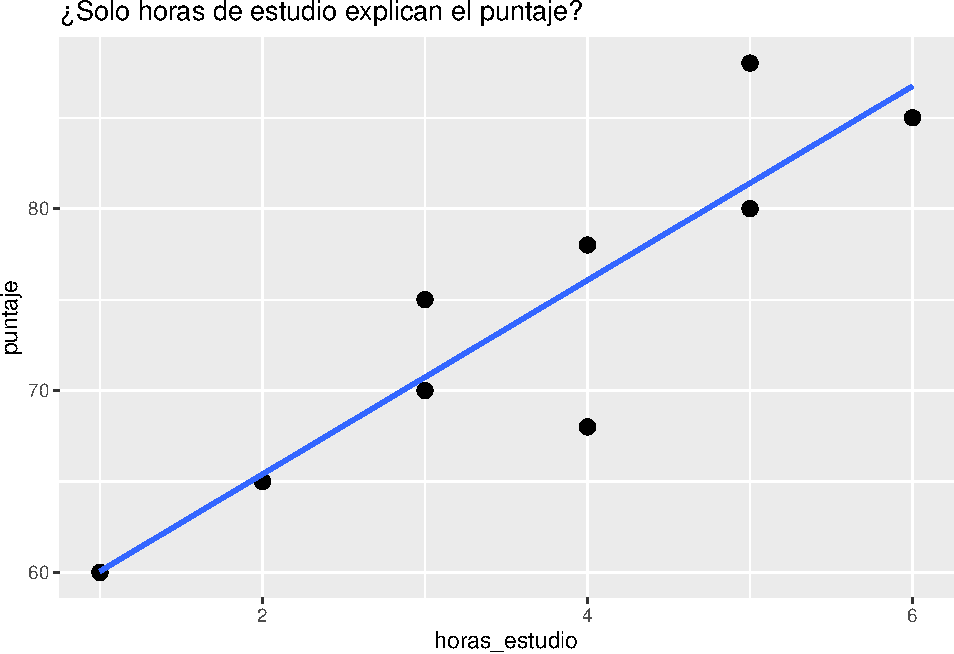
\includegraphics[keepaspectratio]{MultivariateStatisticalAnalysis_files/figure-latex/unnamed-chunk-3-1.pdf}}

¿Se ajusta un modelo lineal? ¿Porqué?

\subsection{¿Qué es ``multivariado'' y por qué lo necesitamos?}\label{quuxe9-es-multivariado-y-por-quuxe9-lo-necesitamos}

\textbf{Idea central:} cuando \textbf{varias} \(x\) influyen sobre \(y\), estudiar cada \(x\) por separado puede engañarnos. El análisis multivariado permite:

\begin{itemize}
\tightlist
\item
  \textbf{Aislar efectos}: estimar el efecto de \(x_1\) \emph{manteniendo constantes} \(x_2,x_3,...\).
\item
  \textbf{Mejorar predicción}: reducir error al añadir información relevante.
\item
  \textbf{Controlar confusores}: variables que cambian la relación aparente entre \(y\) y \(x\).
\end{itemize}

\textbf{Ejemplo:} Si ajustamos ahora un modelo con varias variables, ¿vamos a observar un cambio? ¿se ajustará mejor?

Código (modelos + comparaciones)

\begin{Shaded}
\begin{Highlighting}[]
\CommentTok{\# Modelo simple}
\NormalTok{m1 }\OtherTok{\textless{}{-}} \FunctionTok{lm}\NormalTok{(puntaje }\SpecialCharTok{\textasciitilde{}}\NormalTok{ horas\_estudio, }\AttributeTok{data =}\NormalTok{ data\_intro)}

\CommentTok{\# Modelo múltiple}
\NormalTok{m2 }\OtherTok{\textless{}{-}} \FunctionTok{lm}\NormalTok{(puntaje }\SpecialCharTok{\textasciitilde{}}\NormalTok{ horas\_estudio }\SpecialCharTok{+}\NormalTok{ horas\_sueno }\SpecialCharTok{+}\NormalTok{ asistencia, }\AttributeTok{data =}\NormalTok{ data\_intro)}

\CommentTok{\# Medidas clave}
\NormalTok{R2\_m1  }\OtherTok{\textless{}{-}} \FunctionTok{glance}\NormalTok{(m1)}\SpecialCharTok{$}\NormalTok{r.squared}
\NormalTok{R2\_m2  }\OtherTok{\textless{}{-}} \FunctionTok{glance}\NormalTok{(m2)}\SpecialCharTok{$}\NormalTok{r.squared}

\FunctionTok{print}\NormalTok{(}\FunctionTok{paste}\NormalTok{(}\StringTok{"El R2 del modelo simple:"}\NormalTok{, R2\_m1))}
\end{Highlighting}
\end{Shaded}

\begin{verbatim}
## [1] "El R2 del modelo simple: 0.824317362184441"
\end{verbatim}

\begin{Shaded}
\begin{Highlighting}[]
\FunctionTok{print}\NormalTok{(}\FunctionTok{paste}\NormalTok{(}\StringTok{"El R2 del modelo multiple:"}\NormalTok{, R2\_m2))}
\end{Highlighting}
\end{Shaded}

\begin{verbatim}
## [1] "El R2 del modelo multiple: 0.895428180549875"
\end{verbatim}

\begin{Shaded}
\begin{Highlighting}[]
\CommentTok{\#R2adj\_m1 \textless{}{-} glance(m1)$adj.r.squared}
\CommentTok{\#R2adj \_m2 \textless{}{-} glance(m2)$adj.r.squared}
\end{Highlighting}
\end{Shaded}

\begin{itemize}
\tightlist
\item
  ¿Aumentó \(R^2\) al incluir más variables? ¿Por qué tiende a subir?
\item
  ¿Qué cambia en la interpretación de horas\_estudio al controlar por horas\_sueno y asistencia?
\item
  ¿Puede un predictor ser importante en bivariado y no en multivariado (o viceversa)?
\end{itemize}

\section{Regresión múltiple}\label{regresiuxf3n-muxfaltiple-1}

\subsection{Modelo y estimación}\label{modelo-y-estimaciuxf3n}

Los modelos en regresión lineal múltiple están dados por la siguiente forma, donde \(y\) depende de \(p\) variables predictoras:

\[y_i=\beta_0+\beta_1x_{i1}+\beta_2x_{i2} + \beta_px_{ip}+\epsilon_i.\]

Se suele asumir que los errores \(\epsilon_i\) son i.i.d. con distribución normal de media 0 y varianza \(\sigma^2\) desconocida. Los coeficientes \(\beta_i\) son constantes desconocidas y son los parámetros del modelo. Cada \(\beta_j\) representa el cambio esperado en la respuesta \(y\) por el cambio unitario en \(x_i\) cuando todas las demás variables independientes \(x_i(i\neq j)\) se mantienen constantes.

\begin{Shaded}
\begin{Highlighting}[]
\CommentTok{\# Forma general}
\NormalTok{ajuste }\OtherTok{\textless{}{-}} \FunctionTok{lm}\NormalTok{(y }\SpecialCharTok{\textasciitilde{}}\NormalTok{ x1 }\SpecialCharTok{+}\NormalTok{ x2 }\SpecialCharTok{+}\NormalTok{ ... }\SpecialCharTok{+}\NormalTok{ xp, }\AttributeTok{data =}\NormalTok{ datos)}
\CommentTok{\# summary(ajuste)}
\end{Highlighting}
\end{Shaded}

Los coeficientes los podemos interpretar como sigue:

\begin{itemize}
\tightlist
\item
  \textbf{Intercepto (\(\beta_0\))}: valor esperado de \(y\) cuando todas las \(x\)=0.
\item
  \textbf{Pendiente \(\beta_j\)}: efecto \textbf{parcial} de \(x_j\) sobre \(y\) manteniendo las demás constantes.
\end{itemize}

En los modelos de regreción lineal, solemos usar las siguientes medidas de bondad de ajuste:

\begin{itemize}
\tightlist
\item
  \textbf{\(R^2\)}: proporción de varianza de \(y\) explicada.
\item
  \textbf{\(R^2\) ajustado}: penaliza por número de predictores (mejor para comparar modelos con distinto número de x).
\item
  \textbf{RMSE (\(\sigma\))}: error típico de predicción en unidades de \(y\).
\end{itemize}

\begin{Shaded}
\begin{Highlighting}[]
\NormalTok{comp }\OtherTok{\textless{}{-}}\NormalTok{ dplyr}\SpecialCharTok{::}\FunctionTok{bind\_rows}\NormalTok{(}
  \FunctionTok{glance}\NormalTok{(m1) }\SpecialCharTok{\%\textgreater{}\%} \FunctionTok{mutate}\NormalTok{(}\AttributeTok{modelo=}\StringTok{"simple"}\NormalTok{),}
  \FunctionTok{glance}\NormalTok{(m2) }\SpecialCharTok{\%\textgreater{}\%} \FunctionTok{mutate}\NormalTok{(}\AttributeTok{modelo=}\StringTok{"multiple"}\NormalTok{)}
\NormalTok{) }\SpecialCharTok{\%\textgreater{}\%} \FunctionTok{select}\NormalTok{(modelo, r.squared, adj.r.squared)}
\NormalTok{comp}
\end{Highlighting}
\end{Shaded}

\begin{verbatim}
## # A tibble: 2 x 3
##   modelo   r.squared adj.r.squared
##   <chr>        <dbl>         <dbl>
## 1 simple       0.824         0.802
## 2 multiple     0.895         0.843
\end{verbatim}

Para este modelo algunos de los supuestos se siguen del modelo de regresión lineal
simple y se agregan algunos que tienen que ver con la relación que pudiera existir entre
las variables regresoras.

\begin{itemize}
\tightlist
\item
  El modelo es lineal en los parámetros.\\
  \emph{Chequeo}: residuales vs ajustados sin patrón claro.
\item
  El modelo está especificado correctamente.
\item
  Covarianza cero entre variables regresoras y el error.
\item
  Esperanza del error igual a cero.
\item
  Homocedasticidad.
\item
  No autocorrelación entre los errores.
\item
  Los errores siguen una distribución normal.
\item
  Mas observaciones que parámetros a estimar.
\item
  Variación entre los valores de las variables regresoras.
\item
  No colinealidad (multicolinealidad) entre las variables regresoras, es decir, no existe
  una relación lineal entre \(x_i\) y \(x_j\) (es decir, las variables son linealmente independientes).
\end{itemize}

Supuestos

\begin{Shaded}
\begin{Highlighting}[]
\CommentTok{\# Modelo m2}
\FunctionTok{par}\NormalTok{(}\AttributeTok{mfrow=}\FunctionTok{c}\NormalTok{(}\DecValTok{1}\NormalTok{,}\DecValTok{2}\NormalTok{))}
\FunctionTok{plot}\NormalTok{(m2, }\AttributeTok{which=}\DecValTok{1}\NormalTok{)  }\CommentTok{\# Residuales vs ajustados}
\FunctionTok{plot}\NormalTok{(m2, }\AttributeTok{which=}\DecValTok{2}\NormalTok{)  }\CommentTok{\# QQ{-}plot}
\end{Highlighting}
\end{Shaded}

\pandocbounded{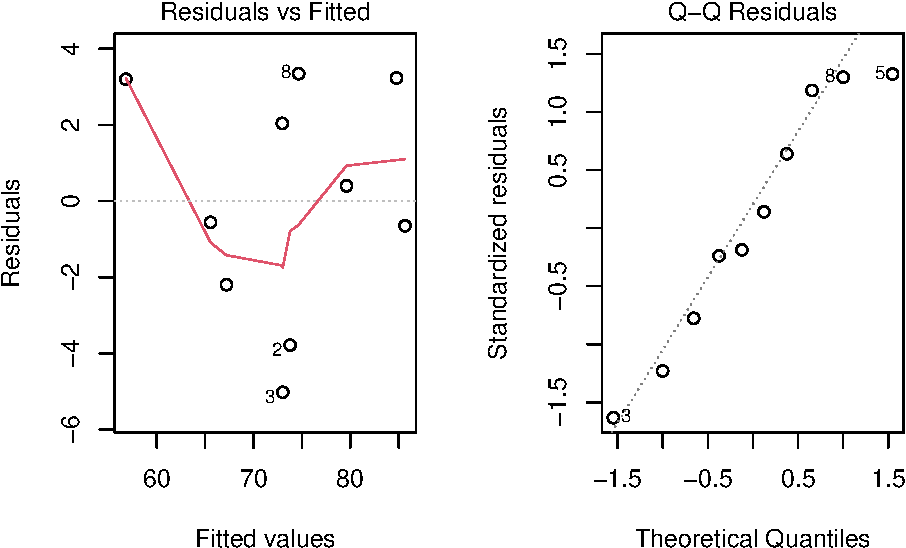
\includegraphics[keepaspectratio]{MultivariateStatisticalAnalysis_files/figure-latex/unnamed-chunk-7-1.pdf}}

\begin{center}\rule{0.5\linewidth}{0.5pt}\end{center}

\textbf{Ejercicio}: Supongamos que tenemos los siguientes datos: precio de vivienda según metros, habitaciones y distancia al centro.

Dataset

\begin{Shaded}
\begin{Highlighting}[]
\FunctionTok{set.seed}\NormalTok{(}\DecValTok{42}\NormalTok{)}
\NormalTok{n }\OtherTok{\textless{}{-}} \DecValTok{14}
\NormalTok{casas }\OtherTok{\textless{}{-}}\NormalTok{ tibble}\SpecialCharTok{::}\FunctionTok{tibble}\NormalTok{(}
  \AttributeTok{precio =} \FunctionTok{c}\NormalTok{(}\DecValTok{200}\NormalTok{,}\DecValTok{220}\NormalTok{,}\DecValTok{250}\NormalTok{,}\DecValTok{275}\NormalTok{,}\DecValTok{300}\NormalTok{,}\DecValTok{180}\NormalTok{,}\DecValTok{210}\NormalTok{,}\DecValTok{260}\NormalTok{,}\DecValTok{280}\NormalTok{,}\DecValTok{320}\NormalTok{,}\DecValTok{190}\NormalTok{,}\DecValTok{240}\NormalTok{,}\DecValTok{230}\NormalTok{,}\DecValTok{305}\NormalTok{),}
  \AttributeTok{metros =} \FunctionTok{c}\NormalTok{(}\DecValTok{80}\NormalTok{,}\DecValTok{90}\NormalTok{,}\DecValTok{100}\NormalTok{,}\DecValTok{110}\NormalTok{,}\DecValTok{120}\NormalTok{,}\DecValTok{70}\NormalTok{,}\DecValTok{85}\NormalTok{,}\DecValTok{105}\NormalTok{,}\DecValTok{115}\NormalTok{,}\DecValTok{130}\NormalTok{,}\DecValTok{75}\NormalTok{,}\DecValTok{95}\NormalTok{,}\DecValTok{92}\NormalTok{,}\DecValTok{125}\NormalTok{),}
  \AttributeTok{habitaciones =} \FunctionTok{c}\NormalTok{(}\DecValTok{2}\NormalTok{,}\DecValTok{3}\NormalTok{,}\DecValTok{3}\NormalTok{,}\DecValTok{4}\NormalTok{,}\DecValTok{4}\NormalTok{,}\DecValTok{2}\NormalTok{,}\DecValTok{3}\NormalTok{,}\DecValTok{3}\NormalTok{,}\DecValTok{4}\NormalTok{,}\DecValTok{5}\NormalTok{,}\DecValTok{2}\NormalTok{,}\DecValTok{3}\NormalTok{,}\DecValTok{3}\NormalTok{,}\DecValTok{4}\NormalTok{),}
  \AttributeTok{distancia\_centro =} \FunctionTok{c}\NormalTok{(}\DecValTok{5}\NormalTok{,}\DecValTok{4}\NormalTok{,}\DecValTok{6}\NormalTok{,}\DecValTok{3}\NormalTok{,}\DecValTok{2}\NormalTok{,}\DecValTok{8}\NormalTok{,}\DecValTok{6}\NormalTok{,}\DecValTok{3}\NormalTok{,}\DecValTok{2}\NormalTok{,}\DecValTok{1}\NormalTok{,}\DecValTok{7}\NormalTok{,}\DecValTok{5}\NormalTok{,}\DecValTok{4}\NormalTok{,}\DecValTok{2}\NormalTok{)}
\NormalTok{)}
\NormalTok{casas}
\end{Highlighting}
\end{Shaded}

\begin{verbatim}
## # A tibble: 14 x 4
##    precio metros habitaciones distancia_centro
##     <dbl>  <dbl>        <dbl>            <dbl>
##  1    200     80            2                5
##  2    220     90            3                4
##  3    250    100            3                6
##  4    275    110            4                3
##  5    300    120            4                2
##  6    180     70            2                8
##  7    210     85            3                6
##  8    260    105            3                3
##  9    280    115            4                2
## 10    320    130            5                1
## 11    190     75            2                7
## 12    240     95            3                5
## 13    230     92            3                4
## 14    305    125            4                2
\end{verbatim}

\begin{enumerate}
\def\labelenumi{\arabic{enumi})}
\tightlist
\item
  Ajusta \texttt{precio\ \textasciitilde{}\ metros} (simple) y \texttt{precio\ \textasciitilde{}\ metros\ +\ habitaciones\ +\ distancia\_centro} (múltiple).\\
\item
  Compara \(R^2\), \(R^2\) \textbf{ajustado} y \textbf{σ (RMSE)}.\\
\item
  Interpreta el coeficiente de \texttt{distancia\_centro}.\\
\item
  Revisa QQ-plot y residuales vs ajustados. ¿Algún patrón?
\end{enumerate}

Solución

\begin{Shaded}
\begin{Highlighting}[]
\NormalTok{m\_s }\OtherTok{\textless{}{-}} \FunctionTok{lm}\NormalTok{(precio }\SpecialCharTok{\textasciitilde{}}\NormalTok{ metros, }\AttributeTok{data=}\NormalTok{casas)}
\NormalTok{m\_m }\OtherTok{\textless{}{-}} \FunctionTok{lm}\NormalTok{(precio }\SpecialCharTok{\textasciitilde{}}\NormalTok{ metros }\SpecialCharTok{+}\NormalTok{ habitaciones }\SpecialCharTok{+}\NormalTok{ distancia\_centro, }\AttributeTok{data=}\NormalTok{casas)}

\NormalTok{broom}\SpecialCharTok{::}\FunctionTok{glance}\NormalTok{(m\_s)[,}\FunctionTok{c}\NormalTok{(}\StringTok{"r.squared"}\NormalTok{,}\StringTok{"adj.r.squared"}\NormalTok{)]}
\end{Highlighting}
\end{Shaded}

\begin{verbatim}
## # A tibble: 1 x 2
##   r.squared adj.r.squared
##       <dbl>         <dbl>
## 1     0.996         0.996
\end{verbatim}

\begin{Shaded}
\begin{Highlighting}[]
\NormalTok{broom}\SpecialCharTok{::}\FunctionTok{glance}\NormalTok{(m\_m)[,}\FunctionTok{c}\NormalTok{(}\StringTok{"r.squared"}\NormalTok{,}\StringTok{"adj.r.squared"}\NormalTok{)]}
\end{Highlighting}
\end{Shaded}

\begin{verbatim}
## # A tibble: 1 x 2
##   r.squared adj.r.squared
##       <dbl>         <dbl>
## 1     0.997         0.996
\end{verbatim}

\begin{Shaded}
\begin{Highlighting}[]
\NormalTok{broom}\SpecialCharTok{::}\FunctionTok{tidy}\NormalTok{(m\_m)}
\end{Highlighting}
\end{Shaded}

\begin{verbatim}
## # A tibble: 4 x 5
##   term             estimate std.error statistic      p.value
##   <chr>               <dbl>     <dbl>     <dbl>        <dbl>
## 1 (Intercept)        -8.67     14.9      -0.583 0.573       
## 2 metros              2.53      0.162    15.6   0.0000000236
## 3 habitaciones       -0.505     2.80     -0.180 0.861       
## 4 distancia_centro    1.38      0.974     1.42  0.187
\end{verbatim}

\begin{Shaded}
\begin{Highlighting}[]
\FunctionTok{par}\NormalTok{(}\AttributeTok{mfrow=}\FunctionTok{c}\NormalTok{(}\DecValTok{1}\NormalTok{,}\DecValTok{2}\NormalTok{))}
\FunctionTok{plot}\NormalTok{(m\_m, }\AttributeTok{which=}\DecValTok{1}\NormalTok{)}
\FunctionTok{plot}\NormalTok{(m\_m, }\AttributeTok{which=}\DecValTok{2}\NormalTok{)}
\end{Highlighting}
\end{Shaded}

\pandocbounded{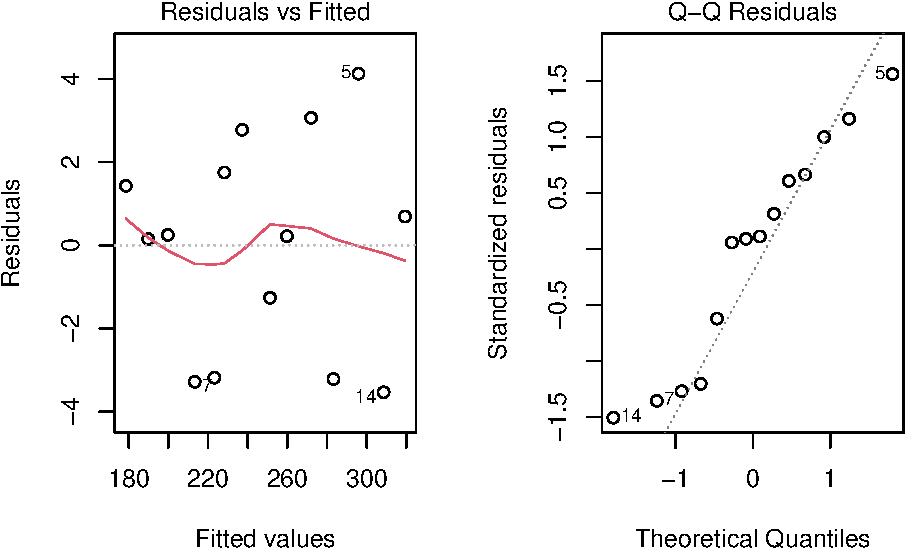
\includegraphics[keepaspectratio]{MultivariateStatisticalAnalysis_files/figure-latex/unnamed-chunk-9-1.pdf}}

\section{Estimación de parámetros}\label{estimaciuxf3n-de-paruxe1metros}

\textbf{Ejemplo (Montgomery, 2002):} : Un embotellador de bebidas gaseosas analiza las rutas de servicio de las máquinas expendedoras en su sistema de distribución. Le interesa predecir el tiempo necesario para que el representante de ruta atienda las máquinas expendedoras en una tienda.

Esta actividad de servicio consiste en abastecer la máquina con productos embotellados, y algo de mantenimiento o limpieza. El ingeniero industrial responsable del estudio ha sugerido que las dos variables más importantes que afectan el tiempo de entrega \(y\) son la cantidad de cajas de producto abastecido, \(x_1\), y la distancia caminada por el representante, \(x_2\).

El ingeniero ha reunido 25 observaciones de tiempo de entrega que se ven en la tabla siguiente. Se ajustará el modelo de regresión lineal multiple siguiente:

\[
y = \beta_0 + \beta_1 x_1 + \beta_2 x_2 +  \varepsilon
\]

\emph{Archivo: \texttt{refrescos.csv}}.

Base de datos

\begin{Shaded}
\begin{Highlighting}[]
\CommentTok{\# }
\NormalTok{datos }\OtherTok{\textless{}{-}} \FunctionTok{data.frame}\NormalTok{(}
  \AttributeTok{Observacion =} \DecValTok{1}\SpecialCharTok{:}\DecValTok{25}\NormalTok{,}
  \AttributeTok{y =} \FunctionTok{c}\NormalTok{(}\FloatTok{16.68}\NormalTok{, }\FloatTok{11.50}\NormalTok{, }\FloatTok{12.03}\NormalTok{, }\FloatTok{14.88}\NormalTok{, }\FloatTok{13.75}\NormalTok{,}
        \FloatTok{18.11}\NormalTok{, }\FloatTok{8.00}\NormalTok{, }\FloatTok{17.83}\NormalTok{, }\FloatTok{79.24}\NormalTok{, }\FloatTok{21.50}\NormalTok{,}
        \FloatTok{40.33}\NormalTok{, }\FloatTok{21.00}\NormalTok{, }\FloatTok{13.50}\NormalTok{, }\FloatTok{19.75}\NormalTok{, }\FloatTok{24.00}\NormalTok{,}
        \FloatTok{29.00}\NormalTok{, }\FloatTok{15.35}\NormalTok{, }\FloatTok{19.00}\NormalTok{, }\FloatTok{9.50}\NormalTok{, }\FloatTok{35.10}\NormalTok{,}
        \FloatTok{17.90}\NormalTok{, }\FloatTok{52.32}\NormalTok{, }\FloatTok{18.75}\NormalTok{, }\FloatTok{19.83}\NormalTok{, }\FloatTok{10.75}\NormalTok{),}
  \AttributeTok{x1 =} \FunctionTok{c}\NormalTok{(}\DecValTok{7}\NormalTok{, }\DecValTok{3}\NormalTok{, }\DecValTok{3}\NormalTok{, }\DecValTok{4}\NormalTok{, }\DecValTok{6}\NormalTok{,}
         \DecValTok{7}\NormalTok{, }\DecValTok{2}\NormalTok{, }\DecValTok{7}\NormalTok{, }\DecValTok{30}\NormalTok{, }\DecValTok{5}\NormalTok{,}
         \DecValTok{16}\NormalTok{, }\DecValTok{10}\NormalTok{, }\DecValTok{4}\NormalTok{, }\DecValTok{6}\NormalTok{, }\DecValTok{9}\NormalTok{,}
         \DecValTok{10}\NormalTok{, }\DecValTok{6}\NormalTok{, }\DecValTok{7}\NormalTok{, }\DecValTok{3}\NormalTok{, }\DecValTok{17}\NormalTok{,}
         \DecValTok{10}\NormalTok{, }\DecValTok{26}\NormalTok{, }\DecValTok{9}\NormalTok{, }\DecValTok{8}\NormalTok{, }\DecValTok{4}\NormalTok{),}
  \AttributeTok{x2 =} \FunctionTok{c}\NormalTok{(}\DecValTok{560}\NormalTok{, }\DecValTok{220}\NormalTok{, }\DecValTok{340}\NormalTok{, }\DecValTok{80}\NormalTok{, }\DecValTok{150}\NormalTok{,}
         \DecValTok{330}\NormalTok{, }\DecValTok{110}\NormalTok{, }\DecValTok{210}\NormalTok{, }\DecValTok{1460}\NormalTok{, }\DecValTok{605}\NormalTok{,}
         \DecValTok{688}\NormalTok{, }\DecValTok{215}\NormalTok{, }\DecValTok{255}\NormalTok{, }\DecValTok{462}\NormalTok{, }\DecValTok{448}\NormalTok{,}
         \DecValTok{776}\NormalTok{, }\DecValTok{200}\NormalTok{, }\DecValTok{132}\NormalTok{, }\DecValTok{36}\NormalTok{, }\DecValTok{770}\NormalTok{,}
         \DecValTok{140}\NormalTok{, }\DecValTok{810}\NormalTok{, }\DecValTok{450}\NormalTok{, }\DecValTok{635}\NormalTok{, }\DecValTok{150}\NormalTok{)}
\NormalTok{)}

\NormalTok{datos}
\end{Highlighting}
\end{Shaded}

\begin{verbatim}
##    Observacion     y x1   x2
## 1            1 16.68  7  560
## 2            2 11.50  3  220
## 3            3 12.03  3  340
## 4            4 14.88  4   80
## 5            5 13.75  6  150
## 6            6 18.11  7  330
## 7            7  8.00  2  110
## 8            8 17.83  7  210
## 9            9 79.24 30 1460
## 10          10 21.50  5  605
## 11          11 40.33 16  688
## 12          12 21.00 10  215
## 13          13 13.50  4  255
## 14          14 19.75  6  462
## 15          15 24.00  9  448
## 16          16 29.00 10  776
## 17          17 15.35  6  200
## 18          18 19.00  7  132
## 19          19  9.50  3   36
## 20          20 35.10 17  770
## 21          21 17.90 10  140
## 22          22 52.32 26  810
## 23          23 18.75  9  450
## 24          24 19.83  8  635
## 25          25 10.75  4  150
\end{verbatim}

Veamos un gráfico de dispersión de los datos. ¿Qué observamos?

\begin{Shaded}
\begin{Highlighting}[]
\FunctionTok{pairs}\NormalTok{(datos[}\SpecialCharTok{{-}}\DecValTok{1}\NormalTok{])}
\end{Highlighting}
\end{Shaded}

\pandocbounded{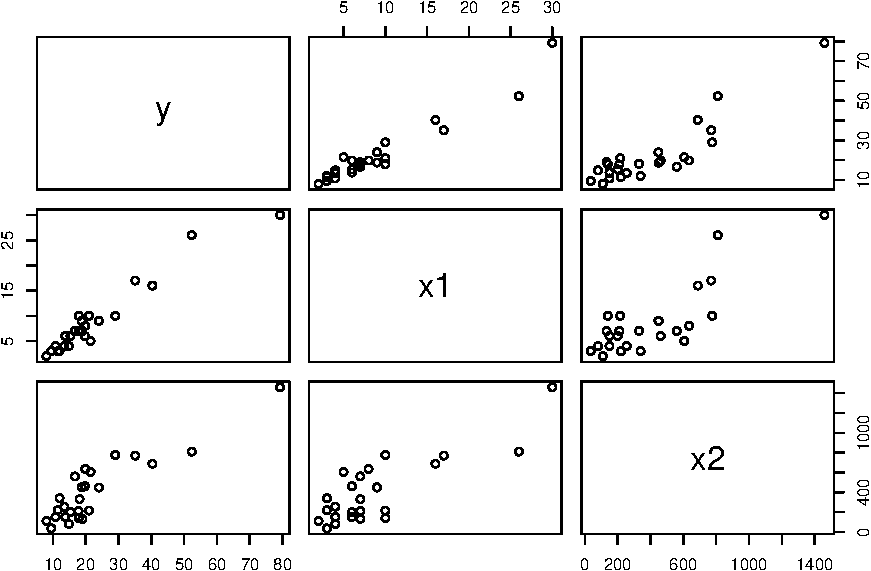
\includegraphics[keepaspectratio]{MultivariateStatisticalAnalysis_files/figure-latex/unnamed-chunk-11-1.pdf}}

\begin{enumerate}
\def\labelenumi{\arabic{enumi})}
\tightlist
\item
  Estimar \(\beta\)
\end{enumerate}

Primero, vamos a crear la matriz \(X\) y el vector \(y\).

Matrices

\begin{Shaded}
\begin{Highlighting}[]
\CommentTok{\# Columna de 1 para el intercepto}
\NormalTok{idv }\OtherTok{\textless{}{-}} \FunctionTok{rep}\NormalTok{(}\DecValTok{1}\NormalTok{, }\FunctionTok{nrow}\NormalTok{(datos))}
\CommentTok{\# Creamos matriz X}
\NormalTok{X }\OtherTok{\textless{}{-}} \FunctionTok{matrix}\NormalTok{(}\FunctionTok{c}\NormalTok{(idv,datos}\SpecialCharTok{$}\NormalTok{x1,datos}\SpecialCharTok{$}\NormalTok{x2),}\AttributeTok{nrow=}\DecValTok{25}\NormalTok{,}\AttributeTok{ncol=}\DecValTok{3}\NormalTok{)}
\CommentTok{\# Creamos el vector y}
\NormalTok{y }\OtherTok{\textless{}{-}} \FunctionTok{matrix}\NormalTok{(datos}\SpecialCharTok{$}\NormalTok{y, }\AttributeTok{nrow =} \DecValTok{25}\NormalTok{, }\AttributeTok{ncol =} \DecValTok{1}\NormalTok{)}
\end{Highlighting}
\end{Shaded}

Ya sabemos que nuestro estimador está dado por

\[
\hat{\beta} = (X'X)^{-1}X'y
\]

Entonces podemos encontrar el estimador.

Estimador beta

\begin{Shaded}
\begin{Highlighting}[]
\NormalTok{beta }\OtherTok{\textless{}{-}} \FunctionTok{solve}\NormalTok{(}\FunctionTok{t}\NormalTok{(X) }\SpecialCharTok{\%*\%}\NormalTok{ X) }\SpecialCharTok{\%*\%} \FunctionTok{t}\NormalTok{(X) }\SpecialCharTok{\%*\%}\NormalTok{ y}
\NormalTok{beta}
\end{Highlighting}
\end{Shaded}

\begin{verbatim}
##            [,1]
## [1,] 2.34123115
## [2,] 1.61590721
## [3,] 0.01438483
\end{verbatim}

Entonces el ajuste por el método de mínimos cuadrados, con los coeficientes de regresión que encontramos está dado por:

\(\hat{y} =\) 2.3412311 \(+\) 1.6159072 \(x_1\) \(+\) 1.6159072 \(x_2\)

Esto lo podemos hacer más rápido usando la función de \texttt{lm}. Construimos el modelo.

Modelo en R

\begin{Shaded}
\begin{Highlighting}[]
\NormalTok{M1 }\OtherTok{\textless{}{-}} \FunctionTok{lm}\NormalTok{(y }\SpecialCharTok{\textasciitilde{}}\NormalTok{ x1 }\SpecialCharTok{+}\NormalTok{ x2, datos)}
\NormalTok{M1 }
\end{Highlighting}
\end{Shaded}

\begin{verbatim}
## 
## Call:
## lm(formula = y ~ x1 + x2, data = datos)
## 
## Coefficients:
## (Intercept)           x1           x2  
##     2.34123      1.61591      0.01438
\end{verbatim}

¿Cómo accedemos a los valores del modelo?

Coeficientes

\begin{Shaded}
\begin{Highlighting}[]
\NormalTok{beta\_0 }\OtherTok{\textless{}{-}}\NormalTok{ M1}\SpecialCharTok{$}\NormalTok{coefficients[}\DecValTok{1}\NormalTok{]}
\NormalTok{beta\_1 }\OtherTok{\textless{}{-}}\NormalTok{ M1}\SpecialCharTok{$}\NormalTok{coefficients[}\DecValTok{2}\NormalTok{]}
\NormalTok{beta\_2 }\OtherTok{\textless{}{-}}\NormalTok{ M1}\SpecialCharTok{$}\NormalTok{coefficients[}\DecValTok{3}\NormalTok{]}
\end{Highlighting}
\end{Shaded}

Los valores son \(\beta_0=\) 2.3412311, \(\beta_1=\) 1.6159072 y \(\beta_2=\) 0.0143848.

\begin{enumerate}
\def\labelenumi{\arabic{enumi})}
\setcounter{enumi}{1}
\tightlist
\item
  Estimación de la varianza del error \(\sigma^2\)
\end{enumerate}

Ya tenemos que la suma de los cuadrados de los errores está dada por

\[ SSE = y'y - \hat{\beta}X'y\]

Sustituimos los valores que tenemos y obtemos el SSE.

SSE

\begin{Shaded}
\begin{Highlighting}[]
\NormalTok{SSE }\OtherTok{\textless{}{-}} \FunctionTok{t}\NormalTok{(y)}\SpecialCharTok{\%*\%}\NormalTok{ y }\SpecialCharTok{{-}} \FunctionTok{t}\NormalTok{(beta) }\SpecialCharTok{\%*\%} \FunctionTok{t}\NormalTok{(X) }\SpecialCharTok{\%*\%}\NormalTok{ y}
\NormalTok{SSE}
\end{Highlighting}
\end{Shaded}

\begin{verbatim}
##          [,1]
## [1,] 233.7317
\end{verbatim}

Y de está forma, podemos encontrar el estimador de \(\sigma^2\).

Estimador

\begin{Shaded}
\begin{Highlighting}[]
\NormalTok{varest }\OtherTok{\textless{}{-}}\NormalTok{ SSE }\SpecialCharTok{/}\NormalTok{ (}\FunctionTok{nrow}\NormalTok{(y) }\SpecialCharTok{{-}} \FunctionTok{nrow}\NormalTok{(beta))}
\NormalTok{varest}
\end{Highlighting}
\end{Shaded}

\begin{verbatim}
##          [,1]
## [1,] 10.62417
\end{verbatim}

Directo con las funciones de R, podemos acceder a los parámetros que se guardaron en el modelo que ya calculamos.

Resumen del modelo

\begin{Shaded}
\begin{Highlighting}[]
\FunctionTok{summary}\NormalTok{(M1)}
\end{Highlighting}
\end{Shaded}

\begin{verbatim}
## 
## Call:
## lm(formula = y ~ x1 + x2, data = datos)
## 
## Residuals:
##     Min      1Q  Median      3Q     Max 
## -5.7880 -0.6629  0.4364  1.1566  7.4197 
## 
## Coefficients:
##             Estimate Std. Error t value Pr(>|t|)    
## (Intercept) 2.341231   1.096730   2.135 0.044170 *  
## x1          1.615907   0.170735   9.464 3.25e-09 ***
## x2          0.014385   0.003613   3.981 0.000631 ***
## ---
## Signif. codes:  0 '***' 0.001 '**' 0.01 '*' 0.05 '.' 0.1 ' ' 1
## 
## Residual standard error: 3.259 on 22 degrees of freedom
## Multiple R-squared:  0.9596, Adjusted R-squared:  0.9559 
## F-statistic: 261.2 on 2 and 22 DF,  p-value: 4.687e-16
\end{verbatim}

Algunos de los parámetros almacenados en el modelo nos permiten obtener también el resultado previo.

Estimador

\begin{Shaded}
\begin{Highlighting}[]
\FunctionTok{sum}\NormalTok{(}\FunctionTok{residuals}\NormalTok{(M1)}\SpecialCharTok{\^{}}\DecValTok{2}\NormalTok{) }\SpecialCharTok{/} \FunctionTok{df.residual}\NormalTok{(M1)}
\end{Highlighting}
\end{Shaded}

\begin{verbatim}
## [1] 10.62417
\end{verbatim}

\subsection{Ejercicios}\label{ejercicios}

\textbf{Ejercicio 1:} Un analista hace un estudio químico y espera que el rendimiento de cierta sustancia se vea afectado por dos factores. Se realizan 17 experimentos cuyos datos se registran en el cuadro siguiente. Por experimentos similares, se sabe que los factores \(x_1\) y \(x_2\) no están relacionados; por ello, el analista decide utilizar un modelo de regresión lineal múltiple. Calcule el modelo de regresión y grafíquelo sobre las observaciones.

\emph{Archivo: est\_quimico.csv}

Datos Ejercicio 1

\begin{Shaded}
\begin{Highlighting}[]
\NormalTok{datos2 }\OtherTok{\textless{}{-}} \FunctionTok{data.frame}\NormalTok{(}
  \AttributeTok{Experimento =} \DecValTok{1}\SpecialCharTok{:}\DecValTok{17}\NormalTok{,}
  \AttributeTok{x1 =} \FunctionTok{c}\NormalTok{(}\FloatTok{41.9}\NormalTok{, }\FloatTok{43.4}\NormalTok{, }\FloatTok{43.9}\NormalTok{, }\FloatTok{44.5}\NormalTok{, }\FloatTok{47.3}\NormalTok{, }\FloatTok{47.5}\NormalTok{, }\FloatTok{47.9}\NormalTok{, }\FloatTok{50.2}\NormalTok{, }\FloatTok{52.8}\NormalTok{, }\FloatTok{53.2}\NormalTok{, }\FloatTok{56.7}\NormalTok{, }\FloatTok{57.0}\NormalTok{, }\FloatTok{63.5}\NormalTok{, }\FloatTok{64.3}\NormalTok{, }\FloatTok{71.1}\NormalTok{, }\FloatTok{77.0}\NormalTok{, }\FloatTok{77.8}\NormalTok{),}
  \AttributeTok{x2 =} \FunctionTok{c}\NormalTok{(}\FloatTok{29.1}\NormalTok{, }\FloatTok{29.3}\NormalTok{, }\FloatTok{29.5}\NormalTok{, }\FloatTok{29.7}\NormalTok{, }\FloatTok{29.9}\NormalTok{, }\FloatTok{30.3}\NormalTok{, }\FloatTok{30.5}\NormalTok{, }\FloatTok{30.7}\NormalTok{, }\FloatTok{30.8}\NormalTok{, }\FloatTok{30.9}\NormalTok{, }\FloatTok{31.5}\NormalTok{, }\FloatTok{31.7}\NormalTok{, }\FloatTok{31.9}\NormalTok{, }\FloatTok{32.0}\NormalTok{, }\FloatTok{32.1}\NormalTok{, }\FloatTok{32.5}\NormalTok{, }\FloatTok{32.9}\NormalTok{),}
  \AttributeTok{y  =} \FunctionTok{c}\NormalTok{(}\FloatTok{251.3}\NormalTok{, }\FloatTok{251.3}\NormalTok{, }\FloatTok{248.3}\NormalTok{, }\FloatTok{267.5}\NormalTok{, }\FloatTok{273.0}\NormalTok{, }\FloatTok{276.5}\NormalTok{, }\FloatTok{270.3}\NormalTok{, }\FloatTok{274.9}\NormalTok{, }\FloatTok{285.0}\NormalTok{, }\FloatTok{290.0}\NormalTok{, }\FloatTok{297.0}\NormalTok{, }\FloatTok{302.5}\NormalTok{, }\FloatTok{304.5}\NormalTok{, }\FloatTok{309.3}\NormalTok{, }\FloatTok{321.7}\NormalTok{, }\FloatTok{330.7}\NormalTok{, }\FloatTok{349.0}\NormalTok{)}
\NormalTok{)}

\NormalTok{datos2}
\end{Highlighting}
\end{Shaded}

\begin{verbatim}
##    Experimento   x1   x2     y
## 1            1 41.9 29.1 251.3
## 2            2 43.4 29.3 251.3
## 3            3 43.9 29.5 248.3
## 4            4 44.5 29.7 267.5
## 5            5 47.3 29.9 273.0
## 6            6 47.5 30.3 276.5
## 7            7 47.9 30.5 270.3
## 8            8 50.2 30.7 274.9
## 9            9 52.8 30.8 285.0
## 10          10 53.2 30.9 290.0
## 11          11 56.7 31.5 297.0
## 12          12 57.0 31.7 302.5
## 13          13 63.5 31.9 304.5
## 14          14 64.3 32.0 309.3
## 15          15 71.1 32.1 321.7
## 16          16 77.0 32.5 330.7
## 17          17 77.8 32.9 349.0
\end{verbatim}

\textbf{Ejercicio 2:} Repetir el ejemplo con los datos \texttt{datasets::trees} de R que proporciona mediciones
del diámetro, altura y volumen de madera en 31 cerezos negros talados.

\textbf{Ejercicio 3:} Subir a Github los dos ejercicios previos tanto con solución en R como en Python. Comparar las funciones. Ventajas y desventajas de ambas.

\section{Pruebas de Hipótesis}\label{pruebas-de-hipuxf3tesis}

Cuando revisamos el \texttt{summary} del modelo, nos arroja si son significativas o no y a que nivel de significancia las variables que estamos considerando. Veamos el siguiente ejemplo.

\subsection{Prueba de la significancia de la regresión}\label{prueba-de-la-significancia-de-la-regresiuxf3n}

\textbf{Ejemplo:} Con los datos del embotellador de bebidas gaseosas, se probará la significancia de la regresión.

Sumas de Cuadrados

\begin{Shaded}
\begin{Highlighting}[]
\NormalTok{SCT }\OtherTok{\textless{}{-}} \FunctionTok{t}\NormalTok{(y) }\SpecialCharTok{\%*\%}\NormalTok{ y }\SpecialCharTok{{-}}  \FunctionTok{sum}\NormalTok{(y)}\SpecialCharTok{**}\DecValTok{2} \SpecialCharTok{/} \FunctionTok{nrow}\NormalTok{(datos)}
\NormalTok{SCT}
\end{Highlighting}
\end{Shaded}

\begin{verbatim}
##          [,1]
## [1,] 5784.543
\end{verbatim}

\begin{Shaded}
\begin{Highlighting}[]
\NormalTok{SCE }\OtherTok{\textless{}{-}} \FunctionTok{t}\NormalTok{(beta) }\SpecialCharTok{\%*\%} \FunctionTok{t}\NormalTok{(X) }\SpecialCharTok{\%*\%}\NormalTok{ y }\SpecialCharTok{{-}} \FunctionTok{sum}\NormalTok{(y)}\SpecialCharTok{**}\DecValTok{2} \SpecialCharTok{/} \FunctionTok{nrow}\NormalTok{(datos)}
\NormalTok{SCE}
\end{Highlighting}
\end{Shaded}

\begin{verbatim}
##          [,1]
## [1,] 5550.811
\end{verbatim}

\begin{Shaded}
\begin{Highlighting}[]
\NormalTok{SSE }\OtherTok{\textless{}{-}}\NormalTok{ SCT }\SpecialCharTok{{-}}\NormalTok{ SCE}
\NormalTok{SSE}
\end{Highlighting}
\end{Shaded}

\begin{verbatim}
##          [,1]
## [1,] 233.7317
\end{verbatim}

Para probar

\[H_0 : \beta_1 = \beta_2=0\]

se calcula el estadístico:

Estadístico F

\begin{Shaded}
\begin{Highlighting}[]
\NormalTok{F0 }\OtherTok{\textless{}{-}}\NormalTok{ (SCE }\SpecialCharTok{/}\NormalTok{ (}\FunctionTok{ncol}\NormalTok{(X) }\SpecialCharTok{{-}} \DecValTok{1}\NormalTok{)) }\SpecialCharTok{/}\NormalTok{ (SSE }\SpecialCharTok{/}\NormalTok{ (}\FunctionTok{nrow}\NormalTok{(X) }\SpecialCharTok{{-}}\NormalTok{ (}\FunctionTok{ncol}\NormalTok{(X) }\SpecialCharTok{{-}}\DecValTok{1}\NormalTok{) }\SpecialCharTok{{-}} \DecValTok{1}\NormalTok{))}
\NormalTok{F0}
\end{Highlighting}
\end{Shaded}

\begin{verbatim}
##          [,1]
## [1,] 261.2351
\end{verbatim}

Como el valor de \(F_0\) es mayor que el valor tabulado de \(F_{\alpha;p,n-p-1}=F_{0.05;2;22}=3.44\), se rechaza \(H_0\). Lo cual implica qye el tiempo de entrega depende del volumen de entrega y/o de la distancia.

Ahora, usando los modelos que ya calculamos.

Sumas de cuadrados

\begin{Shaded}
\begin{Highlighting}[]
\NormalTok{SCT.m}\OtherTok{\textless{}{-}}\FunctionTok{sum}\NormalTok{((datos}\SpecialCharTok{$}\NormalTok{y}\SpecialCharTok{{-}}\FunctionTok{mean}\NormalTok{(datos}\SpecialCharTok{$}\NormalTok{y))}\SpecialCharTok{\^{}}\DecValTok{2}\NormalTok{)}
\NormalTok{SCT.m}
\end{Highlighting}
\end{Shaded}

\begin{verbatim}
## [1] 5784.543
\end{verbatim}

\begin{Shaded}
\begin{Highlighting}[]
\NormalTok{SCE.m }\OtherTok{\textless{}{-}}\FunctionTok{sum}\NormalTok{((M1}\SpecialCharTok{$}\NormalTok{fitted}\SpecialCharTok{{-}}\FunctionTok{mean}\NormalTok{(datos}\SpecialCharTok{$}\NormalTok{y))}\SpecialCharTok{\^{}}\DecValTok{2}\NormalTok{)}
\NormalTok{SCE.m}
\end{Highlighting}
\end{Shaded}

\begin{verbatim}
## [1] 5550.811
\end{verbatim}

\begin{Shaded}
\begin{Highlighting}[]
\NormalTok{SSE.m }\OtherTok{\textless{}{-}}\FunctionTok{sum}\NormalTok{(M1}\SpecialCharTok{$}\NormalTok{residuals}\SpecialCharTok{\^{}}\DecValTok{2}\NormalTok{)}
\NormalTok{SSE.m}
\end{Highlighting}
\end{Shaded}

\begin{verbatim}
## [1] 233.7317
\end{verbatim}

Grados de libertad

\begin{Shaded}
\begin{Highlighting}[]
\NormalTok{n}\OtherTok{\textless{}{-}}\FunctionTok{nrow}\NormalTok{(y)}
\NormalTok{n}
\end{Highlighting}
\end{Shaded}

\begin{verbatim}
## [1] 25
\end{verbatim}

\begin{Shaded}
\begin{Highlighting}[]
\NormalTok{GLT}\OtherTok{\textless{}{-}}\NormalTok{ n}\DecValTok{{-}1}
\NormalTok{GLT}
\end{Highlighting}
\end{Shaded}

\begin{verbatim}
## [1] 24
\end{verbatim}

\begin{Shaded}
\begin{Highlighting}[]
\NormalTok{GLRes}\OtherTok{\textless{}{-}} \FunctionTok{df.residual}\NormalTok{(M1)}
\NormalTok{GLRes}
\end{Highlighting}
\end{Shaded}

\begin{verbatim}
## [1] 22
\end{verbatim}

\begin{Shaded}
\begin{Highlighting}[]
\NormalTok{GLR}\OtherTok{\textless{}{-}}\NormalTok{ GLT}\SpecialCharTok{{-}}\NormalTok{GLRes}
\NormalTok{GLR}
\end{Highlighting}
\end{Shaded}

\begin{verbatim}
## [1] 2
\end{verbatim}

Cuadrados medios

\begin{Shaded}
\begin{Highlighting}[]
\NormalTok{CMR }\OtherTok{\textless{}{-}}\NormalTok{ SCE }\SpecialCharTok{/}\NormalTok{GLR}
\NormalTok{CMR}
\end{Highlighting}
\end{Shaded}

\begin{verbatim}
##          [,1]
## [1,] 2775.405
\end{verbatim}

\begin{Shaded}
\begin{Highlighting}[]
\NormalTok{CMRes }\OtherTok{\textless{}{-}}\NormalTok{ SSE }\SpecialCharTok{/}\NormalTok{ GLRes}
\NormalTok{CMRes}
\end{Highlighting}
\end{Shaded}

\begin{verbatim}
##          [,1]
## [1,] 10.62417
\end{verbatim}

Estadístico F\_0

\begin{Shaded}
\begin{Highlighting}[]
\NormalTok{F0 }\OtherTok{\textless{}{-}}\NormalTok{ CMR}\SpecialCharTok{/}\NormalTok{CMRes}
\NormalTok{F0}
\end{Highlighting}
\end{Shaded}

\begin{verbatim}
##          [,1]
## [1,] 261.2351
\end{verbatim}

p-valor

\begin{Shaded}
\begin{Highlighting}[]
\NormalTok{pv }\OtherTok{\textless{}{-}} \DecValTok{1} \SpecialCharTok{{-}} \FunctionTok{pf}\NormalTok{(F0, GLR,GLRes)}
\NormalTok{pv}
\end{Highlighting}
\end{Shaded}

\begin{verbatim}
##              [,1]
## [1,] 4.440892e-16
\end{verbatim}

Valor tabulado de F

\begin{Shaded}
\begin{Highlighting}[]
\NormalTok{alpha }\OtherTok{\textless{}{-}} \FloatTok{0.05}\NormalTok{; df1 }\OtherTok{\textless{}{-}} \DecValTok{2}\NormalTok{; df2 }\OtherTok{\textless{}{-}} \DecValTok{22}
\NormalTok{F\_crit }\OtherTok{\textless{}{-}} \FunctionTok{qf}\NormalTok{(}\DecValTok{1} \SpecialCharTok{{-}}\NormalTok{ alpha, df1, df2)}
\NormalTok{F\_crit}
\end{Highlighting}
\end{Shaded}

\begin{verbatim}
## [1] 3.443357
\end{verbatim}

\subsection{Pruebas sobre coeficientes individuales de regresión}\label{pruebas-sobre-coeficientes-individuales-de-regresiuxf3n}

\textbf{Ejemplo:} Usando los datos del embotellador de bebidas gaseosas, se desea evaluar la importancia de la variable regresora \emph{distancia} (\(x_2\)) dado que el regresor \emph{cajas} (\(x_1\)) está en el modelo.

Estadístico t\_0

\begin{Shaded}
\begin{Highlighting}[]
\NormalTok{C22 }\OtherTok{\textless{}{-}} \FunctionTok{solve}\NormalTok{(}\FunctionTok{t}\NormalTok{(X) }\SpecialCharTok{\%*\%}\NormalTok{ X)[}\DecValTok{3}\NormalTok{,}\DecValTok{3}\NormalTok{]}
\NormalTok{C22}
\end{Highlighting}
\end{Shaded}

\begin{verbatim}
## [1] 1.228745e-06
\end{verbatim}

\begin{Shaded}
\begin{Highlighting}[]
\NormalTok{t0 }\OtherTok{\textless{}{-}}\NormalTok{ beta\_2 }\SpecialCharTok{/} \FunctionTok{sqrt}\NormalTok{(varest }\SpecialCharTok{*}\NormalTok{ C22)}
\NormalTok{t0}
\end{Highlighting}
\end{Shaded}

\begin{verbatim}
##          [,1]
## [1,] 3.981313
\end{verbatim}

\begin{Shaded}
\begin{Highlighting}[]
\DocumentationTok{\#\# t tabulado con confianza 95\% y 22 grados de libertad}
\NormalTok{tt }\OtherTok{\textless{}{-}} \FunctionTok{qt}\NormalTok{(}\AttributeTok{p =} \FloatTok{0.95} \SpecialCharTok{+} \FloatTok{0.05}\SpecialCharTok{/}\DecValTok{2}\NormalTok{, }\AttributeTok{df =} \DecValTok{22}\NormalTok{, }\AttributeTok{lower.tail =} \ConstantTok{TRUE}\NormalTok{)}
\NormalTok{tt}
\end{Highlighting}
\end{Shaded}

\begin{verbatim}
## [1] 2.073873
\end{verbatim}

Usando el modelo que ya tenemos calculado \texttt{M1} podemos obtener estos mismos resultados de la siguiente forma.

Prueba sobre coeficientes

\begin{Shaded}
\begin{Highlighting}[]
\FunctionTok{summary}\NormalTok{(M1)}
\end{Highlighting}
\end{Shaded}

\begin{verbatim}
## 
## Call:
## lm(formula = y ~ x1 + x2, data = datos)
## 
## Residuals:
##     Min      1Q  Median      3Q     Max 
## -5.7880 -0.6629  0.4364  1.1566  7.4197 
## 
## Coefficients:
##             Estimate Std. Error t value Pr(>|t|)    
## (Intercept) 2.341231   1.096730   2.135 0.044170 *  
## x1          1.615907   0.170735   9.464 3.25e-09 ***
## x2          0.014385   0.003613   3.981 0.000631 ***
## ---
## Signif. codes:  0 '***' 0.001 '**' 0.01 '*' 0.05 '.' 0.1 ' ' 1
## 
## Residual standard error: 3.259 on 22 degrees of freedom
## Multiple R-squared:  0.9596, Adjusted R-squared:  0.9559 
## F-statistic: 261.2 on 2 and 22 DF,  p-value: 4.687e-16
\end{verbatim}

\section{Intervalos de confianza}\label{intervalos-de-confianza}

\subsection{Intervalos de confianza en los coeficientes de regresión}\label{intervalos-de-confianza-en-los-coeficientes-de-regresiuxf3n}

\textbf{Ejemplo:} Usando los datos del embotellador de bebidas gaseosas, queremos calcular el intervalo de confianza del 95\% para \(\beta_1\). Recordemos que el estimador puntual de \(\beta_1\) es 1.6159072.

Intervalo de confianza

\begin{Shaded}
\begin{Highlighting}[]
\NormalTok{C11 }\OtherTok{\textless{}{-}} \FunctionTok{solve}\NormalTok{(}\FunctionTok{t}\NormalTok{(X) }\SpecialCharTok{\%*\%}\NormalTok{ X)[}\DecValTok{2}\NormalTok{,}\DecValTok{2}\NormalTok{]}

\NormalTok{izq }\OtherTok{\textless{}{-}}\NormalTok{ beta\_1 }\SpecialCharTok{{-}}\NormalTok{ tt }\SpecialCharTok{*} \FunctionTok{sqrt}\NormalTok{(varest}\SpecialCharTok{*}\NormalTok{C11)}
\NormalTok{izq}
\end{Highlighting}
\end{Shaded}

\begin{verbatim}
##          [,1]
## [1,] 1.261825
\end{verbatim}

\begin{Shaded}
\begin{Highlighting}[]
\NormalTok{der }\OtherTok{\textless{}{-}}\NormalTok{ beta\_1 }\SpecialCharTok{+}\NormalTok{ tt }\SpecialCharTok{*} \FunctionTok{sqrt}\NormalTok{(varest}\SpecialCharTok{*}\NormalTok{C11)}
\NormalTok{der}
\end{Highlighting}
\end{Shaded}

\begin{verbatim}
##         [,1]
## [1,] 1.96999
\end{verbatim}

\subsection{Intervalo de confianza de la respuesta media}\label{intervalo-de-confianza-de-la-respuesta-media}

\textbf{Ejemplo:} El embotellador de bebidas gaseosas quiere establecer un intervalo de confianza del 95\% para el tiempo medio de entrega para una tienda donde se requieren \(x_1=8\) cajas y la distancia es de \(x_2=275\) pies.

Nuestro vector \(X_0\) está dado por:

X0

\begin{Shaded}
\begin{Highlighting}[]
\NormalTok{X0 }\OtherTok{\textless{}{-}} \FunctionTok{matrix}\NormalTok{(}\FunctionTok{c}\NormalTok{(}\DecValTok{1}\NormalTok{, }\DecValTok{8}\NormalTok{, }\DecValTok{275}\NormalTok{), }\AttributeTok{nrow =} \DecValTok{3}\NormalTok{)}
\NormalTok{X0}
\end{Highlighting}
\end{Shaded}

\begin{verbatim}
##      [,1]
## [1,]    1
## [2,]    8
## [3,]  275
\end{verbatim}

El valor ajustado en ese punto es:

Valor ajustado

\begin{Shaded}
\begin{Highlighting}[]
\NormalTok{y0 }\OtherTok{\textless{}{-}} \FunctionTok{t}\NormalTok{(X0) }\SpecialCharTok{\%*\%}\NormalTok{ beta}
\NormalTok{y0}
\end{Highlighting}
\end{Shaded}

\begin{verbatim}
##          [,1]
## [1,] 19.22432
\end{verbatim}

La varianza de \(\hat{y_0}\)

Varianza

\begin{Shaded}
\begin{Highlighting}[]
\NormalTok{var\_y0 }\OtherTok{\textless{}{-}}\NormalTok{ varest }\SpecialCharTok{*} \FunctionTok{t}\NormalTok{(X0) }\SpecialCharTok{\%*\%} \FunctionTok{solve}\NormalTok{(}\FunctionTok{t}\NormalTok{(X) }\SpecialCharTok{\%*\%}\NormalTok{ X) }\SpecialCharTok{\%*\%}\NormalTok{ X0}
\NormalTok{var\_y0}
\end{Highlighting}
\end{Shaded}

\begin{verbatim}
##           [,1]
## [1,] 0.5734134
\end{verbatim}

Entonces el intervalo de confianza en este punto es:

Intervalo de confianza

\begin{Shaded}
\begin{Highlighting}[]
\NormalTok{l\_izq }\OtherTok{\textless{}{-}}\NormalTok{ y0 }\SpecialCharTok{{-}}\NormalTok{ tt }\SpecialCharTok{*} \FunctionTok{sqrt}\NormalTok{(var\_y0) }
\NormalTok{l\_izq}
\end{Highlighting}
\end{Shaded}

\begin{verbatim}
##         [,1]
## [1,] 17.6539
\end{verbatim}

\begin{Shaded}
\begin{Highlighting}[]
\NormalTok{l\_der }\OtherTok{\textless{}{-}}\NormalTok{ y0 }\SpecialCharTok{+}\NormalTok{ tt }\SpecialCharTok{*} \FunctionTok{sqrt}\NormalTok{(var\_y0) }
\NormalTok{l\_der}
\end{Highlighting}
\end{Shaded}

\begin{verbatim}
##          [,1]
## [1,] 20.79474
\end{verbatim}

\textbf{Ejemplo: } Usaremos el conjunto de datos \texttt{data("marketing")} que contiene 200 observaciones de un experimento publicitario que evalúa el impacto de tres medios de anuncio en las ventas. Para cada observación se registran los presupuestos de publicidad (en miles de dólares) y las ventas obtenidas.
Variables:

\begin{itemize}
\tightlist
\item
  \texttt{youtube}: presupuesto invertido en anuncios de YouTube (miles de USD).
\item
  \texttt{facebook}: presupuesto invertido en Facebook (miles de USD).
\item
  \texttt{newspaper}: presupuesto invertido en prensa escrita (miles de USD).
\item
  \texttt{sales}: ventas registradas (variable respuesta).
\end{itemize}

Cargamos los datos:

\begin{Shaded}
\begin{Highlighting}[]
\FunctionTok{library}\NormalTok{(datarium)}
\FunctionTok{data}\NormalTok{(}\StringTok{"marketing"}\NormalTok{)}
\end{Highlighting}
\end{Shaded}

Exploramos rápidamente la base para ver qué variables contiene y la dimensión:

\begin{Shaded}
\begin{Highlighting}[]
\FunctionTok{str}\NormalTok{(marketing)}
\end{Highlighting}
\end{Shaded}

\begin{verbatim}
## 'data.frame':    200 obs. of  4 variables:
##  $ youtube  : num  276.1 53.4 20.6 181.8 217 ...
##  $ facebook : num  45.4 47.2 55.1 49.6 13 ...
##  $ newspaper: num  83 54.1 83.2 70.2 70.1 ...
##  $ sales    : num  26.5 12.5 11.2 22.2 15.5 ...
\end{verbatim}

\begin{Shaded}
\begin{Highlighting}[]
\CommentTok{\#?marketing}
\end{Highlighting}
\end{Shaded}

Ajustamos un modelo lineal que incluya todas las variables, es decir,

\(sales=\beta_0+\beta_1 youtube+\beta_2 facebook+ \beta_3 newspaper+\epsilon\)

Modelo marketing

\begin{Shaded}
\begin{Highlighting}[]
\NormalTok{modelo1}\OtherTok{\textless{}{-}}\FunctionTok{lm}\NormalTok{(sales}\SpecialCharTok{\textasciitilde{}}\NormalTok{youtube}\SpecialCharTok{+}\NormalTok{facebook}\SpecialCharTok{+}\NormalTok{newspaper,}\AttributeTok{data=}\NormalTok{marketing)}
\FunctionTok{summary}\NormalTok{(modelo1)}
\end{Highlighting}
\end{Shaded}

\begin{verbatim}
## 
## Call:
## lm(formula = sales ~ youtube + facebook + newspaper, data = marketing)
## 
## Residuals:
##      Min       1Q   Median       3Q      Max 
## -10.5932  -1.0690   0.2902   1.4272   3.3951 
## 
## Coefficients:
##              Estimate Std. Error t value Pr(>|t|)    
## (Intercept)  3.526667   0.374290   9.422   <2e-16 ***
## youtube      0.045765   0.001395  32.809   <2e-16 ***
## facebook     0.188530   0.008611  21.893   <2e-16 ***
## newspaper   -0.001037   0.005871  -0.177     0.86    
## ---
## Signif. codes:  0 '***' 0.001 '**' 0.01 '*' 0.05 '.' 0.1 ' ' 1
## 
## Residual standard error: 2.023 on 196 degrees of freedom
## Multiple R-squared:  0.8972, Adjusted R-squared:  0.8956 
## F-statistic: 570.3 on 3 and 196 DF,  p-value: < 2.2e-16
\end{verbatim}

¿Qué se puede decir sobre la significancia de la variable \(newspaper\)?

Veamos qué ocurre con el modelo al eliminar la variable \(newspaper\)

Modelo marketing 2

\begin{Shaded}
\begin{Highlighting}[]
\NormalTok{modelo2}\OtherTok{\textless{}{-}}\FunctionTok{lm}\NormalTok{(sales}\SpecialCharTok{\textasciitilde{}}\NormalTok{facebook}\SpecialCharTok{+}\NormalTok{youtube,}\AttributeTok{data=}\NormalTok{marketing)}
\FunctionTok{summary}\NormalTok{(modelo2)}
\end{Highlighting}
\end{Shaded}

\begin{verbatim}
## 
## Call:
## lm(formula = sales ~ facebook + youtube, data = marketing)
## 
## Residuals:
##      Min       1Q   Median       3Q      Max 
## -10.5572  -1.0502   0.2906   1.4049   3.3994 
## 
## Coefficients:
##             Estimate Std. Error t value Pr(>|t|)    
## (Intercept)  3.50532    0.35339   9.919   <2e-16 ***
## facebook     0.18799    0.00804  23.382   <2e-16 ***
## youtube      0.04575    0.00139  32.909   <2e-16 ***
## ---
## Signif. codes:  0 '***' 0.001 '**' 0.01 '*' 0.05 '.' 0.1 ' ' 1
## 
## Residual standard error: 2.018 on 197 degrees of freedom
## Multiple R-squared:  0.8972, Adjusted R-squared:  0.8962 
## F-statistic: 859.6 on 2 and 197 DF,  p-value: < 2.2e-16
\end{verbatim}

Lo que sigue, es hacer pruebas de hipótesis tanto en las variables como en los coeficientes de regresión.

\subsection{Ejercicios}\label{ejercicios-1}

\textbf{Ejercicio 1:} Realizar las pruebas de hipótesis sobre la significancia de la regresión y sobre los coeficientes. Encontrar los intervalos de confianza respectivos del 95\%.
Para una tienda con presupuestos:
\(youtube = 150\), \(facebook = 30\), \(newspaper=20\) (en miles de USD):
(a) Calcula el intervalo de confianza del 95\% para la media de ventas \(\mathbb{E}(sales | X_0)\).
(b) Calcula el intervalo de predicción del 95\% para una nueva observación de ventas.
(c) Comenta la diferencia entre ambos intervalos.
Subir respuesta y explicación de sus resultados a github.

\section{Ejercicios Regresión Lineal Multiple}\label{ejercicios-regresiuxf3n-lineal-multiple}

Realiza los siguientes ejercicios. En cada inciso:

\begin{itemize}
\item
  explica y comenta la solución,
\item
  incluye el código utilizado, y
\item
  añade las gráficas (plots) correspondientes con su interpretación.
\end{itemize}

Asegúrate de que el código sea reproducible y que las figuras tengan títulos, ejes y leyendas.

\textbf{Ejercicio 1:} Para los datos de la \href{https://github.com/HaydeePeruyero/MultivariateStatisticalAnalysis/tree/main/data/Liga_nacional_de_futbol.csv}{Liga Nacional de Fútbol}. Realizar tanto con las funciones de R y Python como con las fórmulas que usan matrices.

\begin{enumerate}
\def\labelenumi{\alph{enumi})}
\item
  Ajustar un modelo de regresión lineal múltiple que relacione la cantidad de juegos ganados con las yardas por aire del equipo (\(x_2\)), el porcentaje de jugadas por tierra (\(x_7\)) y las yardas por tierra del contrario (\(x_8\)).
\item
  Formar la tabla de análisis de varianza y probar la significancia de la regresión.
\item
  Calcular el estadístico \emph{t} para probar las hipótesis \(H_0 : \beta_2 = 0\), \(H_0 : \beta_7 = 0\) y \(H_0 : \beta_8 = 0\). ¿Qué conclusiones se pueden sacar acerca del papel de las variables \(x_2\), \(x_7\) y \(x_8\) en el modelo?
\item
  Calcular \(R^2\) y \(R^2_{adj}\) para este modelo.
\item
  Trazar una gráfica de probabilidad normal de los residuales. ¿Parece haber algún problema con la hipótesis de normalidad?
\item
  Trazar e interpretar una gráfica de los residuales en función de la respuesta predicha.
\item
  Trazar las gráficas de los residuales en función de cada una de las variables regresoras. ¿Implican esas gráficas que se especificó en forma correcta el regresor?
\item
  Calcular un intervalo de confianza de \(95\%\) para \(\beta_7\) y un intervalo de confianza de \(95\%\) para la cantidad media de juegos ganados por un equipo cuando \(x_2 = 2300\), \(x_7 = 56\) y \(x_8 = 2100\).
\item
  Ajustar un modelo a esos datos, usando solo \(x_7\) y \(x_8\) como regresores y probar la significancia de la regresión.
\item
  Calcular \(R^2\) y \(R^2_{adj}\). Compararlos con los resultados del modelo anterior.
\item
  Calcular un intervalo de confianza de \(95\%\) para \(\beta_7\). También, un intervalo de confianza de \(95\%\) para la cantidad media de juegos ganados por un equipo cuando \(x_7 = 56\) y \(x_8 = 2100\). Comparar las longitudes de esos intervalos de confianza con las longitudes de los correspondientes al modelo anterior.
\item
  ¿Qué conclusiones se pueden sacar de este problema, acerca de las consecuencias de omitir un regresor importante de un modelo?
\end{enumerate}

\emph{Descripción de las variables:}

\(y\): Juegos ganados (por temporada de 14 juegos)

\(x_{1}\): Yardas por tierra (temporada)

\(x_{2}\): Yardas por aire (temporada)

\(x_{3}\): Promedio de pateo (yardas/patada)

\(x_{4}\): Porcentaje de goles de campo (GC hechos/GC intentados, temporada)

\(x_{5}\): Diferencia de pérdidas de balón (pérdidas ganadas/pérdidas perdidas)

\(x_{6}\): Yardas de castigo (temporada)

\(x_{7}\): Porcentaje de carreras (jugadas por tierra/jugadas totales)

\(x_{8}\): Yardas por tierra del contrario (temporada)

\(x_{9}\): Yardas por aire del contrario (temporada)

\textbf{Ejericio 2:} Véase los datos de \href{https://github.com/HaydeePeruyero/MultivariateStatisticalAnalysis/tree/main/data/Rendimiento_de_gasolina.csv}{rendimiento de gasolina}. Realizar el ejercicio en R.

\begin{enumerate}
\def\labelenumi{\alph{enumi})}
\item
  Ajustar un modelo de regresión lineal múltiple que relacione el rendimiento de la gasolina \emph{y}, en millas por galón, la cilindrada del motor (\(x_1\)) y la cantidad de gargantas del carburador (\(x_6\)).
\item
  Formar la tabla de análisis de varianza y probar la significancia de la regresión.
\item
  Calcular \(R^2\) y \(R^2_{adj}\) para este modelo. Compararlas con las \(R^2\) y \(R^2_{adj}\) Ajustado para el modelo de regresión lineal simple, que relaciona las millas con la cilindrada.
\item
  Determinar un intervalo de confianza para \(\beta_1\).
\item
  Determinar un intervalo de confianza de \(95\%\) para el rendimiento promedio de la gasolina, cuando \(x_1 = 225 pulg^3\) y \(x_6 = 2\) gargantas.
\item
  Determinar un intervalo de predicción de \(95\%\) para una nueva observación de rendimiento de gasolina, cuando \(x_1 = 225 pulg^3\) y \(x_6 = 2\) gargantas.
\item
  Considerar el modelo de regresión lineal simple, que relaciona las millas con la cilindrada. Construir un intervalo de confianza de \(95\%\) para el rendimiento promedio de la gasolina y un intervalo de predicción para el rendimiento, cuando \(x_1 = 225 pulg^3\). Comparar las longitudes de estos intervalos con los intervalos obtenidos en los dos incisos anteriores. ¿Tiene ventajas agregar \(x_6\) al modelo?
\item
  Trazar una gráfica de probabilidad normal de los residuales. ¿Parece haber algún problema con la hipótesis de normalidad?
\item
  Trazar e interpretar una gráfica de los residuales en función de la respuesta predicha.
\item
  Trazar las gráficas de los residuales en función de cada una de las variables regresoras. ¿Implican esas gráficas que se especificó en forma correcta el regresor?
\end{enumerate}

\emph{Descripción de variables:} Variables (Fuente: Motor Trend, 1975)

\(y:\) Millas/galón

\(x_1:\) Cilindrada (pulgadas cúbicas)

\(x_2:\) Potencia (Hp)

\(x_3:\) Par de torsión (pies-lb)

\(x_4:\) Relación de compresión

\(x_5:\) Relación de eje trasero

\(x_6:\) Carburador (gargantas)

\(x_7:\) Número de velocidades en la transmisión

\(x_8:\) Longitud total (pulgadas)

\(x_9:\) Ancho (pulgadas)

\(x_{10}:\) Peso (lb)

\(x_{11}:\) Tipo de transmisión (1 = automática, 0 = manual)

\textbf{Ejercicio 3:} Véase los datos sobre \href{https://github.com/HaydeePeruyero/MultivariateStatisticalAnalysis/tree/main/data/Precios_de_viviendas}{precios de viviendas}. Realizar el ejercicio en Python.

\begin{enumerate}
\def\labelenumi{\alph{enumi})}
\item
  Ajustar un modelo de regresión lineal múltiple que relacione el precio de venta con los nueve regresores.
\item
  Probar la significancia de la regresión.¿Qué conclusiones se pueden sacar?
\item
  Usar pruebas t para evaluar la contribución de cada regresor al modelo.
\item
  Calcular \(R^2\) y \(R^2_{adj}\) para este modelo.
\item
  ¿Cuál es la contribución del tamaño del lote y el espacio vital para el modelo, dado que se incluyeron todos los demás regresores?.
\item
  En este modelo, ¿la colinealidad es un problema potencial?
\item
  Trazar una gráfica de probabilidad normal de los residuales. ¿Parece haber algún problema con la hipótesis de normalidad?
\item
  Trazar e interpretar una gráfica de los residuales en función de la respuesta predicha.
\item
  Trazar las gráficas de los residuales en función de cada una de las variables regresoras. ¿Implican esas gráficas que se especificó en forma correcta el regresor?.
\end{enumerate}

\emph{Descripción de las variables:}

\(y\): Precio de venta de la casa / 1000

\(x_{1}\): Impuestos (locales, escuela, municipal) / 1000

\(x_{2}\): Cantidad de baños

\(x_{3}\): Tamaño del terreno (pies cuadrados \(\times\) 1000)

\(x_{4}\): Superficie construida (pies cuadrados \(\times\) 1000)

\(x_{5}\): Cantidad de cajones en cochera

\(x_{6}\): Cantidad de habitaciones

\(x_{7}\): Cantidad de recámaras

\(x_{8}\): Edad de la casa (años)

\(x_{9}\): Cantidad de chimeneas

\textbf{Ejercicio 4:} Explica lo siguiente.

\begin{enumerate}
\def\labelenumi{\alph{enumi})}
\item
  ¿Qué supuestos del modelo de regresión lineal múltiple deben verificarse?
\item
  ¿Cómo se interpretan los intervalos de confianza? Si construimos un intervalo de confianza del 95\% para un coeficiente \(\beta_j\), ¿cuál sería la lectura correcta o interpretación correcta sobre este intervalo?
\item
  Describe los métodos de selección de variables y sus ventajas y desventajas:
\item
  Selección hacia adelante (forward)
\end{enumerate}

\begin{enumerate}
\def\labelenumi{\roman{enumi})}
\setcounter{enumi}{1}
\item
  Selección hacia atrás (backward)
\item
  selección por pasos (stepwise) y/o mejor subconjunto (best subset)
\end{enumerate}

Explica cómo se utilizan para elegir el modelo final.

\textbf{Ejercicio 5:} Para los datos del ejercicio 1 de la liga de Futbol. Realizar el ejercicio en R y Python.

\begin{enumerate}
\def\labelenumi{\alph{enumi})}
\item
  Usar el algoritmo de selección hacia adelante para seleccionar un modelo de regresión.
\item
  Usar el algoritmo de selección hacia atrás para seleccionar un modelo de regresión.
\item
  Usar el algoritmo de regresión por pasos para seleccionar un modelo de regresión.
\item
  Comenta los modelos finales en cada uno de los casos anteriores. ¿Cuál tiene más sentido? ¿Cuál modelo usarían?
\end{enumerate}

\section{Validación de Supuestos}\label{validaciuxf3n-de-supuestos}

\textbf{Ejemplo:} Se llevó a cabo un conjunto de ensayos experimentales con un horno para determinar una forma de predecir el tiempo de cocción, \(y\), a diferentes niveles de ancho del horno, \(x_1\), y a diferentes temperaturas, \(x_2\). Se registraron los siguientes datos:

\begin{Shaded}
\begin{Highlighting}[]
\NormalTok{yp }\OtherTok{\textless{}{-}}\FunctionTok{c}\NormalTok{(}\FloatTok{6.40}\NormalTok{, }\FloatTok{15.05}\NormalTok{, }\FloatTok{18.75}\NormalTok{, }\FloatTok{30.25}\NormalTok{, }\FloatTok{44.85}\NormalTok{, }\FloatTok{48.85}\NormalTok{, }\FloatTok{51.55}\NormalTok{, }\FloatTok{61.50}\NormalTok{, }\FloatTok{100.44}\NormalTok{, }\FloatTok{111.42}\NormalTok{)}
\NormalTok{x1 }\OtherTok{\textless{}{-}}\FunctionTok{c}\NormalTok{(}\FloatTok{1.32}\NormalTok{, }\FloatTok{2.69}\NormalTok{, }\FloatTok{3.56}\NormalTok{, }\FloatTok{4.41}\NormalTok{, }\FloatTok{5.35}\NormalTok{, }\FloatTok{6.20}\NormalTok{, }\FloatTok{7.12}\NormalTok{, }\FloatTok{8.87}\NormalTok{, }\FloatTok{9.80}\NormalTok{, }\FloatTok{10.65}\NormalTok{)}
\NormalTok{x2 }\OtherTok{\textless{}{-}}\FunctionTok{c}\NormalTok{(}\FloatTok{1.15}\NormalTok{, }\FloatTok{3.40}\NormalTok{, }\FloatTok{4.10}\NormalTok{, }\FloatTok{8.75}\NormalTok{, }\FloatTok{14.82}\NormalTok{, }\FloatTok{15.15}\NormalTok{, }\FloatTok{15.32}\NormalTok{, }\FloatTok{18.18}\NormalTok{, }\FloatTok{35.19}\NormalTok{, }\FloatTok{40.40}\NormalTok{)}
\NormalTok{datos}\OtherTok{\textless{}{-}}\FunctionTok{data.frame}\NormalTok{(yp, x1, x2)}
\FunctionTok{kable}\NormalTok{(datos, }\AttributeTok{caption =} \StringTok{"Factores que influyen en el tiempo de coccion segun diferentes niveles de ancho del horno y diferentes temperaturas"}\NormalTok{)}
\end{Highlighting}
\end{Shaded}

\begin{table}

\caption{\label{tab:unnamed-chunk-40}Factores que influyen en el tiempo de coccion segun diferentes niveles de ancho del horno y diferentes temperaturas}
\centering
\begin{tabular}[t]{r|r|r}
\hline
yp & x1 & x2\\
\hline
6.40 & 1.32 & 1.15\\
\hline
15.05 & 2.69 & 3.40\\
\hline
18.75 & 3.56 & 4.10\\
\hline
30.25 & 4.41 & 8.75\\
\hline
44.85 & 5.35 & 14.82\\
\hline
48.85 & 6.20 & 15.15\\
\hline
51.55 & 7.12 & 15.32\\
\hline
61.50 & 8.87 & 18.18\\
\hline
100.44 & 9.80 & 35.19\\
\hline
111.42 & 10.65 & 40.40\\
\hline
\end{tabular}
\end{table}

\begin{itemize}
\item
  Variable dependiente \(y =\) tiempo de cocción
\item
  Variable independiente \(x_1 =\) ancho del horno
\item
  Variable independiente \(x_2 =\) diferentes temperaturas
\end{itemize}

Vamos a visualizar los datos:

Plot

\begin{Shaded}
\begin{Highlighting}[]
\NormalTok{g1 }\OtherTok{\textless{}{-}} \FunctionTok{ggplot}\NormalTok{(}\AttributeTok{data =}\NormalTok{ datos, }\AttributeTok{mapping =} \FunctionTok{aes}\NormalTok{(}\AttributeTok{x =}\NormalTok{ x1, }\AttributeTok{y =}\NormalTok{ yp)) }\SpecialCharTok{+}
  \FunctionTok{geom\_point}\NormalTok{(}\AttributeTok{color =} \StringTok{"forestgreen"}\NormalTok{, }\AttributeTok{size =} \DecValTok{2}\NormalTok{) }\SpecialCharTok{+}
  \FunctionTok{labs}\NormalTok{(}\AttributeTok{title  =}  \StringTok{\textquotesingle{}yp \textasciitilde{} x1\textquotesingle{}}\NormalTok{, }\AttributeTok{x  =}  \StringTok{\textquotesingle{}x1\textquotesingle{}}\NormalTok{) }\SpecialCharTok{+}
  \FunctionTok{geom\_smooth}\NormalTok{(}\AttributeTok{method =} \StringTok{"lm"}\NormalTok{, }\AttributeTok{se =} \ConstantTok{FALSE}\NormalTok{, }\AttributeTok{color =} \StringTok{"black"}\NormalTok{) }\SpecialCharTok{+}
  \FunctionTok{theme\_bw}\NormalTok{() }\SpecialCharTok{+}
  \FunctionTok{theme}\NormalTok{(}\AttributeTok{plot.title =} \FunctionTok{element\_text}\NormalTok{(}\AttributeTok{hjust =} \FloatTok{0.5}\NormalTok{)) }

\NormalTok{g2 }\OtherTok{\textless{}{-}} \FunctionTok{ggplot}\NormalTok{(}\AttributeTok{data =}\NormalTok{ datos, }\AttributeTok{mapping =} \FunctionTok{aes}\NormalTok{(}\AttributeTok{x =}\NormalTok{ x2, }\AttributeTok{y =}\NormalTok{ yp)) }\SpecialCharTok{+}
  \FunctionTok{geom\_point}\NormalTok{(}\AttributeTok{color =} \StringTok{"orange"}\NormalTok{, }\AttributeTok{size =} \DecValTok{2}\NormalTok{) }\SpecialCharTok{+}
  \FunctionTok{labs}\NormalTok{(}\AttributeTok{title  =}  \StringTok{\textquotesingle{}yp \textasciitilde{} x2\textquotesingle{}}\NormalTok{, }\AttributeTok{x  =}  \StringTok{\textquotesingle{}x2\textquotesingle{}}\NormalTok{) }\SpecialCharTok{+}
  \FunctionTok{geom\_smooth}\NormalTok{(}\AttributeTok{method =} \StringTok{"lm"}\NormalTok{, }\AttributeTok{se =} \ConstantTok{FALSE}\NormalTok{, }\AttributeTok{color =} \StringTok{"black"}\NormalTok{) }\SpecialCharTok{+}
  \FunctionTok{theme\_bw}\NormalTok{() }\SpecialCharTok{+}
  \FunctionTok{theme}\NormalTok{(}\AttributeTok{plot.title =} \FunctionTok{element\_text}\NormalTok{(}\AttributeTok{hjust =} \FloatTok{0.5}\NormalTok{))}

\NormalTok{g1}\SpecialCharTok{+}\NormalTok{g2}
\end{Highlighting}
\end{Shaded}

\begin{verbatim}
## `geom_smooth()` using formula = 'y ~ x'
## `geom_smooth()` using formula = 'y ~ x'
\end{verbatim}

\pandocbounded{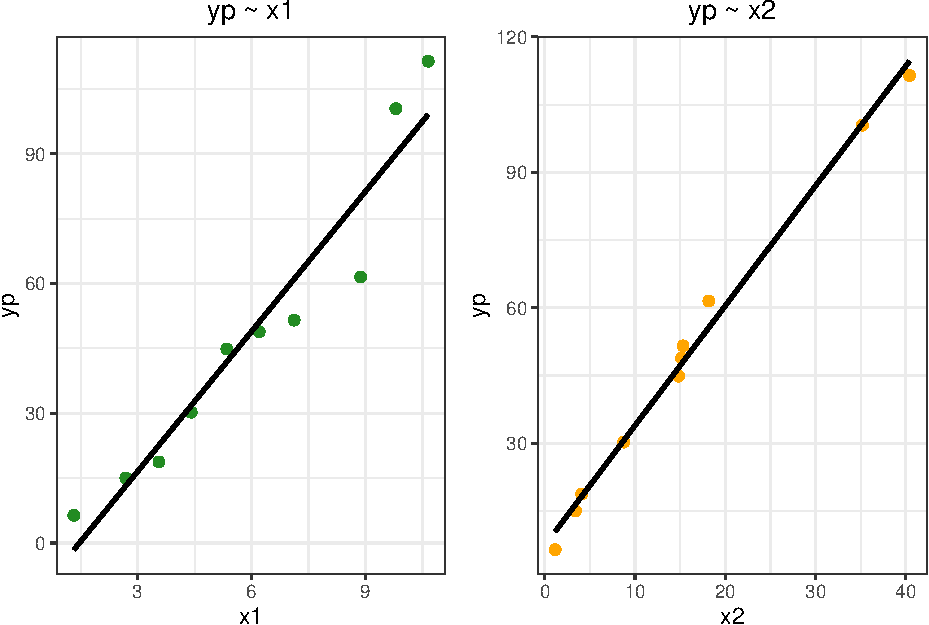
\includegraphics[keepaspectratio]{MultivariateStatisticalAnalysis_files/figure-latex/unnamed-chunk-41-1.pdf}}

Ahora, vamos a analizar algunos de los supuestos.

\subsection{Multicolinealidad}\label{multicolinealidad}

Multicolinealidad

\begin{Shaded}
\begin{Highlighting}[]
\NormalTok{variables }\OtherTok{\textless{}{-}} \FunctionTok{data.frame}\NormalTok{(x1,x2)}
\NormalTok{m\_cor }\OtherTok{\textless{}{-}} \FunctionTok{cor}\NormalTok{(variables,}\AttributeTok{method =} \StringTok{"pearson"}\NormalTok{)}
\NormalTok{m\_cor}
\end{Highlighting}
\end{Shaded}

\begin{verbatim}
##           x1        x2
## x1 1.0000000 0.9375592
## x2 0.9375592 1.0000000
\end{verbatim}

Plot

\begin{Shaded}
\begin{Highlighting}[]
\FunctionTok{library}\NormalTok{(corrplot)}
\end{Highlighting}
\end{Shaded}

\begin{verbatim}
## corrplot 0.95 loaded
\end{verbatim}

\begin{Shaded}
\begin{Highlighting}[]
\FunctionTok{corrplot}\NormalTok{(m\_cor)}
\end{Highlighting}
\end{Shaded}

\pandocbounded{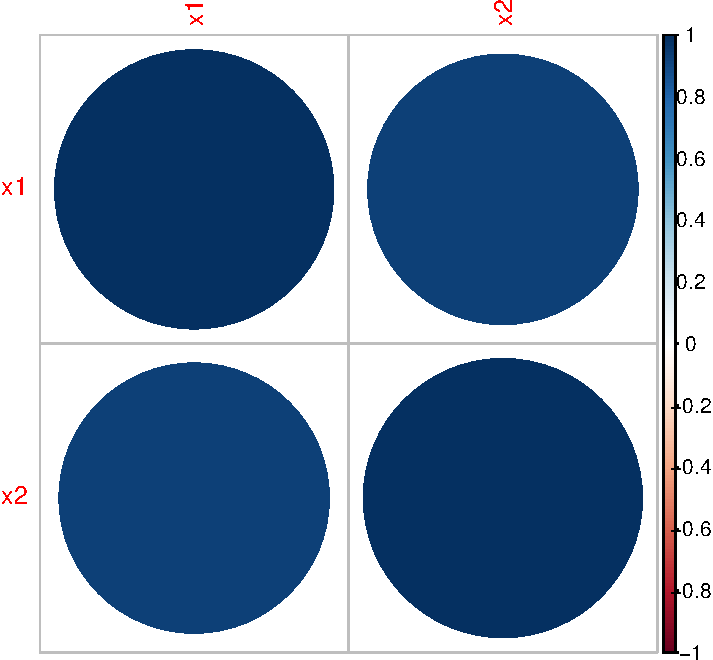
\includegraphics[keepaspectratio]{MultivariateStatisticalAnalysis_files/figure-latex/unnamed-chunk-43-1.pdf}}

Hay una fuerte correlación entre las variables, lo cual es un problema dado que las variables deberían ser independientes.

Vamos a construir dos modelos.

Modelos

\begin{Shaded}
\begin{Highlighting}[]
\NormalTok{modelo1 }\OtherTok{\textless{}{-}} \FunctionTok{lm}\NormalTok{(}\AttributeTok{formula =}\NormalTok{ yp }\SpecialCharTok{\textasciitilde{}}\NormalTok{ x1 }\SpecialCharTok{+}\NormalTok{ x2, }\AttributeTok{data =}\NormalTok{ datos)}

\FunctionTok{summary}\NormalTok{(modelo1)}
\end{Highlighting}
\end{Shaded}

\begin{verbatim}
## 
## Call:
## lm(formula = yp ~ x1 + x2, data = datos)
## 
## Residuals:
##     Min      1Q  Median      3Q     Max 
## -0.8475 -0.3438  0.0043  0.2554  1.1578 
## 
## Coefficients:
##             Estimate Std. Error t value Pr(>|t|)    
## (Intercept)  0.57723    0.59865   0.964    0.367    
## x1           2.70957    0.19935  13.592 2.75e-06 ***
## x2           2.05033    0.04743  43.227 9.26e-10 ***
## ---
## Signif. codes:  0 '***' 0.001 '**' 0.01 '*' 0.05 '.' 0.1 ' ' 1
## 
## Residual standard error: 0.6481 on 7 degrees of freedom
## Multiple R-squared:  0.9997, Adjusted R-squared:  0.9997 
## F-statistic: 1.304e+04 on 2 and 7 DF,  p-value: 3.166e-13
\end{verbatim}

El intercepto parece no ser significativo. Vamos a construir un segundo modelo usando solo \(x_2\) que parece ser más significativa.

Modelo 2

\begin{Shaded}
\begin{Highlighting}[]
\NormalTok{modelo2 }\OtherTok{\textless{}{-}} \FunctionTok{lm}\NormalTok{(}\AttributeTok{formula =}\NormalTok{ yp }\SpecialCharTok{\textasciitilde{}}\NormalTok{ x2, }\AttributeTok{data =}\NormalTok{ datos)}

\FunctionTok{summary}\NormalTok{(modelo2)}
\end{Highlighting}
\end{Shaded}

\begin{verbatim}
## 
## Call:
## lm(formula = yp ~ x2, data = datos)
## 
## Residuals:
##     Min      1Q  Median      3Q     Max 
## -4.0226 -1.7338 -0.3497  1.0695  5.8668 
## 
## Coefficients:
##             Estimate Std. Error t value Pr(>|t|)    
## (Intercept)  7.36967    1.61355   4.567  0.00183 ** 
## x2           2.65476    0.08077  32.869 8.01e-10 ***
## ---
## Signif. codes:  0 '***' 0.001 '**' 0.01 '*' 0.05 '.' 0.1 ' ' 1
## 
## Residual standard error: 3.173 on 8 degrees of freedom
## Multiple R-squared:  0.9926, Adjusted R-squared:  0.9917 
## F-statistic:  1080 on 1 and 8 DF,  p-value: 8.005e-10
\end{verbatim}

El ANOVA nos puede ayudar a ver cual modelo es más significativo. Se usan las hipótesis siguientes:

\(H_0:\) Las variables que eliminamos no tienen significancia.

\(H_1:\) Las variables son significativas.

Si el nuevo modelo es una mejora del modelo original, entonces no podemos rechazar \(H_0\). Si ese no es el caso, significa que esas variables fueron significativas; por lo tanto rechazamos \(H_0\).

ANOVA

\begin{Shaded}
\begin{Highlighting}[]
\FunctionTok{anova}\NormalTok{(modelo1, modelo2)}
\end{Highlighting}
\end{Shaded}

\begin{verbatim}
## Analysis of Variance Table
## 
## Model 1: yp ~ x1 + x2
## Model 2: yp ~ x2
##   Res.Df    RSS Df Sum of Sq      F    Pr(>F)    
## 1      7  2.940                                  
## 2      8 80.532 -1   -77.592 184.74 2.745e-06 ***
## ---
## Signif. codes:  0 '***' 0.001 '**' 0.01 '*' 0.05 '.' 0.1 ' ' 1
\end{verbatim}

Como el p-valor es muy pequeño, menor al valor de significancia 0.05, entonces rechazamos la hipótesis nula, lo que nos dice que el segundo modelo no es una mejora del primero.

Como desde el inicio vimos que el coeficiente correspondiente a \(\beta_0\) no era significativo, vamos a eliminarlo.

Modelo 3

\begin{Shaded}
\begin{Highlighting}[]
\NormalTok{modelo3 }\OtherTok{\textless{}{-}} \FunctionTok{lm}\NormalTok{(}\AttributeTok{formula =}\NormalTok{ yp }\SpecialCharTok{\textasciitilde{}}\NormalTok{ x1 }\SpecialCharTok{+}\NormalTok{ x2 }\SpecialCharTok{{-}}\DecValTok{1}\NormalTok{, }\AttributeTok{data =}\NormalTok{ datos)}

\FunctionTok{summary}\NormalTok{(modelo3)}
\end{Highlighting}
\end{Shaded}

\begin{verbatim}
## 
## Call:
## lm(formula = yp ~ x1 + x2 - 1, data = datos)
## 
## Residuals:
##     Min      1Q  Median      3Q     Max 
## -0.8103 -0.3698  0.1963  0.3955  1.1807 
## 
## Coefficients:
##    Estimate Std. Error t value Pr(>|t|)    
## x1  2.87003    0.10927   26.27 4.74e-09 ***
## x2  2.02140    0.03657   55.28 1.27e-11 ***
## ---
## Signif. codes:  0 '***' 0.001 '**' 0.01 '*' 0.05 '.' 0.1 ' ' 1
## 
## Residual standard error: 0.6452 on 8 degrees of freedom
## Multiple R-squared:  0.9999, Adjusted R-squared:  0.9999 
## F-statistic: 4.188e+04 on 2 and 8 DF,  p-value: < 2.2e-16
\end{verbatim}

\subsection{Normalidad en los residuales}\label{normalidad-en-los-residuales}

Recordemos que los residuos se calculan como la diferencia entre el valor observado \((y)\) y el valor predicho \((\hat{y})\) para cada punto de datos, es decir:

\(e = y - \hat{y}\)

Vamos a hacer un plot de los residuales.

QQ-plot

\begin{Shaded}
\begin{Highlighting}[]
\NormalTok{residuales }\OtherTok{=}\NormalTok{ modelo3}\SpecialCharTok{$}\NormalTok{residuals}

\DocumentationTok{\#\# Q{-}Q plot}
\FunctionTok{qqnorm}\NormalTok{(residuales)}
\FunctionTok{qqline}\NormalTok{(residuales)}
\end{Highlighting}
\end{Shaded}

\pandocbounded{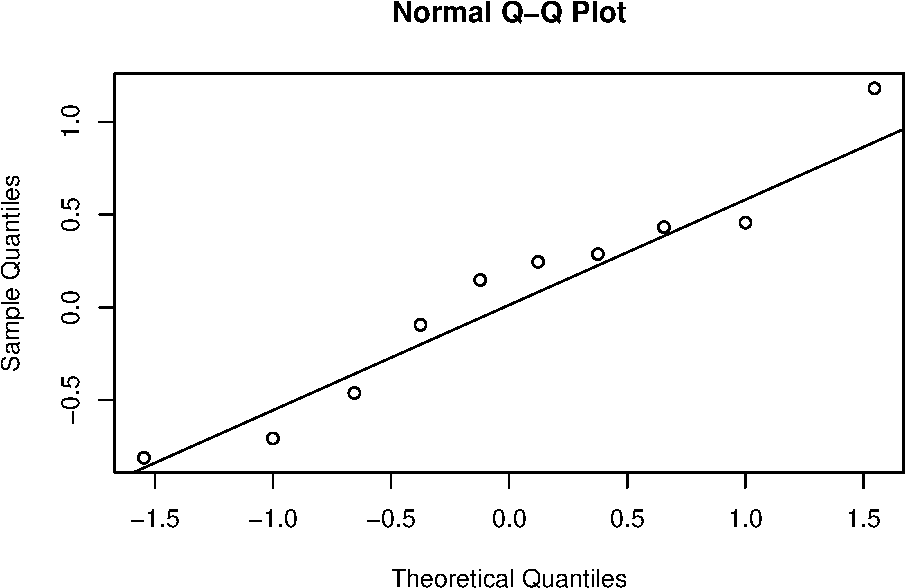
\includegraphics[keepaspectratio]{MultivariateStatisticalAnalysis_files/figure-latex/unnamed-chunk-48-1.pdf}}

Otra forma de obtener este plot es la siguiente.

Plots supuestos

\begin{Shaded}
\begin{Highlighting}[]
\FunctionTok{plot}\NormalTok{(modelo3)}
\end{Highlighting}
\end{Shaded}

\pandocbounded{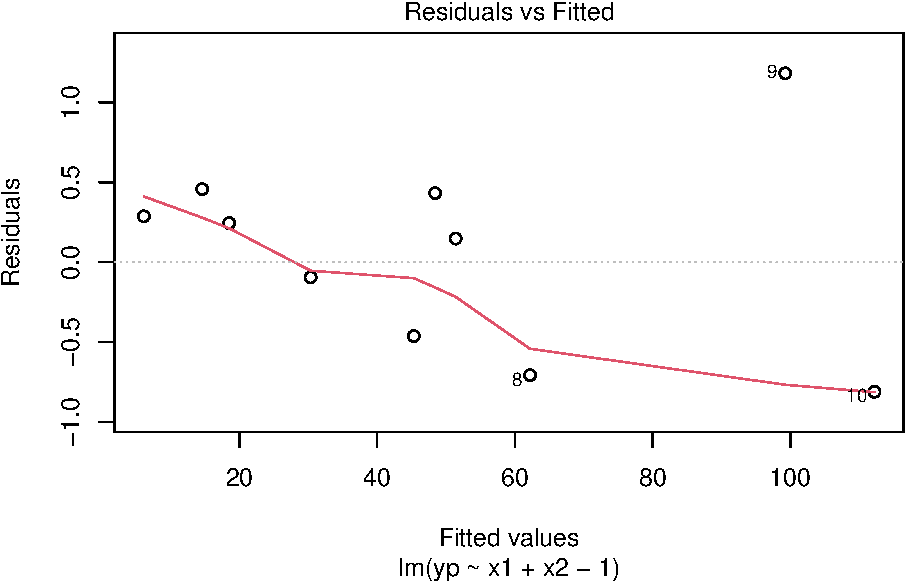
\includegraphics[keepaspectratio]{MultivariateStatisticalAnalysis_files/figure-latex/unnamed-chunk-49-1.pdf}} \pandocbounded{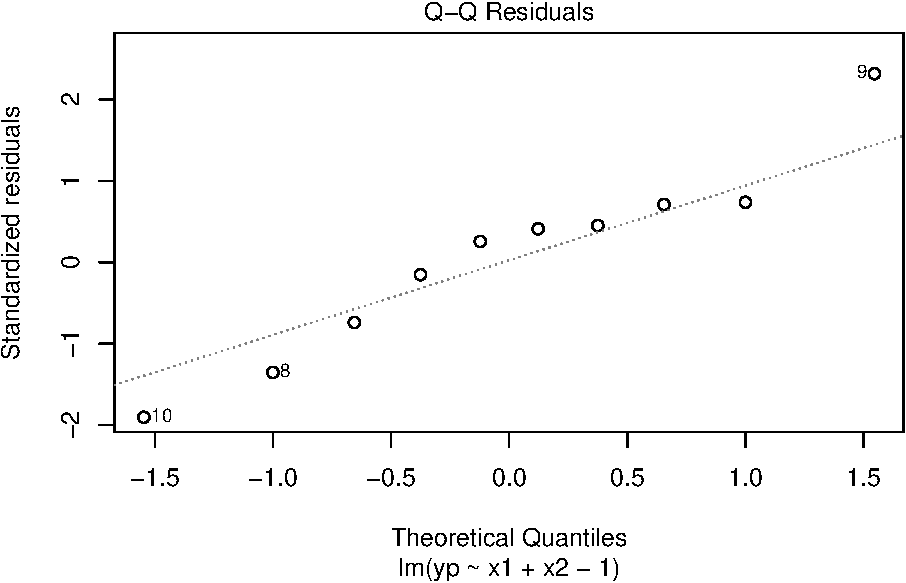
\includegraphics[keepaspectratio]{MultivariateStatisticalAnalysis_files/figure-latex/unnamed-chunk-49-2.pdf}} \pandocbounded{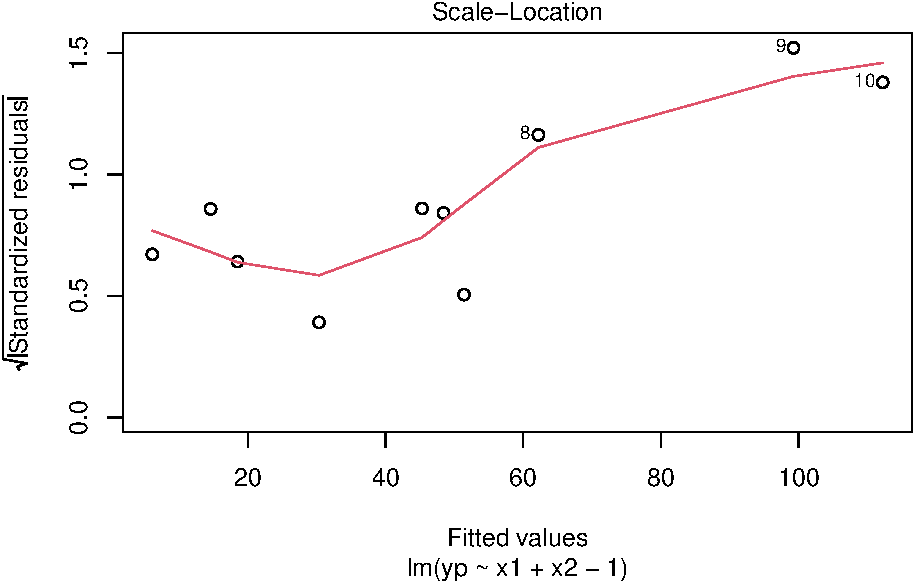
\includegraphics[keepaspectratio]{MultivariateStatisticalAnalysis_files/figure-latex/unnamed-chunk-49-3.pdf}} \pandocbounded{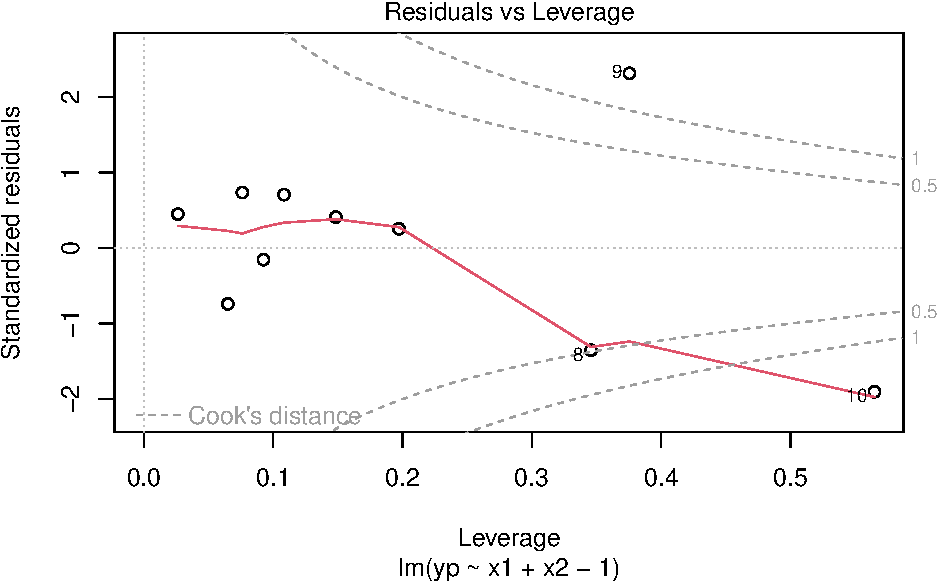
\includegraphics[keepaspectratio]{MultivariateStatisticalAnalysis_files/figure-latex/unnamed-chunk-49-4.pdf}}

El test de Shapiro-Wilks plantea la hipótesis nula que una muestra proviene de una distribución normal. Eligimos un nivel de significanza, por ejemplo \(0.05\), y tenemos una hipótesis alternativa que sostiene que la distribución no es normal. Tenemos entonces lo siguiente:

\(H_0:\) La distribución es normal.

\(H_1:\) La distribución no es normal.

Test Shapiro-Wilks

\begin{Shaded}
\begin{Highlighting}[]
\FunctionTok{shapiro.test}\NormalTok{(residuales)}
\end{Highlighting}
\end{Shaded}

\begin{verbatim}
## 
##  Shapiro-Wilk normality test
## 
## data:  residuales
## W = 0.95058, p-value = 0.6754
\end{verbatim}

Como el p-valor es más grande que el valor de significancia, no podemos rechazar la hipótesis nula, por lo tanto los residuales siguen una distribución normal.

\subsection{Homocedasticidad}\label{homocedasticidad}

Homocedasticidad = varianza constante

\begin{itemize}
\item
  \emph{Correcto:} Si los residuales están dispersos uniformemente a lo largo de todos los valores predichos.
\item
  \emph{Problema:} Si vemos un patrón de embudo (residuales pequeños para predichos bajos y grandes para predichos altos, o viceversa). Esto indica heterocedasticidad.
\end{itemize}

Linealidad y errores independientes: Si se notan curvas, arcos o patrones sistemáticos, podría indicar que:

\begin{itemize}
\item
  La relación no es estrictamente lineal.
\item
  Falta alguna variable importante en el modelo.
\item
  O hay correlación entre errores.
\end{itemize}

Una forma de verlo es con el plot de residuales vs valores predichos.

Plots

\begin{Shaded}
\begin{Highlighting}[]
\FunctionTok{par}\NormalTok{(}\AttributeTok{mfrow =} \FunctionTok{c}\NormalTok{(}\DecValTok{2}\NormalTok{, }\DecValTok{2}\NormalTok{))}
\FunctionTok{plot}\NormalTok{(modelo3)}
\end{Highlighting}
\end{Shaded}

\pandocbounded{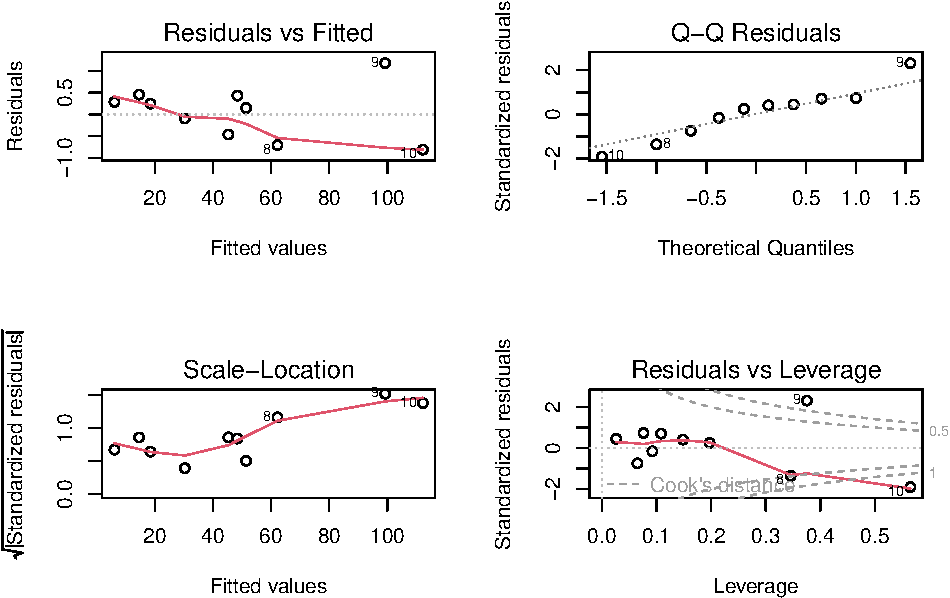
\includegraphics[keepaspectratio]{MultivariateStatisticalAnalysis_files/figure-latex/unnamed-chunk-51-1.pdf}}

En R, existe la función \texttt{bptest()}, que es el test de Breusch-Pagan para la heterocedasticidad. Esta función toma como entrada un modelo de regresión y devuelve el resultado de la prueba de hipótesis para la homocedasticidad de los residuos.

\(H_0:\) los residuos tienen varianza constante (homocedasticidad)

\(H_1\): hay heterocedasticidad en los residuos

El resultado incluye el valor del estadístico de prueba (el valor de la prueba de Breusch-Pagan), el p-valor y el número de grados de libertad. Si el p-valor es menor que el nivel de significancia elegido, se rechaza la hipótesis nula de homocedasticidad y se concluye que hay heterocedasticidad en los residuos.

Breusch-Pagan

\begin{Shaded}
\begin{Highlighting}[]
\FunctionTok{library}\NormalTok{(lmtest)}
\end{Highlighting}
\end{Shaded}

\begin{verbatim}
## Cargando paquete requerido: zoo
\end{verbatim}

\begin{verbatim}
## 
## Adjuntando el paquete: 'zoo'
\end{verbatim}

\begin{verbatim}
## The following objects are masked from 'package:base':
## 
##     as.Date, as.Date.numeric
\end{verbatim}

\begin{Shaded}
\begin{Highlighting}[]
\FunctionTok{bptest}\NormalTok{(modelo3)}
\end{Highlighting}
\end{Shaded}

\begin{verbatim}
## 
##  studentized Breusch-Pagan test
## 
## data:  modelo3
## BP = 5.7517, df = 1, p-value = 0.01647
\end{verbatim}

Entonces como el p-valor es menor al valor de significancia \(0.05\), rechazamos la hipótesis nula y podemos decir que existe heterocedasticidad en los residuales.

La heterocedasticidad es un problema porque la regresión de mínimos cuadrados ordinarios asume que todos los residuales se extraen de una población que tiene una varianza constante (homocedasticidad).

Una forma de corregirlo es haciendo una transformación de los datos. Vamos a transformar la variable \(x_1\).
\emph{Nota:} Estas transformaciones deben de justificarse y explicar el porque.

Modelo 4

\begin{Shaded}
\begin{Highlighting}[]
\NormalTok{modelo4 }\OtherTok{\textless{}{-}} \FunctionTok{lm}\NormalTok{(}\AttributeTok{formula =}\NormalTok{ yp }\SpecialCharTok{\textasciitilde{}} \FunctionTok{log}\NormalTok{(x1) }\SpecialCharTok{+}\NormalTok{ x2 }\SpecialCharTok{{-}}\DecValTok{1}\NormalTok{, }\AttributeTok{data =}\NormalTok{ datos)}

\FunctionTok{summary}\NormalTok{(modelo4)}
\end{Highlighting}
\end{Shaded}

\begin{verbatim}
## 
## Call:
## lm(formula = yp ~ log(x1) + x2 - 1, data = datos)
## 
## Residuals:
##     Min      1Q  Median      3Q     Max 
## -2.4546 -0.7961 -0.3458  0.9207  2.5270 
## 
## Coefficients:
##         Estimate Std. Error t value Pr(>|t|)    
## log(x1)  7.52724    0.72213   10.42 6.22e-06 ***
## x2       2.34013    0.06306   37.11 3.05e-10 ***
## ---
## Signif. codes:  0 '***' 0.001 '**' 0.01 '*' 0.05 '.' 0.1 ' ' 1
## 
## Residual standard error: 1.578 on 8 degrees of freedom
## Multiple R-squared:  0.9994, Adjusted R-squared:  0.9993 
## F-statistic:  6997 on 2 and 8 DF,  p-value: 1.065e-13
\end{verbatim}

Si realizamos la prueba de la homocedasticidad.

Test

\begin{Shaded}
\begin{Highlighting}[]
\FunctionTok{bptest}\NormalTok{(modelo4)}
\end{Highlighting}
\end{Shaded}

\begin{verbatim}
## 
##  studentized Breusch-Pagan test
## 
## data:  modelo4
## BP = 0.13878, df = 1, p-value = 0.7095
\end{verbatim}

Vemos que ahora el p-valor es más grande que el valor de significancia, lo cual nos indica que no podemos rechazar \(H_0\), es decir ahora si podemos asumir que hay homocedasticidad.

En el modelo final, tendríamos \(\beta_0=0\), \(\beta_1*=\) 7.5272361 y \(\beta_2=\) 2.3401283.

Plots finales

\begin{Shaded}
\begin{Highlighting}[]
\FunctionTok{par}\NormalTok{(}\AttributeTok{mfrow =} \FunctionTok{c}\NormalTok{(}\DecValTok{2}\NormalTok{, }\DecValTok{2}\NormalTok{))}
\FunctionTok{plot}\NormalTok{(modelo4)}
\end{Highlighting}
\end{Shaded}

\pandocbounded{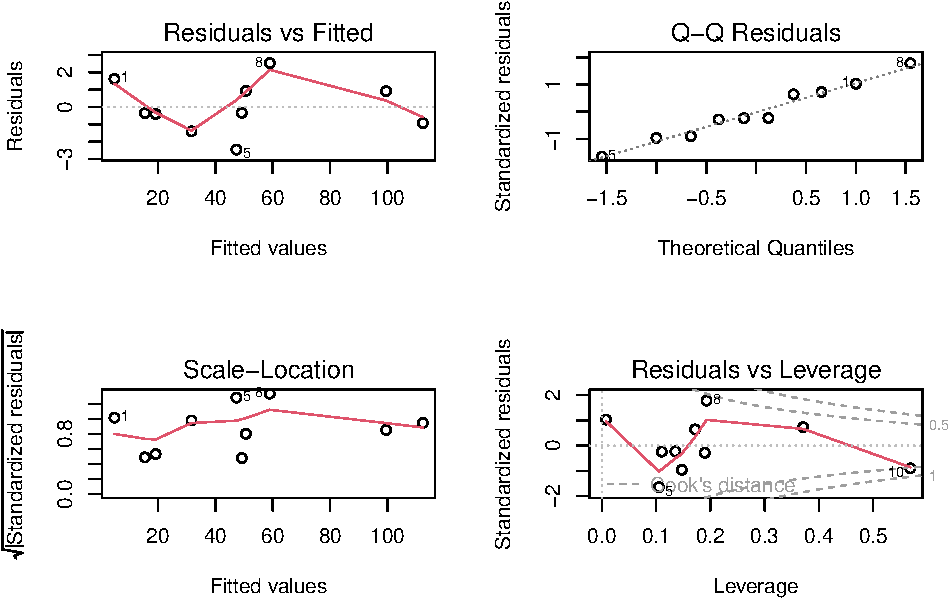
\includegraphics[keepaspectratio]{MultivariateStatisticalAnalysis_files/figure-latex/unnamed-chunk-55-1.pdf}}

Otras dos pruebas que se pueden usar son \texttt{fligner.test} y \texttt{leveneTest}.

\subsection{No autocorrelación}\label{no-autocorrelaciuxf3n}

Una forma de revisar este supuesto es con el test de Durbin-Watson. Las hipótesis que se tienen son:

\(H_0:\) No hay autocorrelación en los errores (los residuales son independientes).

\(H_1:\) Hay autocorrelación en los errores (generalmente, autocorrelación positiva de primer orden).

El estadístico DW toma valores entre 0 y 4:

\begin{itemize}
\item
  \(DW\) aproximadamente 2, entonces no hay autocorrelación (se cumple el supuesto).
\item
  \(DW < 2\), entonces indica autocorrelación positiva (los errores tienden a repetirse).
\item
  \(DW > 2\), entonces indica autocorrelación negativa (los errores tienden a alternar signo).
\end{itemize}

Test D-W

\begin{Shaded}
\begin{Highlighting}[]
\FunctionTok{dwtest}\NormalTok{(modelo4)}
\end{Highlighting}
\end{Shaded}

\begin{verbatim}
## 
##  Durbin-Watson test
## 
## data:  modelo4
## DW = 1.036, p-value = 0.02046
## alternative hypothesis: true autocorrelation is greater than 0
\end{verbatim}

\subsection{Predicciones}\label{predicciones}

Vamos a predecir por último un valor. Para \(2.10\) de ancho del horno y una temperatura de \(3.10\) , ¿cuánto seria el tiempo de cocción?

Predicciónes

\begin{Shaded}
\begin{Highlighting}[]
\NormalTok{nuevo.dato }\OtherTok{\textless{}{-}} \FunctionTok{data.frame}\NormalTok{(}\AttributeTok{x1 =} \FloatTok{2.10}\NormalTok{, }\AttributeTok{x2 =} \FloatTok{3.10}\NormalTok{)}

\NormalTok{prediccion }\OtherTok{\textless{}{-}} \FunctionTok{predict}\NormalTok{(modelo4, }\AttributeTok{newdata =}\NormalTok{ nuevo.dato)}

\FunctionTok{paste}\NormalTok{(}\StringTok{"La cantidad estimada de tiempo de coccion es:"}\NormalTok{, }\FunctionTok{round}\NormalTok{(prediccion, }\DecValTok{2}\NormalTok{))}
\end{Highlighting}
\end{Shaded}

\begin{verbatim}
## [1] "La cantidad estimada de tiempo de coccion es: 12.84"
\end{verbatim}

\subsection{Ejercicios}\label{ejercicios-2}

\textbf{Ejercicio 1:} Para los datos de \texttt{Datarium\ marketing}, analiza los supuestos. Explica tus resultados y sube tus respuestas a github.

\section{Análisis de Varianza}\label{anuxe1lisis-de-varianza}

\textbf{Ejemplo 1: } Supongamos que un cierto tipo de motor de cohete se fabrica uniendo un propulsor tipo A y un propulsor tipo B. La fuerza del enlace entre los dos propulsores es una característica de importancia y se sospecha que está relacionada con la edad (en semanas) del lote del propulsor tipo B. Se tiene una muestra de tamaño 20 de la fuerza del enlace y la edad del lote del propulsor tipo B que fue utilizado.

\begin{Shaded}
\begin{Highlighting}[]
\NormalTok{datos }\OtherTok{\textless{}{-}} \FunctionTok{data.frame}\NormalTok{(}
  \AttributeTok{Fuerza\_enlace =} \FunctionTok{c}\NormalTok{(}
    \FloatTok{2158.70}\NormalTok{, }\FloatTok{1678.15}\NormalTok{, }\FloatTok{2316.00}\NormalTok{, }\FloatTok{2061.30}\NormalTok{, }\FloatTok{2207.50}\NormalTok{,}
    \FloatTok{1708.30}\NormalTok{, }\FloatTok{1784.70}\NormalTok{, }\FloatTok{2575.00}\NormalTok{, }\FloatTok{2357.90}\NormalTok{, }\FloatTok{2256.70}\NormalTok{,}
    \FloatTok{2165.20}\NormalTok{, }\FloatTok{2399.55}\NormalTok{, }\FloatTok{1779.80}\NormalTok{, }\FloatTok{2336.75}\NormalTok{, }\FloatTok{1765.30}\NormalTok{,}
    \FloatTok{2053.50}\NormalTok{, }\FloatTok{2414.40}\NormalTok{, }\FloatTok{2200.50}\NormalTok{, }\FloatTok{2654.20}\NormalTok{, }\FloatTok{1753.70}
\NormalTok{  ),}
  \AttributeTok{Edad\_lote =} \FunctionTok{c}\NormalTok{(}
    \FloatTok{15.50}\NormalTok{, }\FloatTok{23.75}\NormalTok{, }\FloatTok{8.00}\NormalTok{, }\FloatTok{17.00}\NormalTok{, }\FloatTok{5.50}\NormalTok{,}
    \FloatTok{19.00}\NormalTok{, }\FloatTok{24.00}\NormalTok{, }\FloatTok{2.50}\NormalTok{, }\FloatTok{7.50}\NormalTok{, }\FloatTok{11.00}\NormalTok{,}
    \FloatTok{13.00}\NormalTok{, }\FloatTok{3.75}\NormalTok{, }\FloatTok{25.00}\NormalTok{, }\FloatTok{9.75}\NormalTok{, }\FloatTok{22.00}\NormalTok{,}
    \FloatTok{18.00}\NormalTok{, }\FloatTok{6.00}\NormalTok{, }\FloatTok{12.50}\NormalTok{, }\FloatTok{2.00}\NormalTok{, }\FloatTok{21.50}
\NormalTok{  )}
\NormalTok{)}

\NormalTok{datos}
\end{Highlighting}
\end{Shaded}

\begin{verbatim}
##    Fuerza_enlace Edad_lote
## 1        2158.70     15.50
## 2        1678.15     23.75
## 3        2316.00      8.00
## 4        2061.30     17.00
## 5        2207.50      5.50
## 6        1708.30     19.00
## 7        1784.70     24.00
## 8        2575.00      2.50
## 9        2357.90      7.50
## 10       2256.70     11.00
## 11       2165.20     13.00
## 12       2399.55      3.75
## 13       1779.80     25.00
## 14       2336.75      9.75
## 15       1765.30     22.00
## 16       2053.50     18.00
## 17       2414.40      6.00
## 18       2200.50     12.50
## 19       2654.20      2.00
## 20       1753.70     21.50
\end{verbatim}

Un modelo completo sería \(y_i = \beta_0 + \beta_1x_i + \epsilon_i\), el cual se ve como:

\begin{Shaded}
\begin{Highlighting}[]
\NormalTok{modelo\_completo }\OtherTok{\textless{}{-}} \FunctionTok{lm}\NormalTok{(Fuerza\_enlace }\SpecialCharTok{\textasciitilde{}}\NormalTok{ Edad\_lote, }\AttributeTok{data =}\NormalTok{ datos)}

\FunctionTok{plot}\NormalTok{(datos}\SpecialCharTok{$}\NormalTok{Edad\_lote, datos}\SpecialCharTok{$}\NormalTok{Fuerza\_enlace,}
     \AttributeTok{main =} \StringTok{"Modelo completo"}\NormalTok{,}
     \AttributeTok{xlab =} \StringTok{"Edad del lote (semanas)"}\NormalTok{,}
     \AttributeTok{ylab =} \StringTok{"Fuerza del enlace (psi)"}\NormalTok{,}
     \AttributeTok{pch =} \DecValTok{19}\NormalTok{, }\AttributeTok{col =} \StringTok{"blue"}\NormalTok{)}

\CommentTok{\# Agregar la recta de regresión}
\FunctionTok{abline}\NormalTok{(modelo\_completo, }\AttributeTok{col =} \StringTok{"red"}\NormalTok{, }\AttributeTok{lwd =} \DecValTok{2}\NormalTok{)}
\end{Highlighting}
\end{Shaded}

\pandocbounded{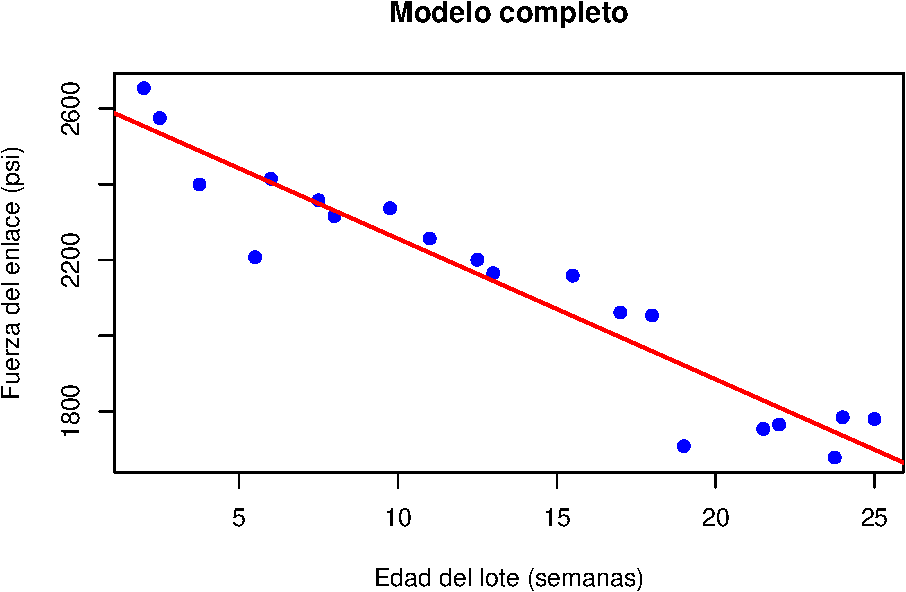
\includegraphics[keepaspectratio]{MultivariateStatisticalAnalysis_files/figure-latex/unnamed-chunk-59-1.pdf}}

\begin{Shaded}
\begin{Highlighting}[]
\FunctionTok{ggplot}\NormalTok{(datos, }\FunctionTok{aes}\NormalTok{(}\AttributeTok{x =}\NormalTok{ Edad\_lote, }\AttributeTok{y =}\NormalTok{ Fuerza\_enlace)) }\SpecialCharTok{+}
  \FunctionTok{geom\_point}\NormalTok{(}\AttributeTok{color =} \StringTok{"blue"}\NormalTok{, }\AttributeTok{size =} \DecValTok{3}\NormalTok{) }\SpecialCharTok{+}
  \FunctionTok{geom\_smooth}\NormalTok{(}\AttributeTok{method =} \StringTok{"lm"}\NormalTok{, }\AttributeTok{se =} \ConstantTok{TRUE}\NormalTok{, }\AttributeTok{color =} \StringTok{"red"}\NormalTok{) }\SpecialCharTok{+}
  \FunctionTok{labs}\NormalTok{(}
    \AttributeTok{title =} \StringTok{"Modelo completo"}\NormalTok{,}
    \AttributeTok{x =} \StringTok{"Edad del lote (semanas)"}\NormalTok{,}
    \AttributeTok{y =} \StringTok{"Fuerza del enlace (psi)"}
\NormalTok{  ) }\SpecialCharTok{+}
  \FunctionTok{theme\_minimal}\NormalTok{()}
\end{Highlighting}
\end{Shaded}

\begin{verbatim}
## `geom_smooth()` using formula = 'y ~ x'
\end{verbatim}

\pandocbounded{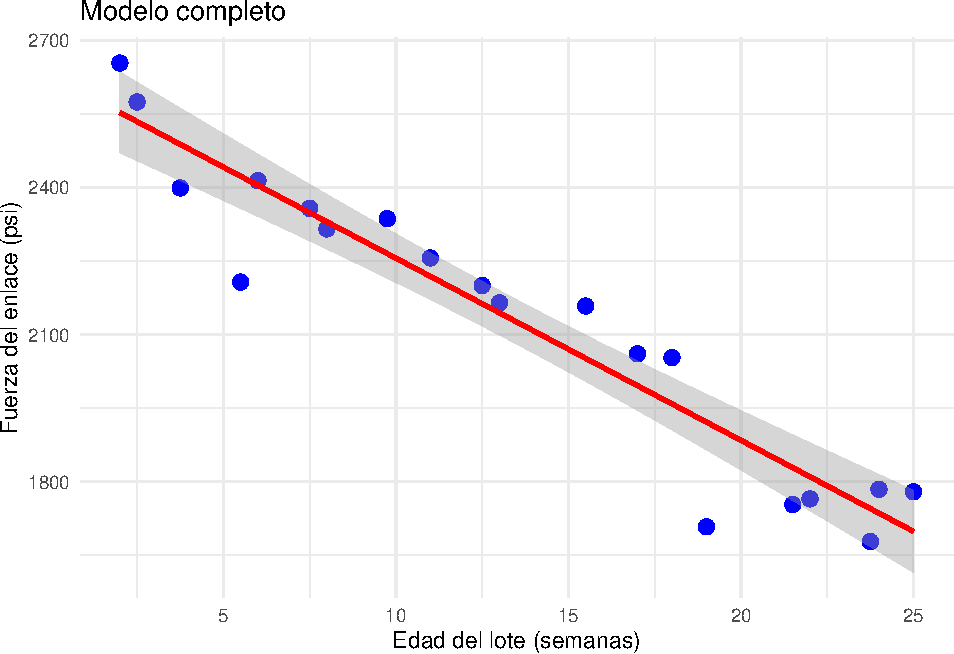
\includegraphics[keepaspectratio]{MultivariateStatisticalAnalysis_files/figure-latex/unnamed-chunk-60-1.pdf}}
Queremos ver si un modelo reducido explica mejor o no a los datos. En este caso el modelo con menos parámetros o modelo reducido es el modelo que describirá la hipótesis nula \(H_0\). En regresión lineal simple, es común plantear \(H_0:\beta_1=0\), de manera que el modelo reducido es \(y_i=\beta_0+\epsilon_i\), es decir, cada valor \(y_i\) es función de una constante (la media) y un error, este modelo se vería como:

\begin{Shaded}
\begin{Highlighting}[]
\NormalTok{modelo\_reducido }\OtherTok{\textless{}{-}} \FunctionTok{lm}\NormalTok{(Fuerza\_enlace }\SpecialCharTok{\textasciitilde{}} \DecValTok{1}\NormalTok{, }\AttributeTok{data =}\NormalTok{ datos)}

\FunctionTok{plot}\NormalTok{(datos}\SpecialCharTok{$}\NormalTok{Edad\_lote, datos}\SpecialCharTok{$}\NormalTok{Fuerza\_enlace,}
     \AttributeTok{main =} \StringTok{"Modelo reducido"}\NormalTok{,}
     \AttributeTok{xlab =} \StringTok{"Edad del lote (semanas)"}\NormalTok{,}
     \AttributeTok{ylab =} \StringTok{"Fuerza del enlace (psi)"}\NormalTok{,}
     \AttributeTok{pch =} \DecValTok{19}\NormalTok{, }\AttributeTok{col =} \StringTok{"blue"}\NormalTok{)}

\CommentTok{\# Agregar la recta de regresión}
\FunctionTok{abline}\NormalTok{(modelo\_reducido, }\AttributeTok{col =} \StringTok{"red"}\NormalTok{, }\AttributeTok{lwd =} \DecValTok{2}\NormalTok{)}
\end{Highlighting}
\end{Shaded}

\pandocbounded{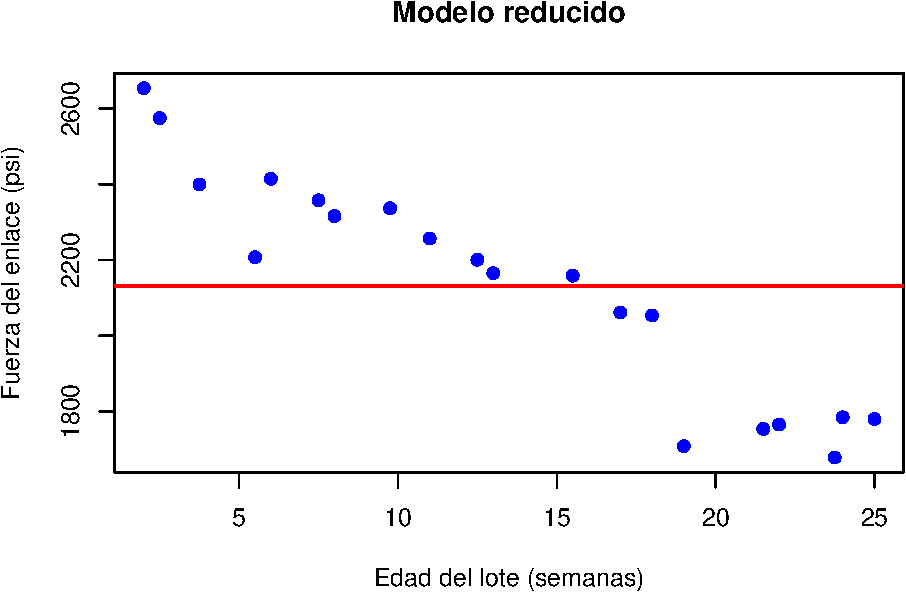
\includegraphics[keepaspectratio]{MultivariateStatisticalAnalysis_files/figure-latex/unnamed-chunk-61-1.pdf}}

\begin{Shaded}
\begin{Highlighting}[]
\FunctionTok{ggplot}\NormalTok{(datos, }\FunctionTok{aes}\NormalTok{(}\AttributeTok{x =}\NormalTok{ Edad\_lote, }\AttributeTok{y =}\NormalTok{ Fuerza\_enlace)) }\SpecialCharTok{+}
  \FunctionTok{geom\_point}\NormalTok{() }\SpecialCharTok{+}
  \FunctionTok{stat\_smooth}\NormalTok{(}\AttributeTok{method =} \StringTok{"lm"}\NormalTok{, }\AttributeTok{formula =}\NormalTok{ y }\SpecialCharTok{\textasciitilde{}} \DecValTok{1}\NormalTok{, }\AttributeTok{se =} \ConstantTok{TRUE}\NormalTok{, }\AttributeTok{fullrange =} \ConstantTok{TRUE}\NormalTok{) }\SpecialCharTok{+}
  \FunctionTok{labs}\NormalTok{(}\AttributeTok{title =} \StringTok{"Modelo reducido"}\NormalTok{,}
       \AttributeTok{x =} \StringTok{"Edad del lote (semanas)"}\NormalTok{, }\AttributeTok{y =} \StringTok{"Fuerza del enlace (psi)"}\NormalTok{) }\SpecialCharTok{+}
  \FunctionTok{theme\_minimal}\NormalTok{()}
\end{Highlighting}
\end{Shaded}

\pandocbounded{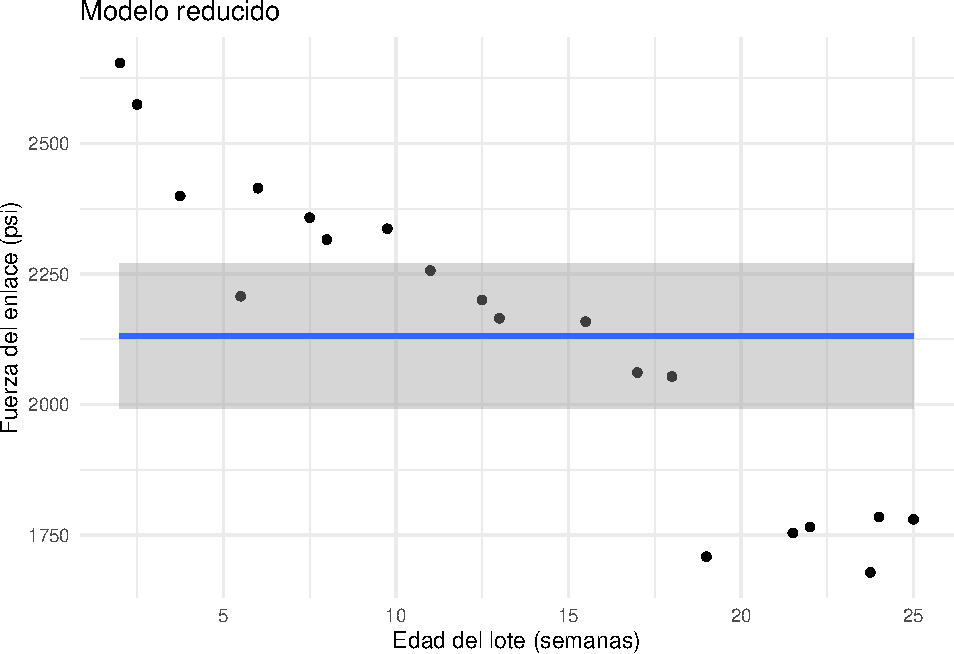
\includegraphics[keepaspectratio]{MultivariateStatisticalAnalysis_files/figure-latex/unnamed-chunk-62-1.pdf}}

¿Cuál modelo es mejor? Debemos obtener los estimadores para cada modelo y la suma de cuadrados de los errores.

\begin{itemize}
\item
  La suma de los cuadrados de los errores \(SSE(C) = \sum(y_i - \hat{y}_i)^2\), la cual tiene \(n-2\) grados de libertad para el modelo completo.
\item
  La suma de los cuadrados de los errores del modelo reducido \(SSE(R) = \sum(y_i - \bar{y}_i)^2\), la cual tiene \(n-1\) grados de libertad para el modelo reducido.
\end{itemize}

Hay que tener en cuenta que \(SSE(R)\) siempre es mayor a \(SSE(C)\), por lo tanto si la diferencia es miu pequeña, entonces tiene sentido utilizar el modelo reducido, pero si la diferencia es muy grande, entonces el parámetro adicional agrega información importante al modelo.

Se usa la prueba \(F\) general:

\[F_0 = \frac{\left( \frac{SSE(R) - SSE(C)}{ (n-1) - (n-2)}  \right)}{\frac{SSE(C)}{n-2}} = \frac{SCE(C)}{\frac{SSE(C)}{n-2}}   \]

La cantidad \(SSE(R) - SSE(C)\) representa la suma de cuadrados explicada por la variable \(x\), a esta cantidad la vamos a denotar por \(SCE\).

Entonces, rechazar la hipótesis nula \(H_0\) implica rechazar el modelo reducido y no rechazar \(H_0\) implica rechazar el modelo completo.

\begin{Shaded}
\begin{Highlighting}[]
\FunctionTok{anova}\NormalTok{(modelo\_completo)}
\end{Highlighting}
\end{Shaded}

\begin{verbatim}
## Analysis of Variance Table
## 
## Response: Fuerza_enlace
##           Df  Sum Sq Mean Sq F value    Pr(>F)    
## Edad_lote  1 1527483 1527483  165.38 1.643e-10 ***
## Residuals 18  166255    9236                      
## ---
## Signif. codes:  0 '***' 0.001 '**' 0.01 '*' 0.05 '.' 0.1 ' ' 1
\end{verbatim}

Como el p-valor es muy pequeño, se rechaza \(H_0\) por lo que se concluye que hay pruebas suficientes sobre la existencia de asociación lineal de la edad de lote y la fuerza del enlace.

Todo esto, se puede llevar al caso de regresión lineal múltiple.

\textbf{Ejemplo:} Considere los siguientes datos en los que se tienen mediciones del tamaño de infarto, área de la región en riesgo y dos variables que identifican el tipo de tratamiento utilizado en 32 pacientes. Se busca describir el tamaño del infarto a través de las otras 3-variables. Para este caso, vamos a ajustar un modelo de regresión lineal múltiple completo y después vamos a hacer pruebas sobre quitar algunas variables.

\begin{Shaded}
\begin{Highlighting}[]
\NormalTok{datos }\OtherTok{\textless{}{-}} \FunctionTok{data.frame}\NormalTok{(}
  \AttributeTok{Paciente =} \DecValTok{1}\SpecialCharTok{:}\DecValTok{32}\NormalTok{,}
  \AttributeTok{Infarc =} \FunctionTok{c}\NormalTok{(}
    \FloatTok{0.119}\NormalTok{, }\FloatTok{0.190}\NormalTok{, }\FloatTok{0.395}\NormalTok{, }\FloatTok{0.469}\NormalTok{, }\FloatTok{0.130}\NormalTok{, }\FloatTok{0.311}\NormalTok{, }\FloatTok{0.418}\NormalTok{, }\FloatTok{0.480}\NormalTok{,}
    \FloatTok{0.687}\NormalTok{, }\FloatTok{0.847}\NormalTok{, }\FloatTok{0.062}\NormalTok{, }\FloatTok{0.122}\NormalTok{, }\FloatTok{0.033}\NormalTok{, }\FloatTok{0.102}\NormalTok{, }\FloatTok{0.206}\NormalTok{, }\FloatTok{0.249}\NormalTok{,}
    \FloatTok{0.220}\NormalTok{, }\FloatTok{0.299}\NormalTok{, }\FloatTok{0.350}\NormalTok{, }\FloatTok{0.350}\NormalTok{, }\FloatTok{0.588}\NormalTok{, }\FloatTok{0.379}\NormalTok{, }\FloatTok{0.149}\NormalTok{, }\FloatTok{0.316}\NormalTok{,}
    \FloatTok{0.390}\NormalTok{, }\FloatTok{0.429}\NormalTok{, }\FloatTok{0.477}\NormalTok{, }\FloatTok{0.439}\NormalTok{, }\FloatTok{0.446}\NormalTok{, }\FloatTok{0.538}\NormalTok{, }\FloatTok{0.625}\NormalTok{, }\FloatTok{0.974}
\NormalTok{  ),}
  \AttributeTok{Area =} \FunctionTok{c}\NormalTok{(}
    \FloatTok{0.34}\NormalTok{, }\FloatTok{0.64}\NormalTok{, }\FloatTok{0.76}\NormalTok{, }\FloatTok{0.83}\NormalTok{, }\FloatTok{0.73}\NormalTok{, }\FloatTok{0.82}\NormalTok{, }\FloatTok{0.95}\NormalTok{, }\FloatTok{1.06}\NormalTok{,}
    \FloatTok{1.20}\NormalTok{, }\FloatTok{1.47}\NormalTok{, }\FloatTok{0.44}\NormalTok{, }\FloatTok{0.77}\NormalTok{, }\FloatTok{0.90}\NormalTok{, }\FloatTok{1.07}\NormalTok{, }\FloatTok{1.01}\NormalTok{, }\FloatTok{1.03}\NormalTok{,}
    \FloatTok{1.16}\NormalTok{, }\FloatTok{1.21}\NormalTok{, }\FloatTok{1.20}\NormalTok{, }\FloatTok{1.22}\NormalTok{, }\FloatTok{0.99}\NormalTok{, }\FloatTok{0.77}\NormalTok{, }\FloatTok{1.05}\NormalTok{, }\FloatTok{1.06}\NormalTok{,}
    \FloatTok{1.02}\NormalTok{, }\FloatTok{0.99}\NormalTok{, }\FloatTok{0.97}\NormalTok{, }\FloatTok{1.12}\NormalTok{, }\FloatTok{1.23}\NormalTok{, }\FloatTok{1.19}\NormalTok{, }\FloatTok{1.22}\NormalTok{, }\FloatTok{1.40}
\NormalTok{  ),}
  \AttributeTok{X2 =} \FunctionTok{c}\NormalTok{(}
    \DecValTok{0}\NormalTok{,}\DecValTok{0}\NormalTok{,}\DecValTok{0}\NormalTok{,}\DecValTok{0}\NormalTok{,}\DecValTok{0}\NormalTok{,}\DecValTok{0}\NormalTok{,}\DecValTok{0}\NormalTok{,}\DecValTok{0}\NormalTok{,}
    \DecValTok{0}\NormalTok{,}\DecValTok{0}\NormalTok{,}\DecValTok{1}\NormalTok{,}\DecValTok{1}\NormalTok{,}\DecValTok{1}\NormalTok{,}\DecValTok{1}\NormalTok{,}\DecValTok{1}\NormalTok{,}\DecValTok{1}\NormalTok{,}
    \DecValTok{1}\NormalTok{,}\DecValTok{1}\NormalTok{,}\DecValTok{1}\NormalTok{,}\DecValTok{1}\NormalTok{,}\DecValTok{1}\NormalTok{,}\DecValTok{0}\NormalTok{,}\DecValTok{0}\NormalTok{,}\DecValTok{0}\NormalTok{,}
    \DecValTok{0}\NormalTok{,}\DecValTok{0}\NormalTok{,}\DecValTok{0}\NormalTok{,}\DecValTok{0}\NormalTok{,}\DecValTok{0}\NormalTok{,}\DecValTok{0}\NormalTok{,}\DecValTok{0}\NormalTok{,}\DecValTok{0}
\NormalTok{  ),}
  \AttributeTok{X3 =} \FunctionTok{c}\NormalTok{(}
    \DecValTok{0}\NormalTok{,}\DecValTok{0}\NormalTok{,}\DecValTok{0}\NormalTok{,}\DecValTok{0}\NormalTok{,}\DecValTok{0}\NormalTok{,}\DecValTok{0}\NormalTok{,}\DecValTok{0}\NormalTok{,}\DecValTok{0}\NormalTok{,}
    \DecValTok{0}\NormalTok{,}\DecValTok{0}\NormalTok{,}\DecValTok{0}\NormalTok{,}\DecValTok{0}\NormalTok{,}\DecValTok{0}\NormalTok{,}\DecValTok{0}\NormalTok{,}\DecValTok{0}\NormalTok{,}\DecValTok{0}\NormalTok{,}
    \DecValTok{0}\NormalTok{,}\DecValTok{0}\NormalTok{,}\DecValTok{0}\NormalTok{,}\DecValTok{0}\NormalTok{,}\DecValTok{0}\NormalTok{,}\DecValTok{0}\NormalTok{,}\DecValTok{1}\NormalTok{,}\DecValTok{1}\NormalTok{,}
    \DecValTok{1}\NormalTok{,}\DecValTok{1}\NormalTok{,}\DecValTok{1}\NormalTok{,}\DecValTok{1}\NormalTok{,}\DecValTok{1}\NormalTok{,}\DecValTok{1}\NormalTok{,}\DecValTok{1}\NormalTok{,}\DecValTok{1}
\NormalTok{  )}
\NormalTok{)}
\NormalTok{datos}
\end{Highlighting}
\end{Shaded}

\begin{verbatim}
##    Paciente Infarc Area X2 X3
## 1         1  0.119 0.34  0  0
## 2         2  0.190 0.64  0  0
## 3         3  0.395 0.76  0  0
## 4         4  0.469 0.83  0  0
## 5         5  0.130 0.73  0  0
## 6         6  0.311 0.82  0  0
## 7         7  0.418 0.95  0  0
## 8         8  0.480 1.06  0  0
## 9         9  0.687 1.20  0  0
## 10       10  0.847 1.47  0  0
## 11       11  0.062 0.44  1  0
## 12       12  0.122 0.77  1  0
## 13       13  0.033 0.90  1  0
## 14       14  0.102 1.07  1  0
## 15       15  0.206 1.01  1  0
## 16       16  0.249 1.03  1  0
## 17       17  0.220 1.16  1  0
## 18       18  0.299 1.21  1  0
## 19       19  0.350 1.20  1  0
## 20       20  0.350 1.22  1  0
## 21       21  0.588 0.99  1  0
## 22       22  0.379 0.77  0  0
## 23       23  0.149 1.05  0  1
## 24       24  0.316 1.06  0  1
## 25       25  0.390 1.02  0  1
## 26       26  0.429 0.99  0  1
## 27       27  0.477 0.97  0  1
## 28       28  0.439 1.12  0  1
## 29       29  0.446 1.23  0  1
## 30       30  0.538 1.19  0  1
## 31       31  0.625 1.22  0  1
## 32       32  0.974 1.40  0  1
\end{verbatim}

El modelo completo sería \(y_i = \beta_0 + \beta_1x_{1i} +\beta_2x_{2i} + \beta_3x_{3i}+\epsilon_i\).

\begin{Shaded}
\begin{Highlighting}[]
\NormalTok{modelo\_c }\OtherTok{\textless{}{-}} \FunctionTok{lm}\NormalTok{(Infarc}\SpecialCharTok{\textasciitilde{}}\NormalTok{ Area }\SpecialCharTok{+}\NormalTok{ X2 }\SpecialCharTok{+}\NormalTok{ X3, }\AttributeTok{data =}\NormalTok{ datos)}
\FunctionTok{summary}\NormalTok{(modelo\_c)}
\end{Highlighting}
\end{Shaded}

\begin{verbatim}
## 
## Call:
## lm(formula = Infarc ~ Area + X2 + X3, data = datos)
## 
## Residuals:
##      Min       1Q   Median       3Q      Max 
## -0.28175 -0.06704 -0.01658  0.06294  0.35970 
## 
## Coefficients:
##             Estimate Std. Error t value Pr(>|t|)    
## (Intercept) -0.14927    0.10377  -1.439 0.161376    
## Area         0.63395    0.10927   5.802 3.12e-06 ***
## X2          -0.25005    0.06053  -4.131 0.000295 ***
## X3          -0.08563    0.06641  -1.289 0.207831    
## ---
## Signif. codes:  0 '***' 0.001 '**' 0.01 '*' 0.05 '.' 0.1 ' ' 1
## 
## Residual standard error: 0.138 on 28 degrees of freedom
## Multiple R-squared:  0.6456, Adjusted R-squared:  0.6076 
## F-statistic:    17 on 3 and 28 DF,  p-value: 1.748e-06
\end{verbatim}

Con este modelo se obtiene la siguiente tabla de ANOVA.

\begin{Shaded}
\begin{Highlighting}[]
\NormalTok{anov }\OtherTok{\textless{}{-}} \FunctionTok{anova}\NormalTok{(modelo\_c)}
\NormalTok{anov}
\end{Highlighting}
\end{Shaded}

\begin{verbatim}
## Analysis of Variance Table
## 
## Response: Infarc
##           Df  Sum Sq Mean Sq F value    Pr(>F)    
## Area       1 0.62492 0.62492 32.8245 3.801e-06 ***
## X2         1 0.31453 0.31453 16.5210 0.0003533 ***
## X3         1 0.03165 0.03165  1.6624 0.2078307    
## Residuals 28 0.53307 0.01904                      
## ---
## Signif. codes:  0 '***' 0.001 '**' 0.01 '*' 0.05 '.' 0.1 ' ' 1
\end{verbatim}

\begin{Shaded}
\begin{Highlighting}[]
\DocumentationTok{\#\# los p{-}valores en la última columna se pueden obtener con: }
\CommentTok{\#pf(F\_0, df1, df2, lower.tail = FALSE)}
\end{Highlighting}
\end{Shaded}

\textbf{1) Pruebas sobre uno de los parámetros:} \(H_0:\beta_1=0\), modelo reducido \(y_i = \beta_0  +\beta_2x_{2i} + \beta_3x_{3i}+\epsilon_i\). Vamos a denotar a la suma de los cuadrados de los errores asociada a este modelo \(SSE(x_1)\), la cual tiene \(n-3\) grados de libertad asociados (tenemos 3 parámetros a estimar \(\beta_0,\beta_2,\beta_3\)). Como el p-valor es muy pequeño, se rechaza a \(H_0\) y se concluye que hay suficiente evidencia para decir que el tamaño del infarto está significativamente relacionado con el tamaño del área de riesgo.

\begin{Shaded}
\begin{Highlighting}[]
\NormalTok{SCE\_X1 }\OtherTok{\textless{}{-}}\NormalTok{ anov}\SpecialCharTok{$}\StringTok{\textasciigrave{}}\AttributeTok{Sum Sq}\StringTok{\textasciigrave{}}\NormalTok{[}\DecValTok{1}\NormalTok{]}
\NormalTok{SSE\_C }\OtherTok{\textless{}{-}}\NormalTok{ anov}\SpecialCharTok{$}\StringTok{\textasciigrave{}}\AttributeTok{Sum Sq}\StringTok{\textasciigrave{}}\NormalTok{[}\DecValTok{4}\NormalTok{]}
\NormalTok{df2 }\OtherTok{\textless{}{-}}\NormalTok{ anov}\SpecialCharTok{$}\NormalTok{Df[}\DecValTok{4}\NormalTok{]}
\NormalTok{df1 }\OtherTok{\textless{}{-}} \FunctionTok{nrow}\NormalTok{(datos) }\SpecialCharTok{{-}} \DecValTok{3} \SpecialCharTok{{-}}\NormalTok{ df2}
\NormalTok{F\_g }\OtherTok{\textless{}{-}}\NormalTok{ (SCE\_X1}\SpecialCharTok{/}\NormalTok{df1) }\SpecialCharTok{/}\NormalTok{ (SSE\_C}\SpecialCharTok{/}\NormalTok{df2) }
\NormalTok{F\_g}
\end{Highlighting}
\end{Shaded}

\begin{verbatim}
## [1] 32.82447
\end{verbatim}

\textbf{2) Pruebas sobre todos los parámetros:} En este caso tenemos \(H_0:\beta_1=\beta_2=\beta_3=0\) vs \(H_1: \beta_j\neq 0\) p.a. \(j\). Es decir, el modelo reducido sería \(y_i = \beta_0+\epsilon_i\). La prueba \(F\) general es la misma, pero ahora la suma de cuadrados asociada al modelo reducido \(SSE(x_1,x_2,x_3)\) tiene \(n-1\) grados de libertad ya que solo debemos estimar \(\beta_0\).

\begin{Shaded}
\begin{Highlighting}[]
\NormalTok{SCE\_X1X2X3 }\OtherTok{\textless{}{-}} \FunctionTok{sum}\NormalTok{(anov}\SpecialCharTok{$}\StringTok{\textasciigrave{}}\AttributeTok{Sum Sq}\StringTok{\textasciigrave{}}\NormalTok{[}\DecValTok{1}\SpecialCharTok{:}\DecValTok{3}\NormalTok{]) }
\NormalTok{df1 }\OtherTok{\textless{}{-}} \FunctionTok{nrow}\NormalTok{(datos) }\SpecialCharTok{{-}}\DecValTok{1} \SpecialCharTok{{-}}\NormalTok{ df2 }

\NormalTok{F\_all }\OtherTok{\textless{}{-}}\NormalTok{ (SCE\_X1X2X3 }\SpecialCharTok{/}\NormalTok{ df1) }\SpecialCharTok{/}\NormalTok{ (SSE\_C }\SpecialCharTok{/}\NormalTok{ df2)}
\NormalTok{F\_all}
\end{Highlighting}
\end{Shaded}

\begin{verbatim}
## [1] 17.00263
\end{verbatim}

El cual tiene un \(p-\)valor asociado a una distribución \(F\) con 3 y 28 grados de libertad.

\begin{Shaded}
\begin{Highlighting}[]
\FunctionTok{pf}\NormalTok{(F\_all, }\AttributeTok{df1 =} \DecValTok{3}\NormalTok{, }\AttributeTok{df2 =} \DecValTok{28}\NormalTok{, }\AttributeTok{lower.tail =} \ConstantTok{FALSE}\NormalTok{)}
\end{Highlighting}
\end{Shaded}

\begin{verbatim}
## [1] 1.747583e-06
\end{verbatim}

Por lo tanto rechazamos la hipótesis nula. Notemos que este valor coincide con el que nos da el \texttt{summary} del modelo.

\begin{Shaded}
\begin{Highlighting}[]
\FunctionTok{summary}\NormalTok{(modelo\_c)}
\end{Highlighting}
\end{Shaded}

\begin{verbatim}
## 
## Call:
## lm(formula = Infarc ~ Area + X2 + X3, data = datos)
## 
## Residuals:
##      Min       1Q   Median       3Q      Max 
## -0.28175 -0.06704 -0.01658  0.06294  0.35970 
## 
## Coefficients:
##             Estimate Std. Error t value Pr(>|t|)    
## (Intercept) -0.14927    0.10377  -1.439 0.161376    
## Area         0.63395    0.10927   5.802 3.12e-06 ***
## X2          -0.25005    0.06053  -4.131 0.000295 ***
## X3          -0.08563    0.06641  -1.289 0.207831    
## ---
## Signif. codes:  0 '***' 0.001 '**' 0.01 '*' 0.05 '.' 0.1 ' ' 1
## 
## Residual standard error: 0.138 on 28 degrees of freedom
## Multiple R-squared:  0.6456, Adjusted R-squared:  0.6076 
## F-statistic:    17 on 3 and 28 DF,  p-value: 1.748e-06
\end{verbatim}

\textbf{3) Pruebas sobre un subconjunto de los parámetros:} Supongamos ahora que \(H_0:\beta_2=\beta_3=0\). Es decir, el modelo reducido sería \(y_i = \beta_0+ \beta_1x_{1i}+\epsilon_i\). La prueba es similar pero solo usamos \(x_2\) y \(x_3\).

\begin{Shaded}
\begin{Highlighting}[]
\NormalTok{SCE\_X2X3 }\OtherTok{\textless{}{-}} \FunctionTok{sum}\NormalTok{(anov}\SpecialCharTok{$}\StringTok{\textasciigrave{}}\AttributeTok{Sum Sq}\StringTok{\textasciigrave{}}\NormalTok{[}\DecValTok{2}\SpecialCharTok{:}\DecValTok{3}\NormalTok{]) }
\NormalTok{df1 }\OtherTok{\textless{}{-}} \FunctionTok{nrow}\NormalTok{(datos) }\SpecialCharTok{{-}} \DecValTok{2} \SpecialCharTok{{-}}\NormalTok{ df2 }

\NormalTok{F\_dos }\OtherTok{\textless{}{-}}\NormalTok{ (SCE\_X2X3 }\SpecialCharTok{/}\NormalTok{ df1) }\SpecialCharTok{/}\NormalTok{ (SSE\_C }\SpecialCharTok{/}\NormalTok{ df2)}
\NormalTok{F\_dos}
\end{Highlighting}
\end{Shaded}

\begin{verbatim}
## [1] 9.091716
\end{verbatim}

El \(p-\)valor asociado a la prueba \(F\) con 2 y 28 grados de libertad es:

\begin{Shaded}
\begin{Highlighting}[]
\FunctionTok{pf}\NormalTok{(F\_dos, }\AttributeTok{df1 =} \DecValTok{2}\NormalTok{, }\AttributeTok{df2 =} \DecValTok{28}\NormalTok{, }\AttributeTok{lower.tail =} \ConstantTok{FALSE}\NormalTok{)}
\end{Highlighting}
\end{Shaded}

\begin{verbatim}
## [1] 0.0009065789
\end{verbatim}

Por lo que se rechaza de nuevo la hipótesis nula.

\subsection{Ejercicios}\label{ejercicios-3}

\textbf{Ejercicio 1(R):} Para el datasets \texttt{datasets::trees}, realice las pruebas de hipótesis para determinar si:
1) El modelo solo con la variable \texttt{Girth} es mejor que el modelo completo.
2) El modelo sin \texttt{Girth} y \texttt{Height} es mejor que el completo.
Usar la tabla de ANOVA para calcular el estadístico \(F_0\) y encontrar el p-valor asociado usando \texttt{pf(F\_0,\ df1,\ df2,\ lower.tail\ =\ FALSE)}. Justifique su respuesta y suba su código en R a github.

\textbf{Ejercicio 2(Python):} Para el dataset de \texttt{marketing}, realice las pruebas de hipótesis utilizando la tabla de ANOVA sobre:
1) Uno de los parámetros, justificar cual.
2) Todos los parámetros.
3)Un subconjunto de parámetros, justificar cual.
Usar la tabla de ANOVA para calcular el estadístico \(F_0\) y encontrar el p-valor asociado usando \texttt{pf(F\_0,\ df1,\ df2,\ lower.tail\ =\ FALSE)}. Justifique su respuesta y suba su código en Python a github.

\section{Selección del modelo}\label{selecciuxf3n-del-modelo}

Suponga que se busca una ecuación de regresión lineal entre la variable respuesta \(y\) y las variables predictoras \(x_1,...,x_p\). Suponga que se tiene el conjunto de todas las posibles variables a incluir en el modelo \(z_1,...z_k\) que son funciones de las \(x\)'s. Se busca entonces un modelo que incluya la mayor cantidad de variables \(z\) posible para que el error sea pequeño. Pero, considerando la varianza y el costo de obtener más datos, también se busca incluir el menor número de posibles variables \(z\) en el modelo.

No existe un solo método de selección de modelos y no todos conducen a la misma solución. Vamos a analizar tres métodos:

\begin{enumerate}
\def\labelenumi{\arabic{enumi})}
\tightlist
\item
  Todos los modelos posibles y el mejor subconjunto de modelos.
\item
  Selección paso a paso.
\item
  Eliminación hacia atrás.
\end{enumerate}

\subsection{Todos los modelos posibles}\label{todos-los-modelos-posibles}

Si el número de variables \(z\) es grande, esto puede ser un problema. Supongamos que tenemos \(k\) variables, donde cada variable puede o no estar en el modelo, entonces tenemos un total de \(2^k\) posibles modelos de los cuales se debe elegir el mejor a partir de criterios como \(R^2\), \(R^2_{adj}\), etc. Vamos a ver algunos de estos criterios.

\textbf{Estadística \(C_p\) de Mallows}

Supongamos que tenemos \(k+1\) variables regresoras incluyendo el intercepto, de las cuales vamos a elegir \(p\). Denotemos por \(SSE_p\) la suma de cuadrados de la regresión respectiva de tomar \(p\) variables, la estadística \(C_p\) de Mallows está dada por

\[C_p = \frac{SSE_p}{\hat{\sigma}^2} - (n-2p)  \]
donde \(\hat{\sigma}^2\) corresponde al modelo con todas las variables y se supone que es un estimador insesgado para la varianza \(\sigma^2\). Si el modelo ajusta bien, esperaríamos que \(\mathbb{E}(SSE_p)=(n-p)\sigma^2\), de manera que:

\[\mathbb{E}(C_p)\approx p,\]

en consecuencia, si graficamos \(C_p\) en función de \(p\), los modelos adecuados arrojarán puntos cerca de la recta \(C_p=p\).

\textbf{Criterio de información de Akaike (CIA)}

Se define como

\[CIA = e^{\frac{2p}{n}}\frac{SSE}{n},\]

donde \(p\) es el número de variables regresoras incluyendo el intercepto. Esta función incluye una penalización por imponer regresoras. Al comparar modelos, se busca el que tenga menor \(CIA\). Muchas veces esta estadística se define como \(\log(CIA)\), es decir:

\[\frac{2p}{n}+\log(\frac{SSE}{n})\]

con el cual las conclusiones son las mismas.

\textbf{Criterio de información de Schwars (CIS)}

Similar al CIA, el CIS se define como

\[CIS = n^{\frac{p}{n}}\frac{SSE}{n},\]

cuyo logaritmo es

\[\frac{p}{n}\log{n} + \log{\frac{SSE}{n}}.\]

Este criterio impone mayor penalización por agregar variables. Al comparar modelos, se busca el que tenga menor CIS.

\subsubsection{Mejor subconjunto}\label{mejor-subconjunto}

Una alternativa a la comparación de todos los modelos posibles es la búsqueda del mejor subconjunto de modelos que se pueden hacer en distintos programas y compararlos. En R, existe la función \texttt{regsubsets}, la cual incluye los criterios de comparación \(R^2, C_p,\) BIC (Bayesian Information Criterion). Esta función utiliza los métodos \emph{forward and backward stepwise}.

\subsection{Selección paso a paso}\label{selecciuxf3n-paso-a-paso}

Las técnicas de selección paso a paso consisten en elaborar un modelo inicial a partir del cual se agrega o se elimina una variable para comparar hasta encontrar el mejor modelo.

\subsubsection{Selección paso a paso hacia adelante}\label{selecciuxf3n-paso-a-paso-hacia-adelante}

Conocido como \emph{forward regression}, consiste en comenzar con el modelo en el que la única variable regresora es la que mejor describe el comportamiento de \(y\) y a partir de ahí ir agregando variables regresoras una por una.

El orden en el que se agregan puede variar y se pueden usar diferentes estadísticas o criterios para decidir cual agregar. Se calculan las estadísticas del modelo actual al agregar variable y elegir el modelo con la mejor estadística, siempre que sea un mejor modelo.

\subsubsection{Selección paso a paso hacia atrás}\label{selecciuxf3n-paso-a-paso-hacia-atruxe1s}

Conocido como \emph{backward regression}, consiste en comenzar con el modelo que incluye todas las variables e ir eliminando una a una de acuerdo a algún criterio.

Ambas técnicas se pueden mezclar, de manera que en cada paso se evalúa la estadística correspondiente al quitar o agregar alguna de las variables y se elige la mejor opción.

\subsection{Ejemplos}\label{ejemplos}

\subsubsection{Todos los modelos posibles}\label{todos-los-modelos-posibles-1}

En este ejemplo veremos cómo aplicar el método de seleccion de modelos que implica el análisis de todos los modelos posibles. Primero, necesitaremos varios paquetes.

\begin{Shaded}
\begin{Highlighting}[]
\FunctionTok{library}\NormalTok{(ggplot2)}
\FunctionTok{library}\NormalTok{(olsrr)}
\end{Highlighting}
\end{Shaded}

\begin{verbatim}
## 
## Adjuntando el paquete: 'olsrr'
\end{verbatim}

\begin{verbatim}
## The following object is masked from 'package:datasets':
## 
##     rivers
\end{verbatim}

\begin{Shaded}
\begin{Highlighting}[]
\FunctionTok{library}\NormalTok{(leaps)}
\FunctionTok{library}\NormalTok{(GGally)}
\end{Highlighting}
\end{Shaded}

\textbf{Ejemplo 1:} Cargamos los datos de \texttt{cemento.txt} y hacemos un rápido análisis con el diagrama de dispersión:

\begin{Shaded}
\begin{Highlighting}[]
\NormalTok{cemento}\OtherTok{\textless{}{-}}\FunctionTok{read.table}\NormalTok{(}\StringTok{"D:/Users/hayde/Documents/R\_sites/MultivariateStatisticalAnalysis/data/cement.txt"}\NormalTok{, }\AttributeTok{header =}\NormalTok{ T, }\AttributeTok{skip=}\DecValTok{5}\NormalTok{)}
\FunctionTok{ggpairs}\NormalTok{(cemento)}
\end{Highlighting}
\end{Shaded}

\pandocbounded{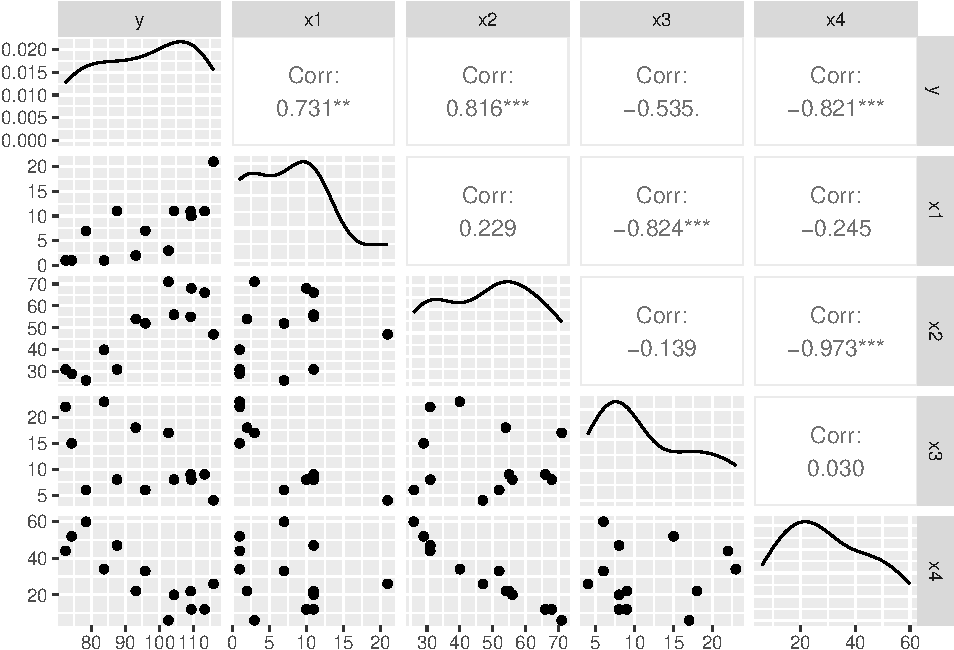
\includegraphics[keepaspectratio]{MultivariateStatisticalAnalysis_files/figure-latex/unnamed-chunk-74-1.pdf}}

A continuación ajustamos el modelo con TODAS las variables independientes y calculamos la estadística \(C_p\). Para facilitar la interpretación graficamos la \(C_p\) para cada modelo:

\begin{Shaded}
\begin{Highlighting}[]
\NormalTok{modelo.full}\OtherTok{\textless{}{-}}\FunctionTok{lm}\NormalTok{(y}\SpecialCharTok{\textasciitilde{}}\NormalTok{., cemento, }\AttributeTok{x=}\NormalTok{T, }\AttributeTok{y=}\NormalTok{T)}
\DocumentationTok{\#\# calcula el AIC, CIS, etc sobre todos los subconjuntos posibles}
\NormalTok{outs}\OtherTok{\textless{}{-}}\FunctionTok{leaps}\NormalTok{(modelo.full}\SpecialCharTok{$}\NormalTok{x, cemento}\SpecialCharTok{$}\NormalTok{y, }\AttributeTok{int=}\ConstantTok{FALSE}\NormalTok{)}
\FunctionTok{plot}\NormalTok{(outs}\SpecialCharTok{$}\NormalTok{size,outs}\SpecialCharTok{$}\NormalTok{Cp, }\AttributeTok{log=}\StringTok{"y"}\NormalTok{,}\AttributeTok{cex=}\FloatTok{0.3}\NormalTok{)}
\FunctionTok{lines}\NormalTok{(outs}\SpecialCharTok{$}\NormalTok{size,outs}\SpecialCharTok{$}\NormalTok{size)}
\FunctionTok{text}\NormalTok{(outs}\SpecialCharTok{$}\NormalTok{size, outs}\SpecialCharTok{$}\NormalTok{Cp, }\AttributeTok{labels=}\FunctionTok{row}\NormalTok{(outs}\SpecialCharTok{$}\NormalTok{which), }\AttributeTok{cex=}\FloatTok{0.5}\NormalTok{, }\AttributeTok{pos=}\DecValTok{4}\NormalTok{)}
\end{Highlighting}
\end{Shaded}

\pandocbounded{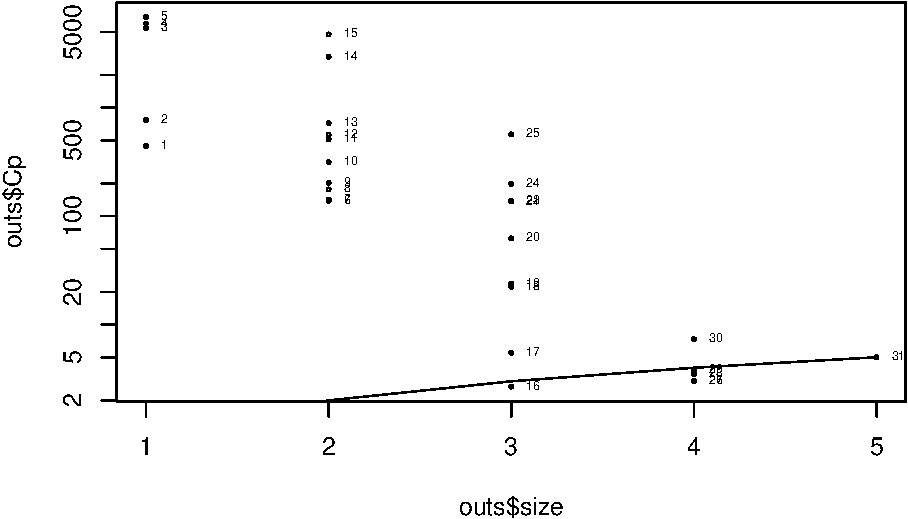
\includegraphics[keepaspectratio]{MultivariateStatisticalAnalysis_files/figure-latex/unnamed-chunk-75-1.pdf}}

\begin{Shaded}
\begin{Highlighting}[]
\CommentTok{\#Mejor modelo por la regla Cp ≈ p  (p = número de predictores)}

\NormalTok{idx\_best\_rule }\OtherTok{\textless{}{-}} \FunctionTok{which.min}\NormalTok{(}\FunctionTok{abs}\NormalTok{(outs}\SpecialCharTok{$}\NormalTok{Cp }\SpecialCharTok{{-}}\NormalTok{ outs}\SpecialCharTok{$}\NormalTok{size))}

\CommentTok{\#Variables que entran en cada mejor modelo}
\NormalTok{noms\_x }\OtherTok{\textless{}{-}} \FunctionTok{colnames}\NormalTok{(modelo.full}\SpecialCharTok{$}\NormalTok{x)            }\CommentTok{\# nombres de los predictores}
\NormalTok{vars\_rule  }\OtherTok{\textless{}{-}}\NormalTok{ noms\_x[ outs}\SpecialCharTok{$}\NormalTok{which[idx\_best\_rule, ] ]}

\NormalTok{vars\_rule}
\end{Highlighting}
\end{Shaded}

\begin{verbatim}
## [1] "(Intercept)" "x1"          "x2"          "x3"          "x4"
\end{verbatim}

Recordemos que nos interesan los modelos en los que \(C_p=p\).

\textbf{Ejemplo 2:} Vamos a usar la base de datos \texttt{mtcars}. Otra manera de analizar todos los modelos posibles:

\begin{Shaded}
\begin{Highlighting}[]
\FunctionTok{library}\NormalTok{(olsrr)}
\NormalTok{modelo.full.cars}\OtherTok{\textless{}{-}}\FunctionTok{lm}\NormalTok{(mpg}\SpecialCharTok{\textasciitilde{}}\NormalTok{., mtcars)}
\NormalTok{ejemplo}\OtherTok{\textless{}{-}}\FunctionTok{ols\_step\_all\_possible}\NormalTok{(modelo.full.cars)}
\FunctionTok{plot}\NormalTok{(ejemplo)}
\end{Highlighting}
\end{Shaded}

\pandocbounded{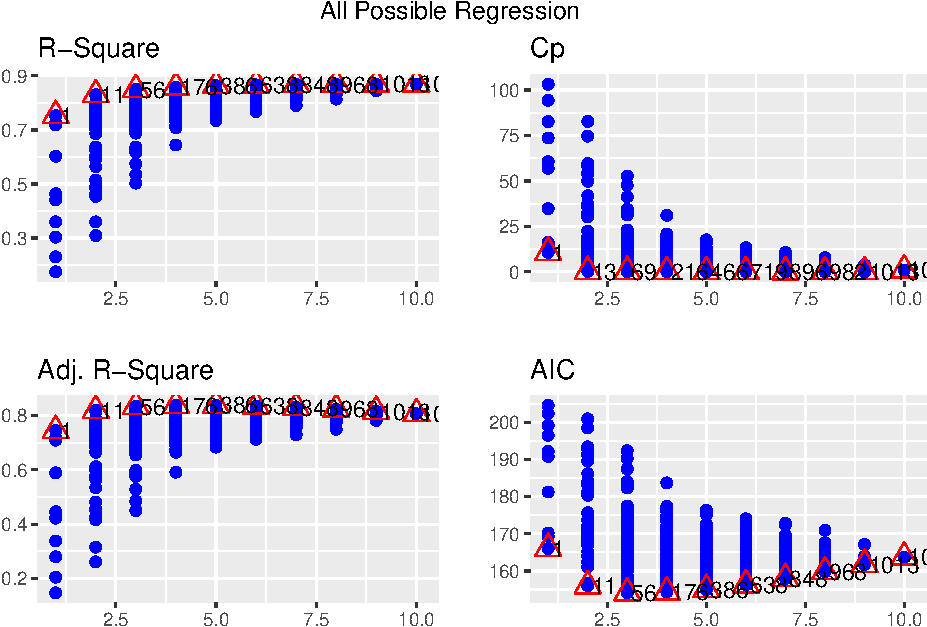
\includegraphics[keepaspectratio]{MultivariateStatisticalAnalysis_files/figure-latex/unnamed-chunk-77-1.pdf}} \pandocbounded{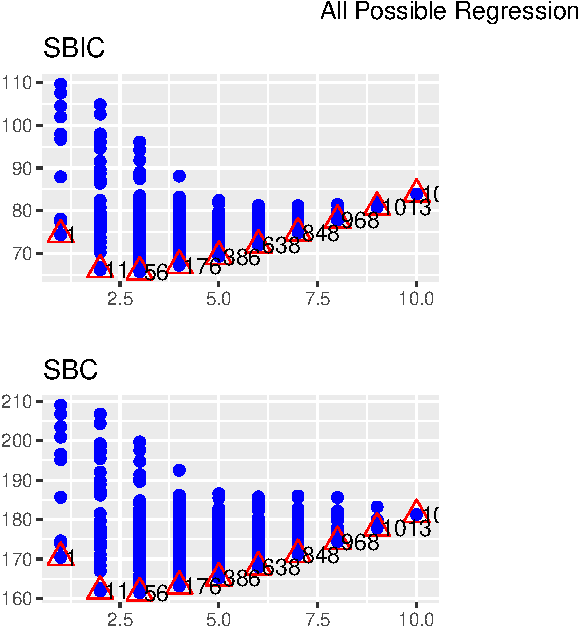
\includegraphics[keepaspectratio]{MultivariateStatisticalAnalysis_files/figure-latex/unnamed-chunk-77-2.pdf}}

Observe que en los triángulos rojos aparecen los mejores modelos para cada \(p\) en función de la estadística correspondiente.

\textbf{Ejemplo 3:} R tiene una función que nos muestra el mejor modelo para cada número de variables. Vamos a regresar al conjunto de datos \texttt{cemento}.

\begin{Shaded}
\begin{Highlighting}[]
\NormalTok{mejor}\OtherTok{\textless{}{-}}\FunctionTok{regsubsets}\NormalTok{(y}\SpecialCharTok{\textasciitilde{}}\NormalTok{., cemento)}
\FunctionTok{summary}\NormalTok{(mejor)}
\end{Highlighting}
\end{Shaded}

\begin{verbatim}
## Subset selection object
## Call: regsubsets.formula(y ~ ., cemento)
## 4 Variables  (and intercept)
##    Forced in Forced out
## x1     FALSE      FALSE
## x2     FALSE      FALSE
## x3     FALSE      FALSE
## x4     FALSE      FALSE
## 1 subsets of each size up to 4
## Selection Algorithm: exhaustive
##          x1  x2  x3  x4 
## 1  ( 1 ) " " " " " " "*"
## 2  ( 1 ) "*" "*" " " " "
## 3  ( 1 ) "*" "*" " " "*"
## 4  ( 1 ) "*" "*" "*" "*"
\end{verbatim}

\begin{Shaded}
\begin{Highlighting}[]
\FunctionTok{plot}\NormalTok{(mejor,}\AttributeTok{scale=}\StringTok{"Cp"}\NormalTok{) }
\end{Highlighting}
\end{Shaded}

\pandocbounded{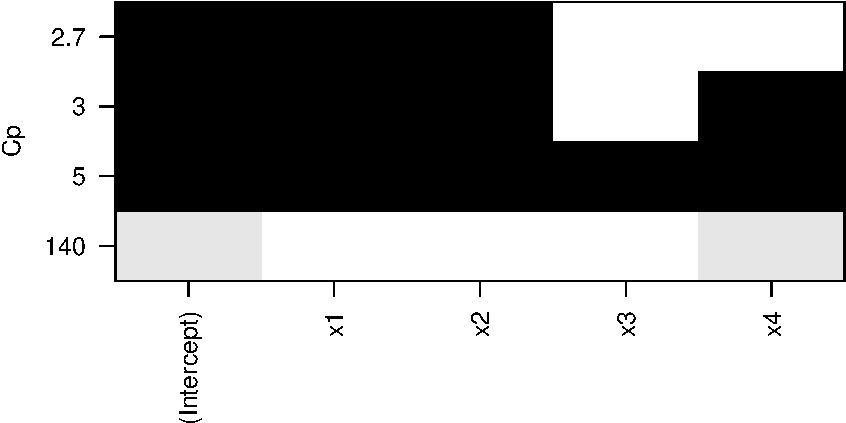
\includegraphics[keepaspectratio]{MultivariateStatisticalAnalysis_files/figure-latex/unnamed-chunk-78-1.pdf}}

La gráfica muestra los cuatro modelos y su \(C_p\), por ejemplo, el modelo que incluye al intercepto, a \(x_1\) y a \(x_2\) tiene una \(C_p\) cercana a 2.7.

\subsection{Selección paso a paso}\label{selecciuxf3n-paso-a-paso-1}

\textbf{Ejemplo 1:} Para analizar el método de selección paso a paso usaremos los datos \emph{swiss} del paquete \emph{MASS}. Para ello, el primer paso es ajustar el modelo con TODAS las variables independientes

\begin{Shaded}
\begin{Highlighting}[]
\FunctionTok{library}\NormalTok{(MASS)}
\end{Highlighting}
\end{Shaded}

\begin{verbatim}
## 
## Adjuntando el paquete: 'MASS'
\end{verbatim}

\begin{verbatim}
## The following object is masked from 'package:olsrr':
## 
##     cement
\end{verbatim}

\begin{verbatim}
## The following object is masked from 'package:patchwork':
## 
##     area
\end{verbatim}

\begin{verbatim}
## The following object is masked from 'package:dplyr':
## 
##     select
\end{verbatim}

\begin{Shaded}
\begin{Highlighting}[]
\NormalTok{modelo\_completo}\OtherTok{\textless{}{-}}\FunctionTok{lm}\NormalTok{(Fertility}\SpecialCharTok{\textasciitilde{}}\NormalTok{., swiss)}
\end{Highlighting}
\end{Shaded}

Podemos usar la función \emph{step} en las tres direcciones (\emph{forward, backward o both})

\begin{Shaded}
\begin{Highlighting}[]
\NormalTok{paso\_a\_paso}\OtherTok{\textless{}{-}}\FunctionTok{stepAIC}\NormalTok{(modelo\_completo, }\AttributeTok{direction=}\StringTok{"both"}\NormalTok{, }\AttributeTok{trace=}\NormalTok{T)}
\end{Highlighting}
\end{Shaded}

\begin{verbatim}
## Start:  AIC=190.69
## Fertility ~ Agriculture + Examination + Education + Catholic + 
##     Infant.Mortality
## 
##                    Df Sum of Sq    RSS    AIC
## - Examination       1     53.03 2158.1 189.86
## <none>                          2105.0 190.69
## - Agriculture       1    307.72 2412.8 195.10
## - Infant.Mortality  1    408.75 2513.8 197.03
## - Catholic          1    447.71 2552.8 197.75
## - Education         1   1162.56 3267.6 209.36
## 
## Step:  AIC=189.86
## Fertility ~ Agriculture + Education + Catholic + Infant.Mortality
## 
##                    Df Sum of Sq    RSS    AIC
## <none>                          2158.1 189.86
## + Examination       1     53.03 2105.0 190.69
## - Agriculture       1    264.18 2422.2 193.29
## - Infant.Mortality  1    409.81 2567.9 196.03
## - Catholic          1    956.57 3114.6 205.10
## - Education         1   2249.97 4408.0 221.43
\end{verbatim}

\begin{Shaded}
\begin{Highlighting}[]
\FunctionTok{summary}\NormalTok{(paso\_a\_paso)}
\end{Highlighting}
\end{Shaded}

\begin{verbatim}
## 
## Call:
## lm(formula = Fertility ~ Agriculture + Education + Catholic + 
##     Infant.Mortality, data = swiss)
## 
## Residuals:
##      Min       1Q   Median       3Q      Max 
## -14.6765  -6.0522   0.7514   3.1664  16.1422 
## 
## Coefficients:
##                  Estimate Std. Error t value Pr(>|t|)    
## (Intercept)      62.10131    9.60489   6.466 8.49e-08 ***
## Agriculture      -0.15462    0.06819  -2.267  0.02857 *  
## Education        -0.98026    0.14814  -6.617 5.14e-08 ***
## Catholic          0.12467    0.02889   4.315 9.50e-05 ***
## Infant.Mortality  1.07844    0.38187   2.824  0.00722 ** 
## ---
## Signif. codes:  0 '***' 0.001 '**' 0.01 '*' 0.05 '.' 0.1 ' ' 1
## 
## Residual standard error: 7.168 on 42 degrees of freedom
## Multiple R-squared:  0.6993, Adjusted R-squared:  0.6707 
## F-statistic: 24.42 on 4 and 42 DF,  p-value: 1.717e-10
\end{verbatim}

\textbf{Ejemplo 2:} O podemos usar el paquete \emph{olsrr}. Base de datos \texttt{surgical}.

\begin{Shaded}
\begin{Highlighting}[]
\NormalTok{modelo\_completo\_sur}\OtherTok{\textless{}{-}}\FunctionTok{lm}\NormalTok{(y}\SpecialCharTok{\textasciitilde{}}\NormalTok{., surgical)}
\FunctionTok{ols\_step\_forward\_aic}\NormalTok{(modelo\_completo\_sur, }\AttributeTok{details =}\NormalTok{ T)}
\end{Highlighting}
\end{Shaded}

\begin{verbatim}
## Forward Selection Method 
## ------------------------
## 
## Candidate Terms: 
## 
## 1. bcs 
## 2. pindex 
## 3. enzyme_test 
## 4. liver_test 
## 5. age 
## 6. gender 
## 7. alc_mod 
## 8. alc_heavy 
## 
## 
## Step     => 0 
## Model    => y ~ 1 
## AIC      => 802.606 
## 
## Initiating stepwise selection... 
## 
##                        Table: Adding New Variables                        
## -------------------------------------------------------------------------
## Predictor      DF      AIC        SBC       SBIC        R2       Adj. R2  
## -------------------------------------------------------------------------
## liver_test      1    771.875    777.842    616.009    0.45454     0.44405 
## enzyme_test     1    782.629    788.596    626.220    0.33435     0.32154 
## pindex          1    794.100    800.067    637.196    0.17680     0.16097 
## alc_heavy       1    794.301    800.268    637.389    0.17373     0.15784 
## bcs             1    797.697    803.664    640.655    0.12010     0.10318 
## alc_mod         1    802.828    808.795    645.601    0.03239     0.01378 
## gender          1    802.956    808.923    645.725    0.03009     0.01143 
## age             1    803.834    809.801    646.572    0.01420    -0.00476 
## -------------------------------------------------------------------------
## 
## Step     => 1 
## Added    => liver_test 
## Model    => y ~ liver_test 
## AIC      => 771.8753 
## 
##                       Table: Adding New Variables                        
## ------------------------------------------------------------------------
## Predictor      DF      AIC        SBC       SBIC        R2       Adj. R2 
## ------------------------------------------------------------------------
## alc_heavy       1    761.439    769.395    605.506    0.56674    0.54975 
## enzyme_test     1    762.077    770.033    606.090    0.56159    0.54440 
## pindex          1    770.387    778.343    613.737    0.48866    0.46861 
## alc_mod         1    771.141    779.097    614.435    0.48147    0.46113 
## gender          1    773.802    781.758    616.901    0.45528    0.43391 
## age             1    773.831    781.787    616.928    0.45498    0.43361 
## bcs             1    773.867    781.823    616.961    0.45462    0.43323 
## ------------------------------------------------------------------------
## 
## Step     => 2 
## Added    => alc_heavy 
## Model    => y ~ liver_test + alc_heavy 
## AIC      => 761.4394 
## 
##                       Table: Adding New Variables                        
## ------------------------------------------------------------------------
## Predictor      DF      AIC        SBC       SBIC        R2       Adj. R2 
## ------------------------------------------------------------------------
## enzyme_test     1    750.509    760.454    595.297    0.65900    0.63854 
## pindex          1    756.125    766.070    600.225    0.62163    0.59892 
## bcs             1    763.063    773.008    606.379    0.56975    0.54394 
## age             1    763.110    773.055    606.421    0.56938    0.54354 
## alc_mod         1    763.428    773.373    606.704    0.56683    0.54084 
## gender          1    763.433    773.378    606.709    0.56679    0.54080 
## ------------------------------------------------------------------------
## 
## Step     => 3 
## Added    => enzyme_test 
## Model    => y ~ liver_test + alc_heavy + enzyme_test 
## AIC      => 750.5089 
## 
##                      Table: Adding New Variables                       
## ----------------------------------------------------------------------
## Predictor    DF      AIC        SBC       SBIC        R2       Adj. R2 
## ----------------------------------------------------------------------
## pindex        1    735.715    747.649    582.943    0.75015    0.72975 
## bcs           1    750.782    762.716    595.377    0.66973    0.64277 
## alc_mod       1    752.403    764.337    596.743    0.65967    0.63189 
## age           1    752.416    764.350    596.755    0.65959    0.63180 
## gender        1    752.509    764.443    596.833    0.65900    0.63116 
## ----------------------------------------------------------------------
## 
## Step     => 4 
## Added    => pindex 
## Model    => y ~ liver_test + alc_heavy + enzyme_test + pindex 
## AIC      => 735.7146 
## 
##                      Table: Adding New Variables                       
## ----------------------------------------------------------------------
## Predictor    DF      AIC        SBC       SBIC        R2       Adj. R2 
## ----------------------------------------------------------------------
## bcs           1    730.620    744.543    579.638    0.78091    0.75808 
## age           1    737.680    751.603    585.012    0.75030    0.72429 
## gender        1    737.712    751.635    585.036    0.75016    0.72413 
## alc_mod       1    737.713    751.636    585.037    0.75015    0.72413 
## ----------------------------------------------------------------------
## 
## Step     => 5 
## Added    => bcs 
## Model    => y ~ liver_test + alc_heavy + enzyme_test + pindex + bcs 
## AIC      => 730.6204 
## 
##                      Table: Adding New Variables                       
## ----------------------------------------------------------------------
## Predictor    DF      AIC        SBC       SBIC        R2       Adj. R2 
## ----------------------------------------------------------------------
## age           1    732.494    748.406    581.938    0.78142    0.75351 
## gender        1    732.551    748.463    581.978    0.78119    0.75325 
## alc_mod       1    732.614    748.526    582.023    0.78093    0.75297 
## ----------------------------------------------------------------------
## 
## 
## No more variables to be added.
## 
## Variables Selected: 
## 
## => liver_test 
## => alc_heavy 
## => enzyme_test 
## => pindex 
## => bcs
\end{verbatim}

\begin{verbatim}
## 
## 
##                               Stepwise Summary                              
## --------------------------------------------------------------------------
## Step    Variable         AIC        SBC       SBIC        R2       Adj. R2 
## --------------------------------------------------------------------------
##  0      Base Model     802.606    806.584    646.794    0.00000    0.00000 
##  1      liver_test     771.875    777.842    616.009    0.45454    0.44405 
##  2      alc_heavy      761.439    769.395    605.506    0.56674    0.54975 
##  3      enzyme_test    750.509    760.454    595.297    0.65900    0.63854 
##  4      pindex         735.715    747.649    582.943    0.75015    0.72975 
##  5      bcs            730.620    744.543    579.638    0.78091    0.75808 
## --------------------------------------------------------------------------
## 
## Final Model Output 
## ------------------
## 
##                            Model Summary                            
## -------------------------------------------------------------------
## R                         0.884       RMSE                 184.276 
## R-Squared                 0.781       MSE                33957.712 
## Adj. R-Squared            0.758       Coef. Var             27.839 
## Pred R-Squared            0.700       AIC                  730.620 
## MAE                     137.656       SBC                  744.543 
## -------------------------------------------------------------------
##  RMSE: Root Mean Square Error 
##  MSE: Mean Square Error 
##  MAE: Mean Absolute Error 
##  AIC: Akaike Information Criteria 
##  SBC: Schwarz Bayesian Criteria 
## 
##                                  ANOVA                                  
## -----------------------------------------------------------------------
##                    Sum of                                              
##                   Squares        DF    Mean Square      F         Sig. 
## -----------------------------------------------------------------------
## Regression    6535804.090         5    1307160.818    34.217    0.0000 
## Residual      1833716.447        48      38202.426                     
## Total         8369520.537        53                                    
## -----------------------------------------------------------------------
## 
##                                       Parameter Estimates                                        
## ------------------------------------------------------------------------------------------------
##       model         Beta    Std. Error    Std. Beta      t        Sig         lower       upper 
## ------------------------------------------------------------------------------------------------
## (Intercept)    -1178.330       208.682                 -5.647    0.000    -1597.914    -758.746 
##  liver_test       58.064        40.144        0.156     1.446    0.155      -22.652     138.779 
##   alc_heavy      317.848        71.634        0.314     4.437    0.000      173.818     461.878 
## enzyme_test        9.748         1.656        0.521     5.887    0.000        6.419      13.077 
##      pindex        8.924         1.808        0.380     4.935    0.000        5.288      12.559 
##         bcs       59.864        23.060        0.241     2.596    0.012       13.498     106.230 
## ------------------------------------------------------------------------------------------------
\end{verbatim}

\begin{Shaded}
\begin{Highlighting}[]
\FunctionTok{ols\_step\_backward\_aic}\NormalTok{(modelo\_completo\_sur)}
\end{Highlighting}
\end{Shaded}

\begin{verbatim}
## 
## 
##                              Stepwise Summary                              
## -------------------------------------------------------------------------
## Step    Variable        AIC        SBC       SBIC        R2       Adj. R2 
## -------------------------------------------------------------------------
##  0      Full Model    736.390    756.280    586.665    0.78184    0.74305 
##  1      alc_mod       734.407    752.308    583.884    0.78177    0.74856 
##  2      gender        732.494    748.406    581.290    0.78142    0.75351 
##  3      age           730.620    744.543    578.844    0.78091    0.75808 
## -------------------------------------------------------------------------
## 
## Final Model Output 
## ------------------
## 
##                            Model Summary                            
## -------------------------------------------------------------------
## R                         0.884       RMSE                 184.276 
## R-Squared                 0.781       MSE                33957.712 
## Adj. R-Squared            0.758       Coef. Var             27.839 
## Pred R-Squared            0.700       AIC                  730.620 
## MAE                     137.656       SBC                  744.543 
## -------------------------------------------------------------------
##  RMSE: Root Mean Square Error 
##  MSE: Mean Square Error 
##  MAE: Mean Absolute Error 
##  AIC: Akaike Information Criteria 
##  SBC: Schwarz Bayesian Criteria 
## 
##                                  ANOVA                                  
## -----------------------------------------------------------------------
##                    Sum of                                              
##                   Squares        DF    Mean Square      F         Sig. 
## -----------------------------------------------------------------------
## Regression    6535804.090         5    1307160.818    34.217    0.0000 
## Residual      1833716.447        48      38202.426                     
## Total         8369520.537        53                                    
## -----------------------------------------------------------------------
## 
##                                       Parameter Estimates                                        
## ------------------------------------------------------------------------------------------------
##       model         Beta    Std. Error    Std. Beta      t        Sig         lower       upper 
## ------------------------------------------------------------------------------------------------
## (Intercept)    -1178.330       208.682                 -5.647    0.000    -1597.914    -758.746 
##         bcs       59.864        23.060        0.241     2.596    0.012       13.498     106.230 
##      pindex        8.924         1.808        0.380     4.935    0.000        5.288      12.559 
## enzyme_test        9.748         1.656        0.521     5.887    0.000        6.419      13.077 
##  liver_test       58.064        40.144        0.156     1.446    0.155      -22.652     138.779 
##   alc_heavy      317.848        71.634        0.314     4.437    0.000      173.818     461.878 
## ------------------------------------------------------------------------------------------------
\end{verbatim}

\begin{Shaded}
\begin{Highlighting}[]
\FunctionTok{ols\_step\_forward\_aic}\NormalTok{(modelo\_completo\_sur)}
\end{Highlighting}
\end{Shaded}

\begin{verbatim}
## 
## 
##                               Stepwise Summary                              
## --------------------------------------------------------------------------
## Step    Variable         AIC        SBC       SBIC        R2       Adj. R2 
## --------------------------------------------------------------------------
##  0      Base Model     802.606    806.584    646.794    0.00000    0.00000 
##  1      liver_test     771.875    777.842    616.009    0.45454    0.44405 
##  2      alc_heavy      761.439    769.395    605.506    0.56674    0.54975 
##  3      enzyme_test    750.509    760.454    595.297    0.65900    0.63854 
##  4      pindex         735.715    747.649    582.943    0.75015    0.72975 
##  5      bcs            730.620    744.543    579.638    0.78091    0.75808 
## --------------------------------------------------------------------------
## 
## Final Model Output 
## ------------------
## 
##                            Model Summary                            
## -------------------------------------------------------------------
## R                         0.884       RMSE                 184.276 
## R-Squared                 0.781       MSE                33957.712 
## Adj. R-Squared            0.758       Coef. Var             27.839 
## Pred R-Squared            0.700       AIC                  730.620 
## MAE                     137.656       SBC                  744.543 
## -------------------------------------------------------------------
##  RMSE: Root Mean Square Error 
##  MSE: Mean Square Error 
##  MAE: Mean Absolute Error 
##  AIC: Akaike Information Criteria 
##  SBC: Schwarz Bayesian Criteria 
## 
##                                  ANOVA                                  
## -----------------------------------------------------------------------
##                    Sum of                                              
##                   Squares        DF    Mean Square      F         Sig. 
## -----------------------------------------------------------------------
## Regression    6535804.090         5    1307160.818    34.217    0.0000 
## Residual      1833716.447        48      38202.426                     
## Total         8369520.537        53                                    
## -----------------------------------------------------------------------
## 
##                                       Parameter Estimates                                        
## ------------------------------------------------------------------------------------------------
##       model         Beta    Std. Error    Std. Beta      t        Sig         lower       upper 
## ------------------------------------------------------------------------------------------------
## (Intercept)    -1178.330       208.682                 -5.647    0.000    -1597.914    -758.746 
##  liver_test       58.064        40.144        0.156     1.446    0.155      -22.652     138.779 
##   alc_heavy      317.848        71.634        0.314     4.437    0.000      173.818     461.878 
## enzyme_test        9.748         1.656        0.521     5.887    0.000        6.419      13.077 
##      pindex        8.924         1.808        0.380     4.935    0.000        5.288      12.559 
##         bcs       59.864        23.060        0.241     2.596    0.012       13.498     106.230 
## ------------------------------------------------------------------------------------------------
\end{verbatim}

Ojo: el parámetro \emph{details=T} nos dará en detalle el proceso con el que se llegó al modelo correspondiente. También hay que tener en cuenta que podríamos llegar a modelos diferentes si usamos métodos diferentes.

Si podemos llegar a resultados diferentes, ¿cómo sabemos cuál es el mejor modelo?.

Recordemos que estos métodos se basan en UNA SOLA estadística para ir mejorando el modelo, de manera que, aunque tengamos el modelo con el AIC menor, este podría no ser el mejor en términos del cumplimiento de los supuestos.

\textbf{Ejemplo 3} Veamos con mas detalle el modelo de \emph{cement.txt}.

\begin{Shaded}
\begin{Highlighting}[]
\CommentTok{\#Modelo elegido por el algoritmo}
\NormalTok{modelo.bueno}\OtherTok{\textless{}{-}}\FunctionTok{lm}\NormalTok{(y}\SpecialCharTok{\textasciitilde{}}\NormalTok{.}\SpecialCharTok{{-}}\NormalTok{x3, cemento)}
\FunctionTok{summary}\NormalTok{(modelo.bueno)}
\end{Highlighting}
\end{Shaded}

\begin{verbatim}
## 
## Call:
## lm(formula = y ~ . - x3, data = cemento)
## 
## Residuals:
##     Min      1Q  Median      3Q     Max 
## -3.0919 -1.8016  0.2562  1.2818  3.8982 
## 
## Coefficients:
##             Estimate Std. Error t value Pr(>|t|)    
## (Intercept)  71.6483    14.1424   5.066 0.000675 ***
## x1            1.4519     0.1170  12.410 5.78e-07 ***
## x2            0.4161     0.1856   2.242 0.051687 .  
## x4           -0.2365     0.1733  -1.365 0.205395    
## ---
## Signif. codes:  0 '***' 0.001 '**' 0.01 '*' 0.05 '.' 0.1 ' ' 1
## 
## Residual standard error: 2.309 on 9 degrees of freedom
## Multiple R-squared:  0.9823, Adjusted R-squared:  0.9764 
## F-statistic: 166.8 on 3 and 9 DF,  p-value: 3.323e-08
\end{verbatim}

\begin{Shaded}
\begin{Highlighting}[]
\CommentTok{\#Modelo sin x3 y x4}
\NormalTok{modelo}\FloatTok{.12}\OtherTok{\textless{}{-}}\FunctionTok{lm}\NormalTok{(y}\SpecialCharTok{\textasciitilde{}}\NormalTok{x1}\SpecialCharTok{+}\NormalTok{x2, cemento)}
\FunctionTok{summary}\NormalTok{(modelo}\FloatTok{.12}\NormalTok{)}
\end{Highlighting}
\end{Shaded}

\begin{verbatim}
## 
## Call:
## lm(formula = y ~ x1 + x2, data = cemento)
## 
## Residuals:
##    Min     1Q Median     3Q    Max 
## -2.893 -1.574 -1.302  1.363  4.048 
## 
## Coefficients:
##             Estimate Std. Error t value Pr(>|t|)    
## (Intercept) 52.57735    2.28617   23.00 5.46e-10 ***
## x1           1.46831    0.12130   12.11 2.69e-07 ***
## x2           0.66225    0.04585   14.44 5.03e-08 ***
## ---
## Signif. codes:  0 '***' 0.001 '**' 0.01 '*' 0.05 '.' 0.1 ' ' 1
## 
## Residual standard error: 2.406 on 10 degrees of freedom
## Multiple R-squared:  0.9787, Adjusted R-squared:  0.9744 
## F-statistic: 229.5 on 2 and 10 DF,  p-value: 4.407e-09
\end{verbatim}

\begin{Shaded}
\begin{Highlighting}[]
\CommentTok{\#Modelo sin x3 y x2}
\NormalTok{modelo}\FloatTok{.14}\OtherTok{\textless{}{-}}\FunctionTok{lm}\NormalTok{(y}\SpecialCharTok{\textasciitilde{}}\NormalTok{x1}\SpecialCharTok{+}\NormalTok{x4, cemento)}
\FunctionTok{summary}\NormalTok{(modelo}\FloatTok{.14}\NormalTok{)}
\end{Highlighting}
\end{Shaded}

\begin{verbatim}
## 
## Call:
## lm(formula = y ~ x1 + x4, data = cemento)
## 
## Residuals:
##     Min      1Q  Median      3Q     Max 
## -5.0234 -1.4737  0.1371  1.7305  3.7701 
## 
## Coefficients:
##              Estimate Std. Error t value Pr(>|t|)    
## (Intercept) 103.09738    2.12398   48.54 3.32e-13 ***
## x1            1.43996    0.13842   10.40 1.11e-06 ***
## x4           -0.61395    0.04864  -12.62 1.81e-07 ***
## ---
## Signif. codes:  0 '***' 0.001 '**' 0.01 '*' 0.05 '.' 0.1 ' ' 1
## 
## Residual standard error: 2.734 on 10 degrees of freedom
## Multiple R-squared:  0.9725, Adjusted R-squared:  0.967 
## F-statistic: 176.6 on 2 and 10 DF,  p-value: 1.581e-08
\end{verbatim}

Observamos que en el modelo que elige el algoritmo, la variable X4 no es significativa, y por el diagrama de disperisón vemos que está correlacionada con X2, por ello decidimos analizar el modelo eliminando X2 y X4. En ambos modelos las variables son significativas y \(R^2\) es alta.

Comparemos su AIC

\begin{Shaded}
\begin{Highlighting}[]
\FunctionTok{AIC}\NormalTok{(modelo.bueno, modelo}\FloatTok{.12}\NormalTok{, modelo}\FloatTok{.14}\NormalTok{)}
\end{Highlighting}
\end{Shaded}

\begin{verbatim}
##              df      AIC
## modelo.bueno  5 63.86629
## modelo.12     4 64.31239
## modelo.14     4 67.63411
\end{verbatim}

Entre los tres, preferimos al \emph{modelo.12} ya que es el segundo en \emph{R\^{}2}, todas las variables son significativas y, aunque no tiene el mínimo AIC, sí es muy parecido y es menor que el AIC del \emph{modelo.14}. Es decir, en conjunto es el \emph{modelo.12} es el que mejor cumple los supuestos y tiene buenas estadísticas.

\subsubsection{Ejercicios}\label{ejercicios-4}

\textbf{Ejercicio 1:} Para los datos de rendimiento de gasolina. Aplica los tres métodos vistos de selección de modelos. Compara los resultados y especifica cual sería el mejor modelo con cuales estadísticas.

\chapter{Análisis de Componentes Principales}\label{anuxe1lisis-de-componentes-principales}

\chapter{Análisis Factorial}\label{anuxe1lisis-factorial}

\chapter{Análisis de Conglomerados}\label{anuxe1lisis-de-conglomerados}

\chapter{Análisis de Discriminante}\label{anuxe1lisis-de-discriminante}

\chapter{Apéndices}\label{apuxe9ndices}

\section{Introducción a R}\label{introducciuxf3n-a-r}

\begin{itemize}
\item
  Tutorial de RMarkdown: \href{https://github.com/HaydeePeruyero/Rmarkdown_and_LaTeX/blob/main/ejemplo.Rmd}{Link}
\item
  Tutorial Manejo de Proyectos: \href{https://haydeeperuyero.github.io/Seminario_Estadistica/manejo-de-proyectos.html}{Link}
\end{itemize}

\section{Git + Github}\label{git-github}

\begin{itemize}
\tightlist
\item
  Conectar R con Git y Github: \href{https://r-ladies-morelia.github.io/blog/conectar/}{Link}
\end{itemize}

\section{Gráficas Multivariadas}\label{gruxe1ficas-multivariadas}

\section{Escalas de Medición}\label{escalas-de-mediciuxf3n}

\section{Valores Faltantes}\label{valores-faltantes}

  \bibliography{book.bib,packages.bib}

\end{document}
